
\section{3 lepton training for high $e_T^{miss}$ and invariant mass search}\label{sec:3lep}


To better accertain and map the usefulness of the regular and variational autoencoder in the search for 
new physics, two MC signals were used as test cases. They are both 3 lep +$e_T^{miss}$ final state SUSY signals,
and thus are a suitable fit to use for testing. The two autoencoders were tested on four metrics. 
\begin{itemize}
    \item Low reconstruction error on SM MC
    \item Background to signal ratio in $e_T^{miss}$ signal region
    \item Large tail or possible resonance in trilepton signal region
    \item Significance scan in $e_T^{miss}$ signal region
\end{itemize}



\subsubsection*{Regular autoencoder output}\label{sec:3lep_reg}


\begin{figure}[!htb]
    \centering
    \begin{subfigure}{.49\textwidth}
        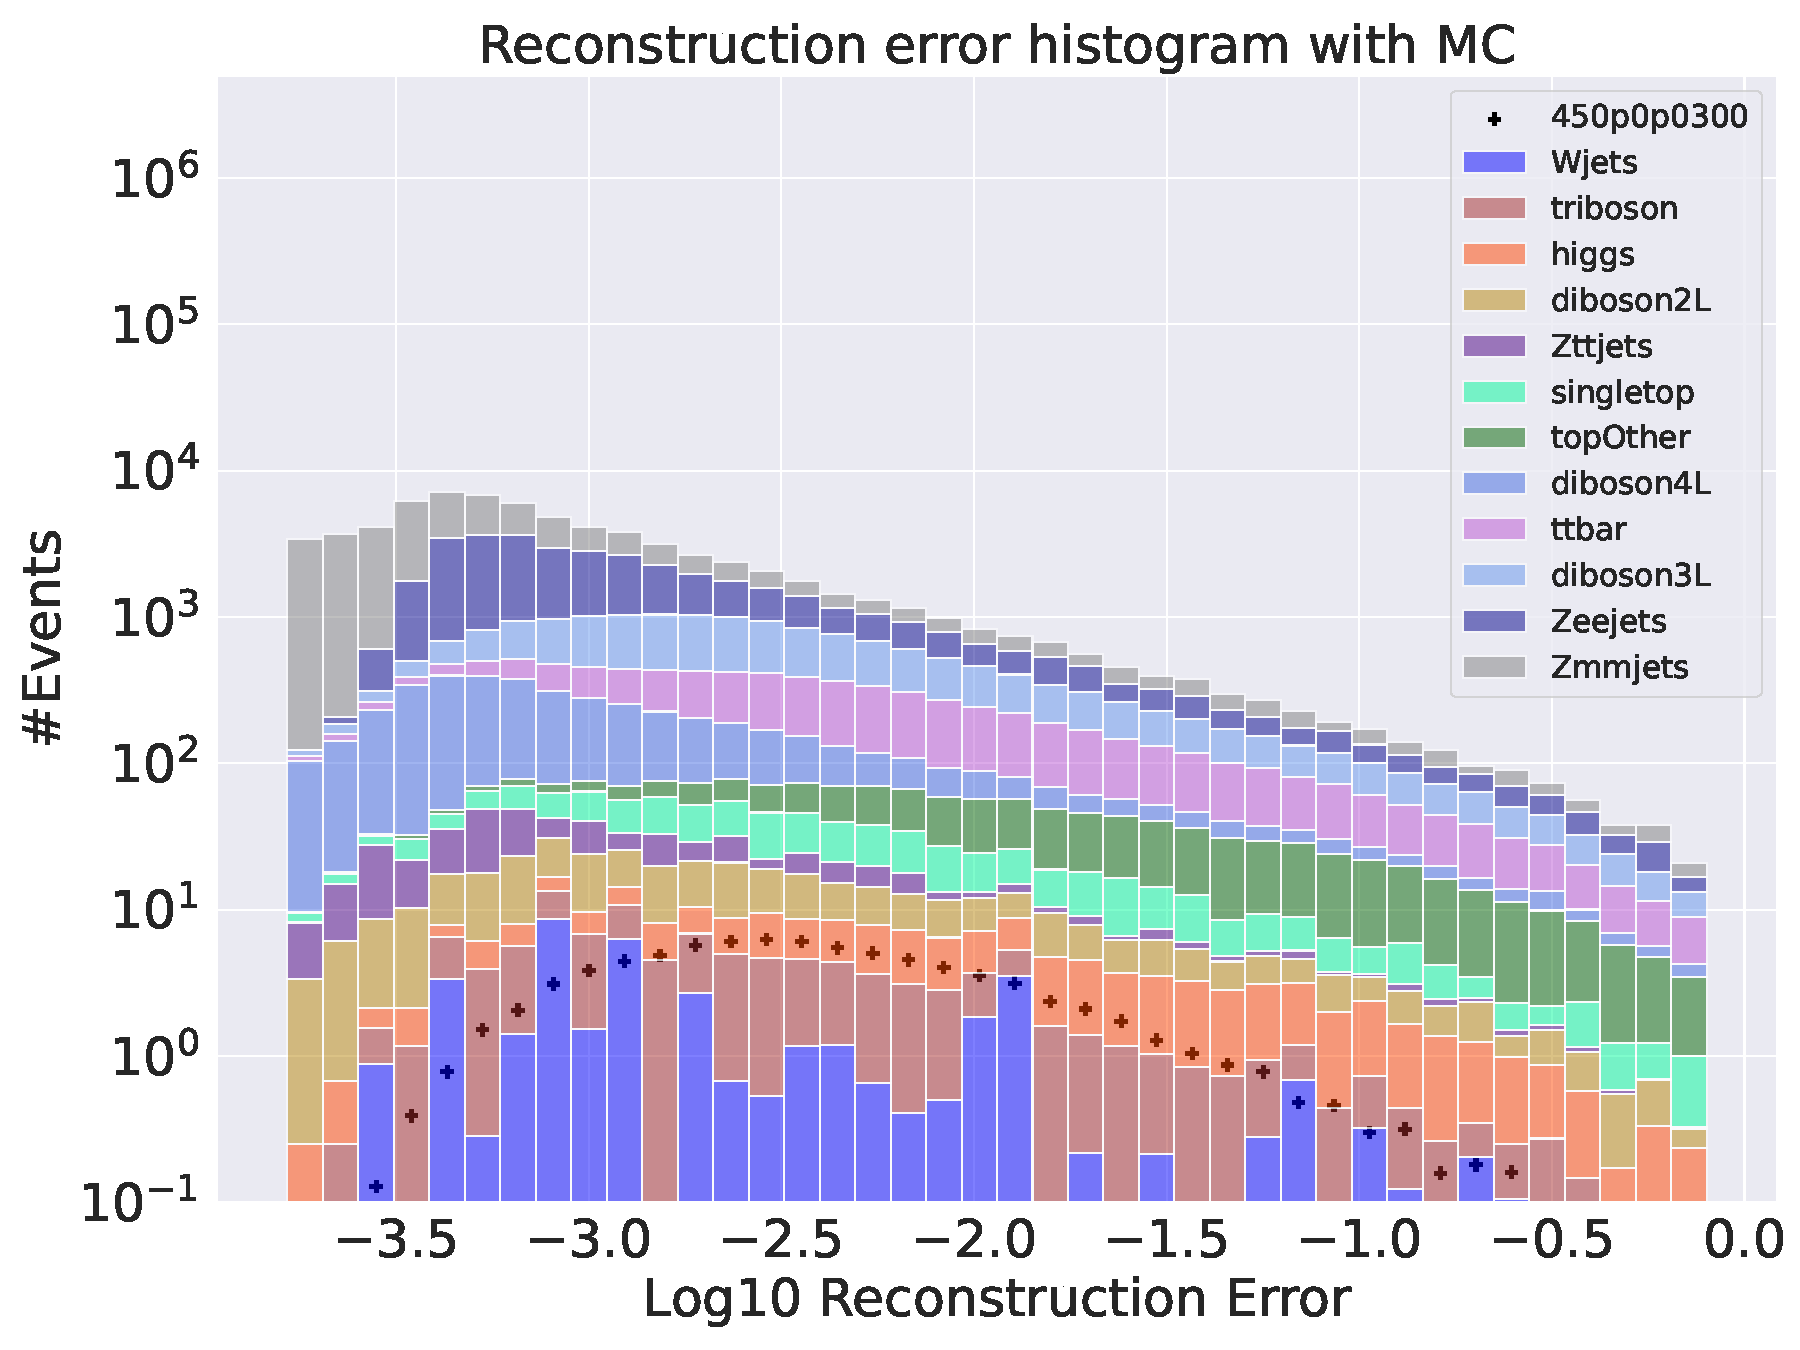
\includegraphics[width=\textwidth]{Figures/AE_testing/big/3lep/b_data_recon_big_rm3_feats_sig_450p0p0300.pdf}
        \caption{ }
        \label{fig:AE_3lep_big_450}
    \end{subfigure}
    \hfill
    \begin{subfigure}{.49\textwidth}
        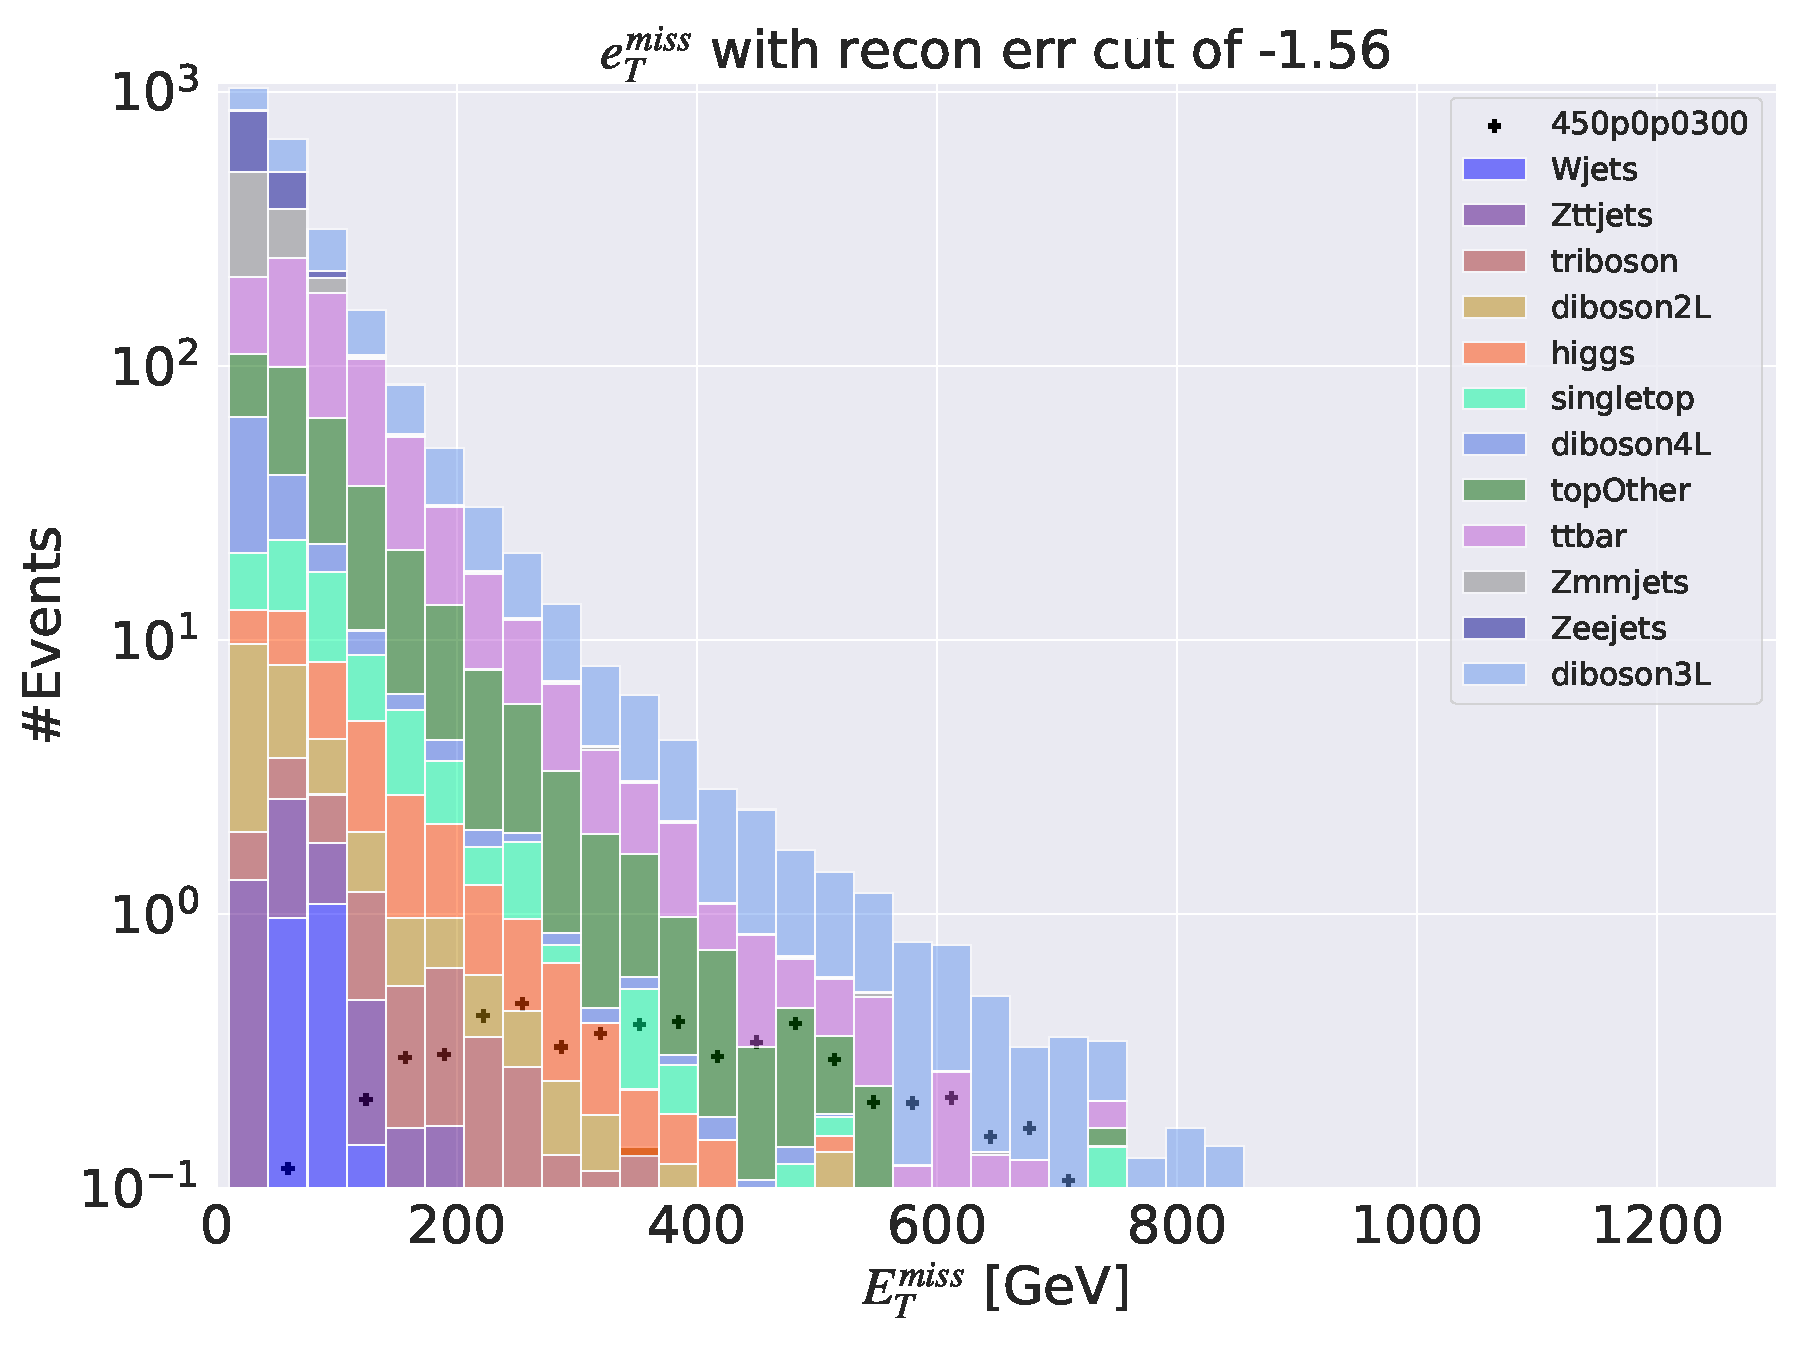
\includegraphics[width=\textwidth]{Figures/AE_testing/big/3lep/b_data_recon_big_rm3_feats_sig_450p0p0300_etmiss_recon_errcut_-1.56.pdf}
        \caption{}
        \label{fig:AE_3lep_big_etmiss_450}
    \end{subfigure}
    \hfill
    \begin{subfigure}{.49\textwidth}
        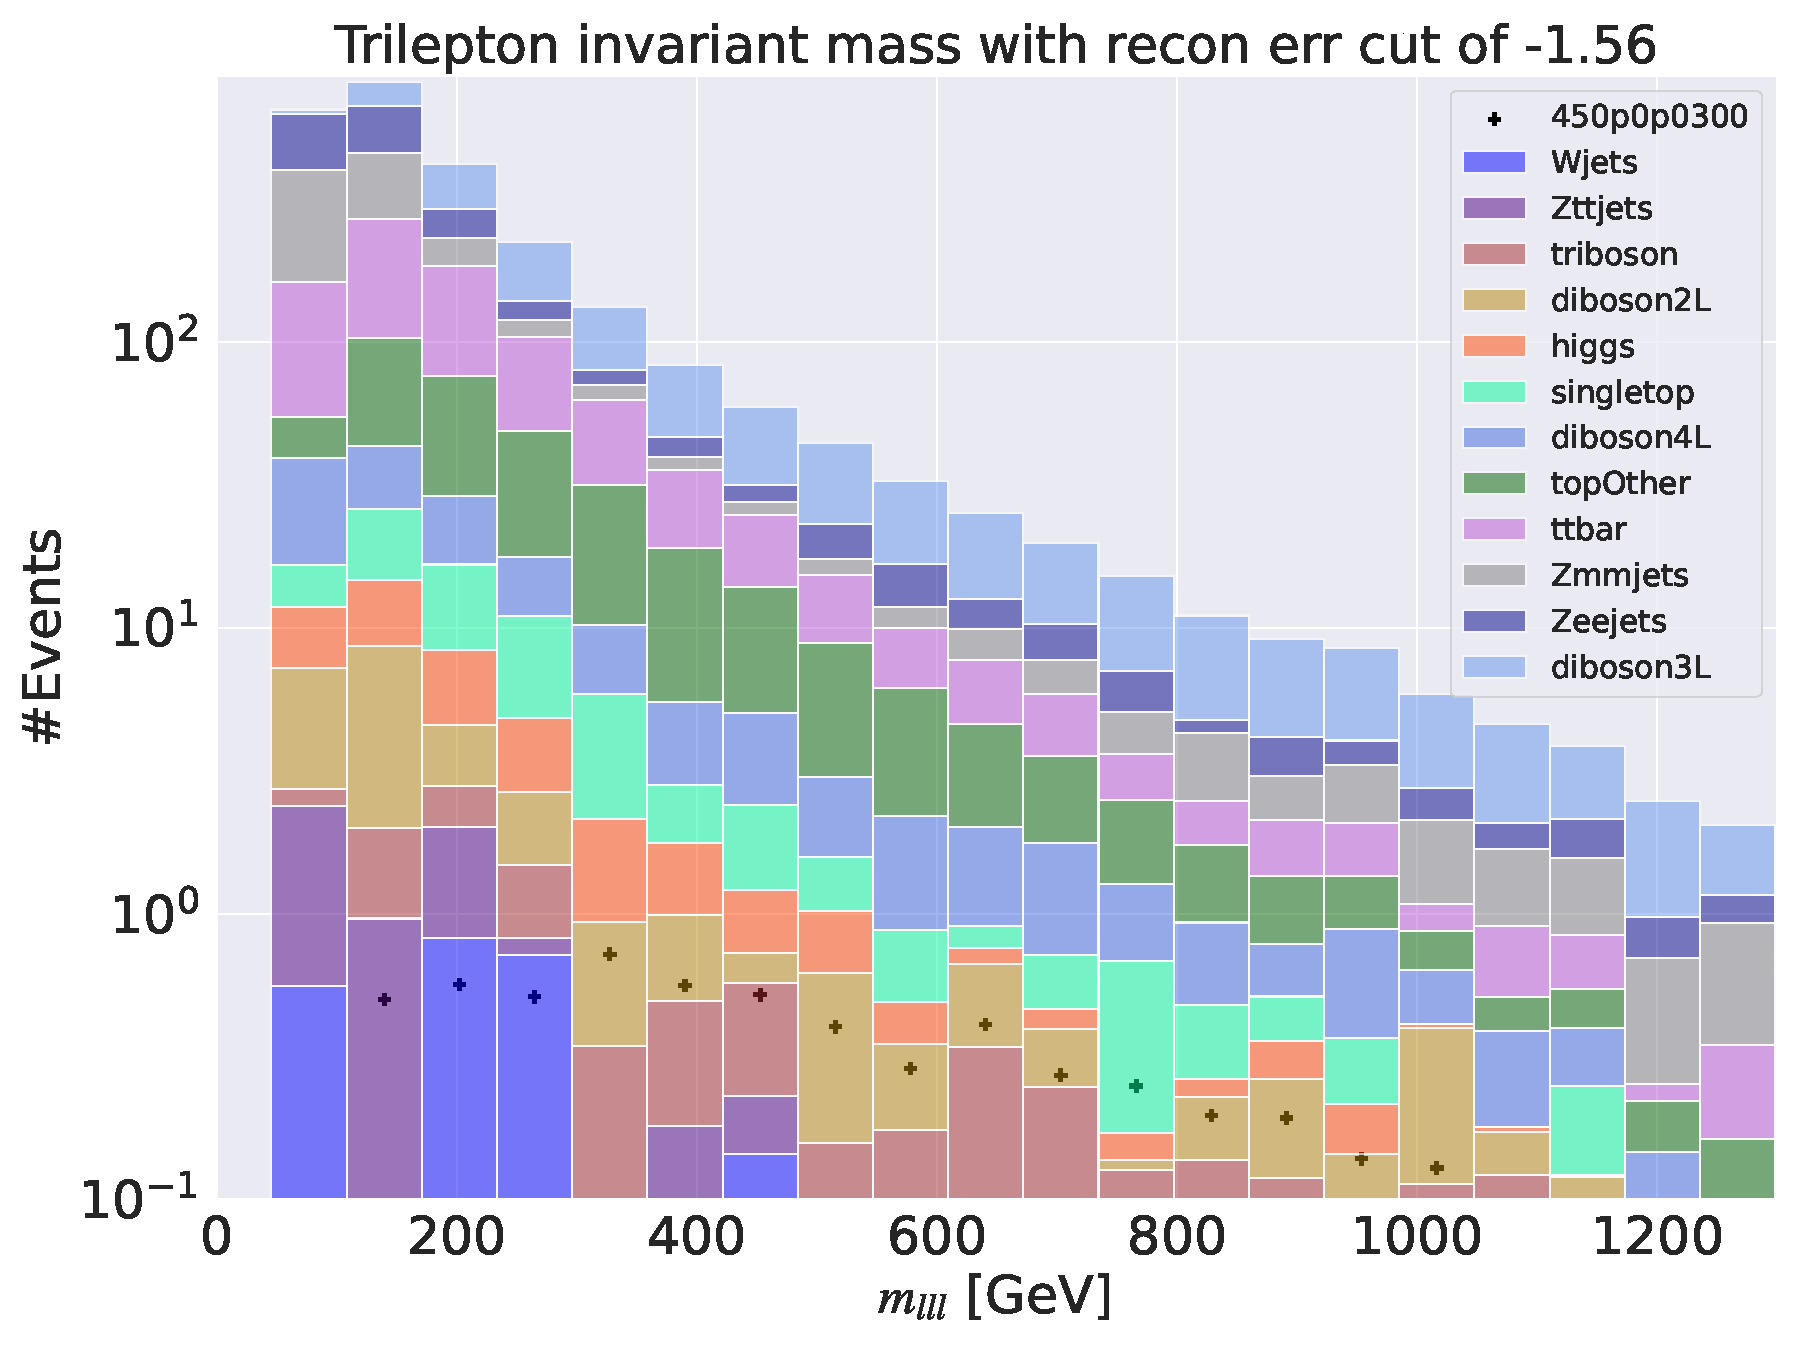
\includegraphics[width=\textwidth]{Figures/AE_testing/big/3lep/b_data_recon_big_rm3_feats_sig_450p0p0300_mlll_recon_errcut_-1.56.pdf}
        \caption{}
        \label{fig:AE_3lep_big_mlll_450}
    \end{subfigure}
    \hfill   
    \begin{subfigure}{.49\textwidth}
        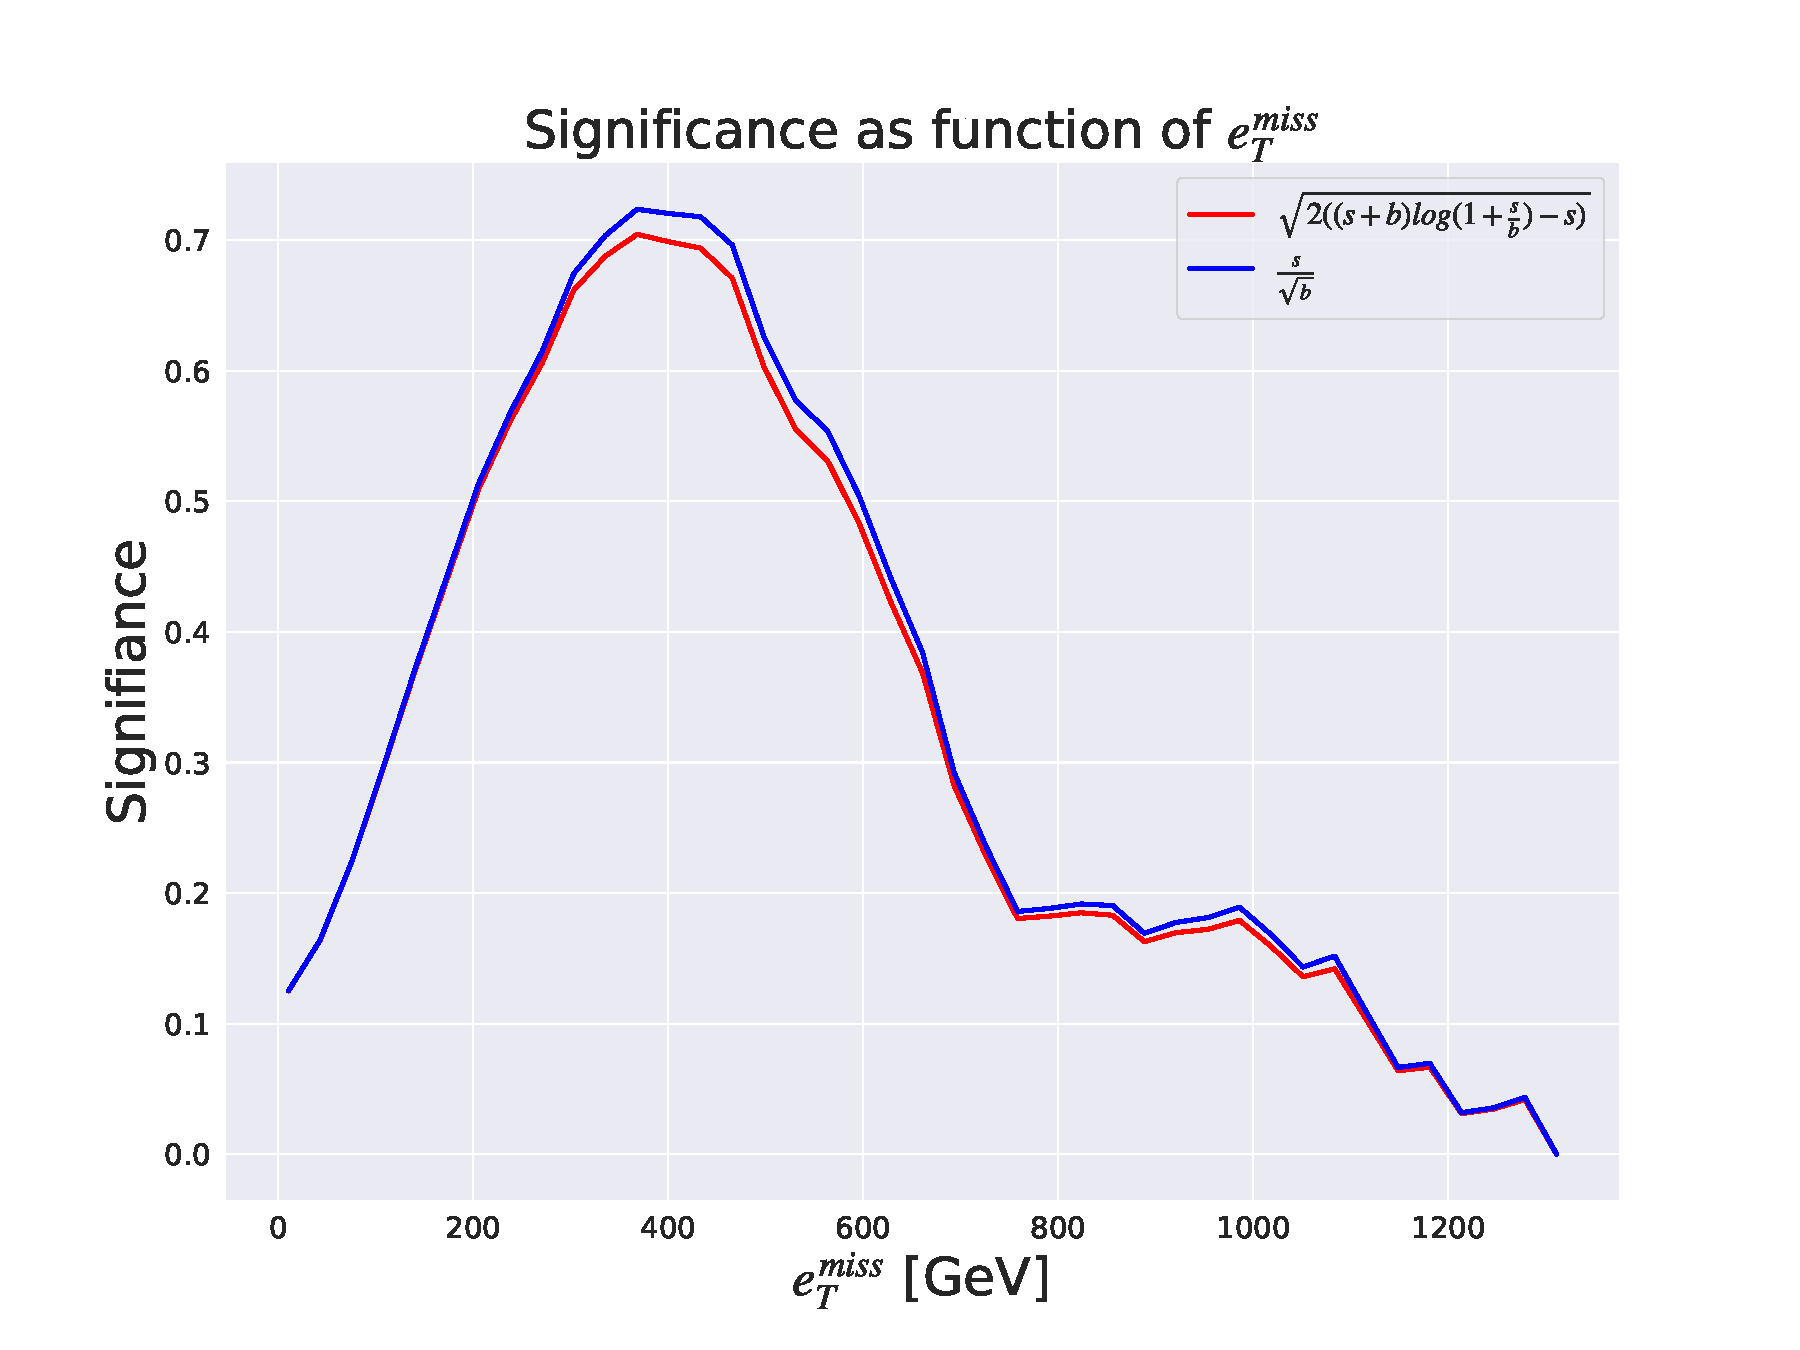
\includegraphics[width=\textwidth]{Figures/AE_testing/big/3lep/significance_etmiss_450p0p0300_-1.5648275418402864.pdf}
        \caption{}
        \label{fig:AE_3lep_big_signi_450}
    \end{subfigure}
    \hfill      
    \caption[3lep deep network | $450p300$ | AE]{Reconstruction error, $e_T^{miss}$ signal region, $m_{lll}$ signal region and significance as function of 
    $e_T^{miss}$ for the deep regular autoencoder using the SUSY $450p300$. 
    Figure \ref{fig:AE_3lep_big_450} shows the reconstruction error 
    distribution for the SM MC and the SUSY signal. Here the autoencoder produces the same reconstruction error shape for both background and 
    signal. Figure \ref{fig:AE_3lep_big_etmiss_450} shows the $e_T^{miss}$ distribution for the SM MC and the SUSY signal in the signal region, 
    defined as the region having a $log_{10}$ reconstruction error above -1.56. Most of the background is removed, and the signal 
    distribution is clearly shifted towards higher values of $e_T^{miss}$ compared with SM MC. Figure \ref{fig:AE_3lep_big_mlll_450} shows the $m_{lll}$ distribution for the SM MC and the SUSY signal. 
    The shape of the SM MC and the signal distributions are too similar to distinguish. Figure \ref{fig:AE_3lep_big_signi_450} shows the significance as function of
    $e_T^{miss}$. The maximum significance is found when applying a cut of about > 380 GeV in the $e_T^{miss}$, with a significance of around $0.7$. }
    \label{fig:AE_3lep_big_rec_sig_signi_450}
\end{figure}

\begin{figure}[!htb]
    \centering
    \begin{subfigure}{.49\textwidth}
        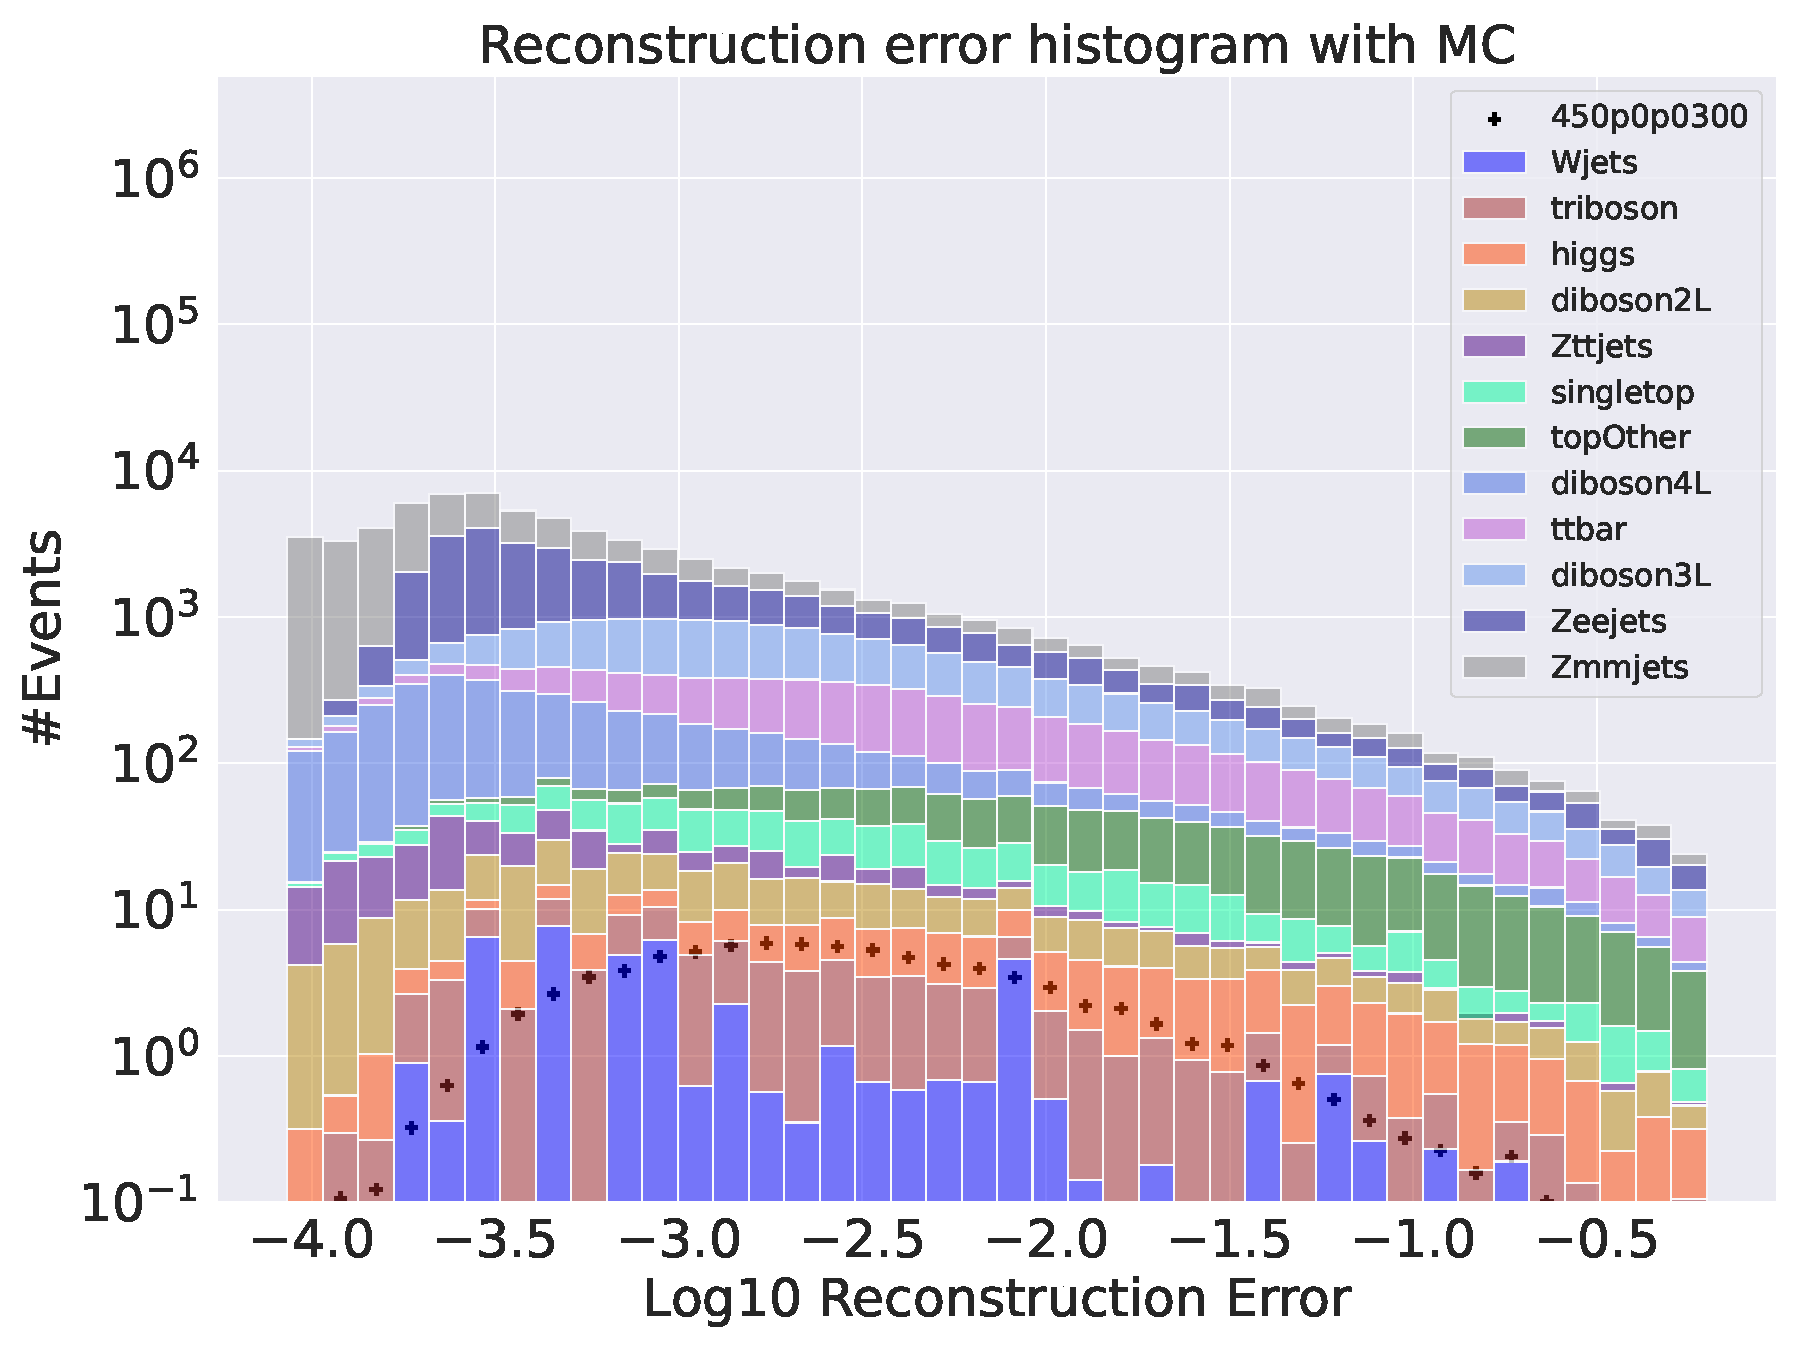
\includegraphics[width=\textwidth]{Figures/AE_testing/small/3lep/b_data_recon_big_rm3_feats_sig_450p0p0300.pdf}
        \caption{ }
        \label{fig:AE_3lep_small_450}
    \end{subfigure}
    \hfill
    \begin{subfigure}{.49\textwidth}
        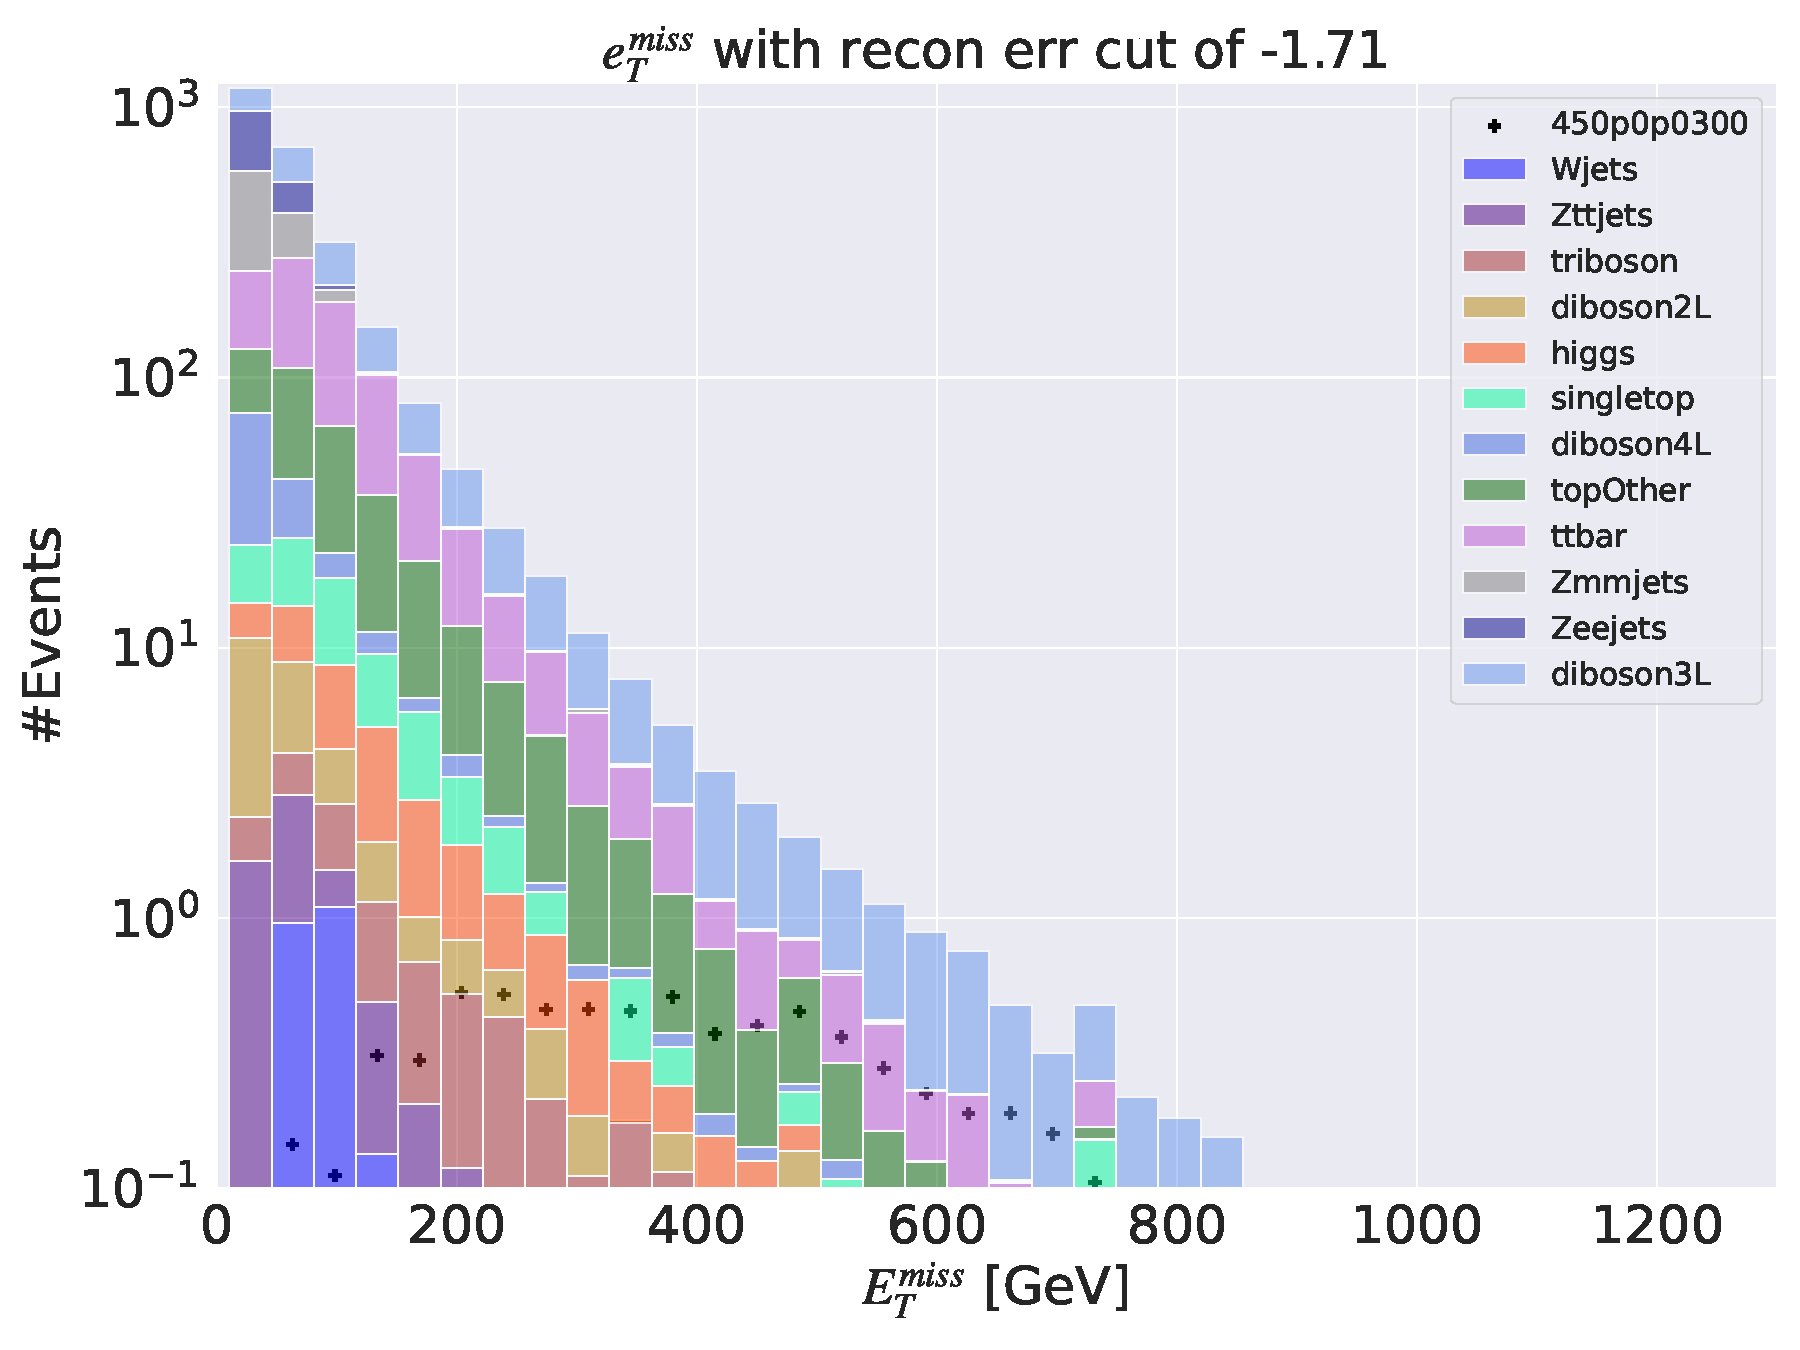
\includegraphics[width=\textwidth]{Figures/AE_testing/small/3lep/b_data_recon_big_rm3_feats_sig_450p0p0300_etmiss_recon_errcut_-1.71.pdf}
        \caption{}
        \label{fig:AE_3lep_small_etmiss_450}
    \end{subfigure}
    \hfill
    \begin{subfigure}{.49\textwidth}
        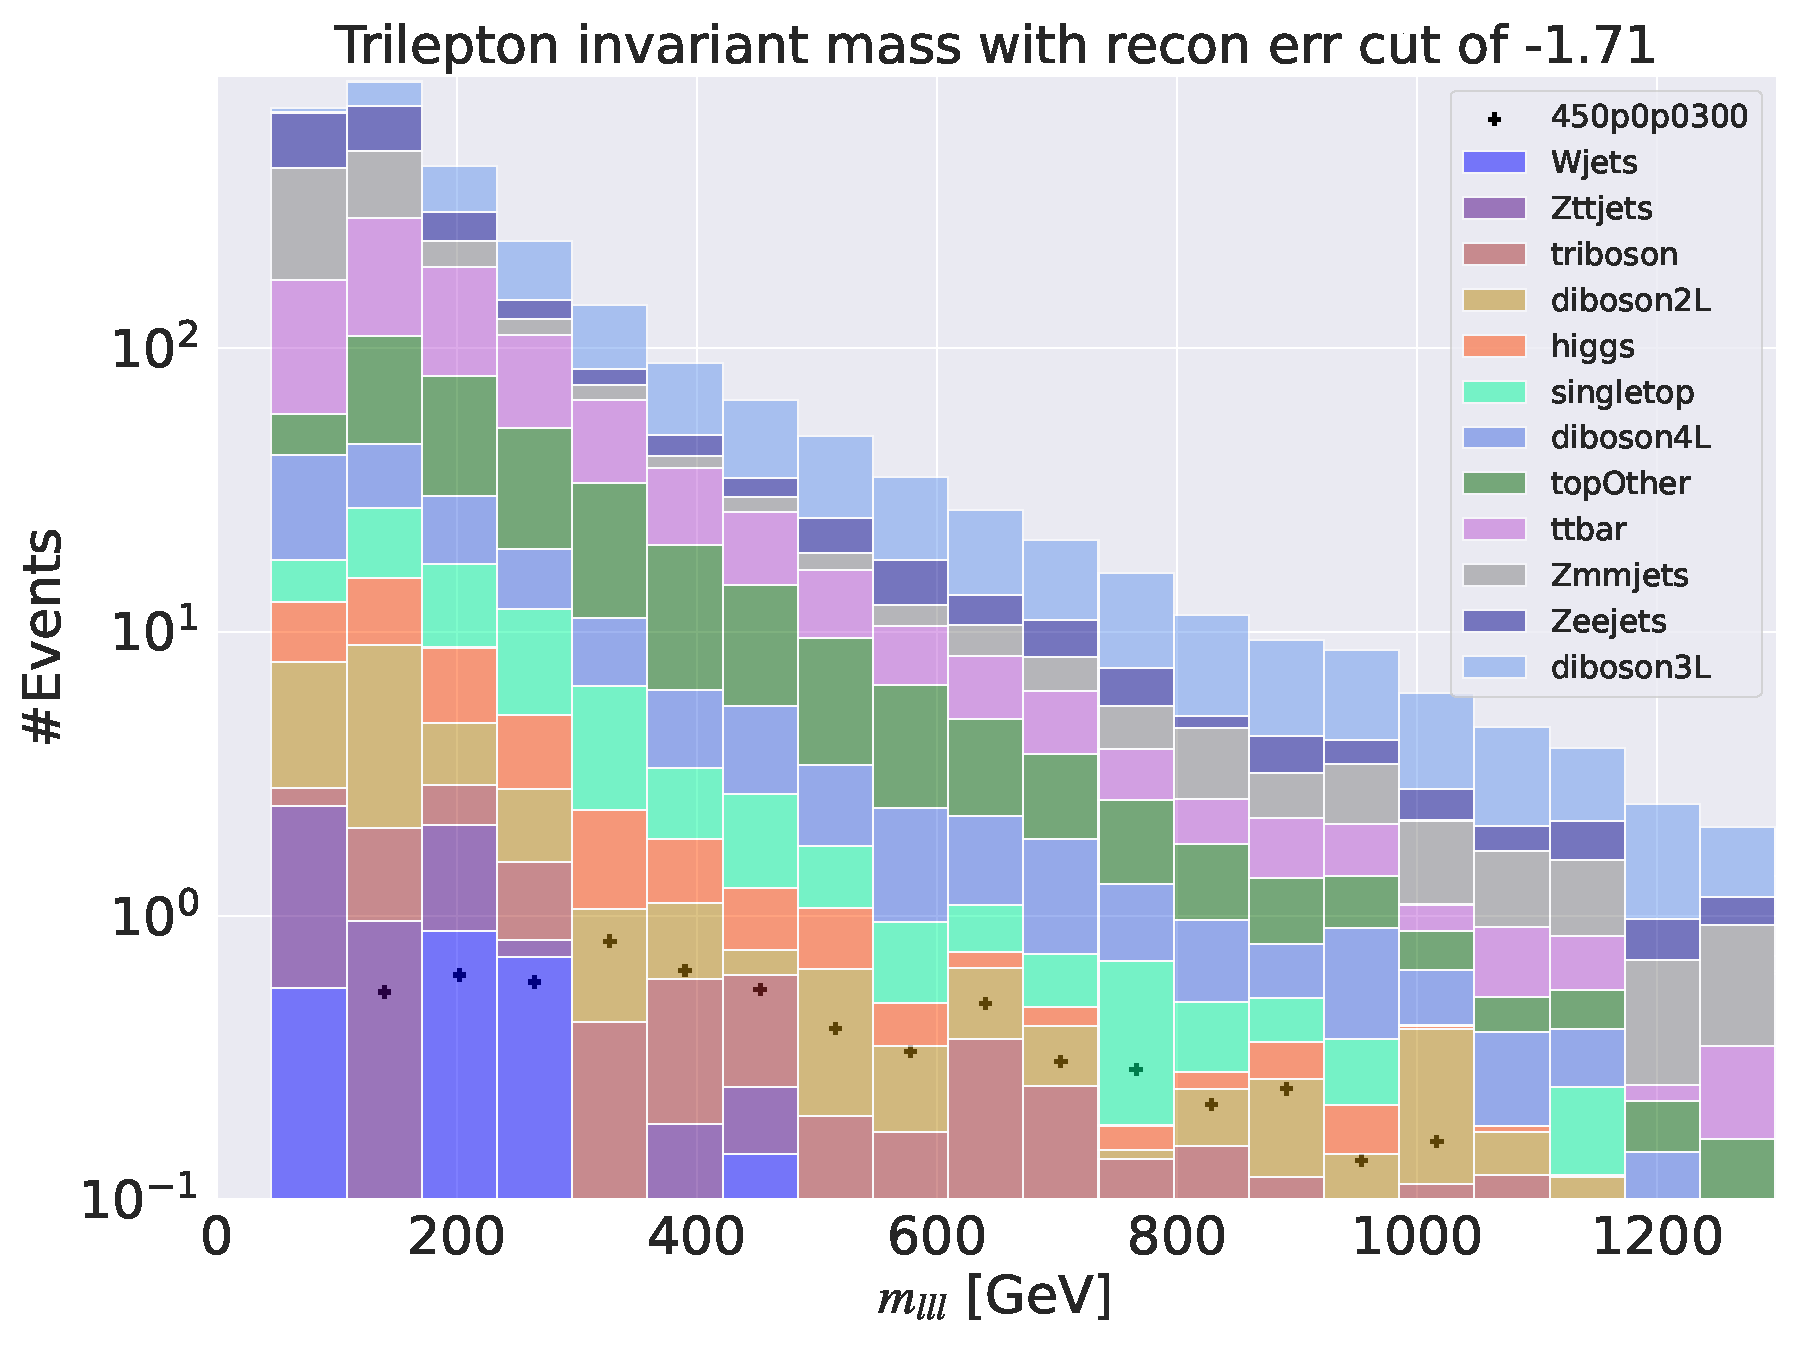
\includegraphics[width=\textwidth]{Figures/AE_testing/small/3lep/b_data_recon_big_rm3_feats_sig_450p0p0300_mlll_recon_errcut_-1.71.pdf}
        \caption{}
        \label{fig:AE_3lep_small_mlll_450}
    \end{subfigure}
    \hfill   
    \begin{subfigure}{.49\textwidth}
        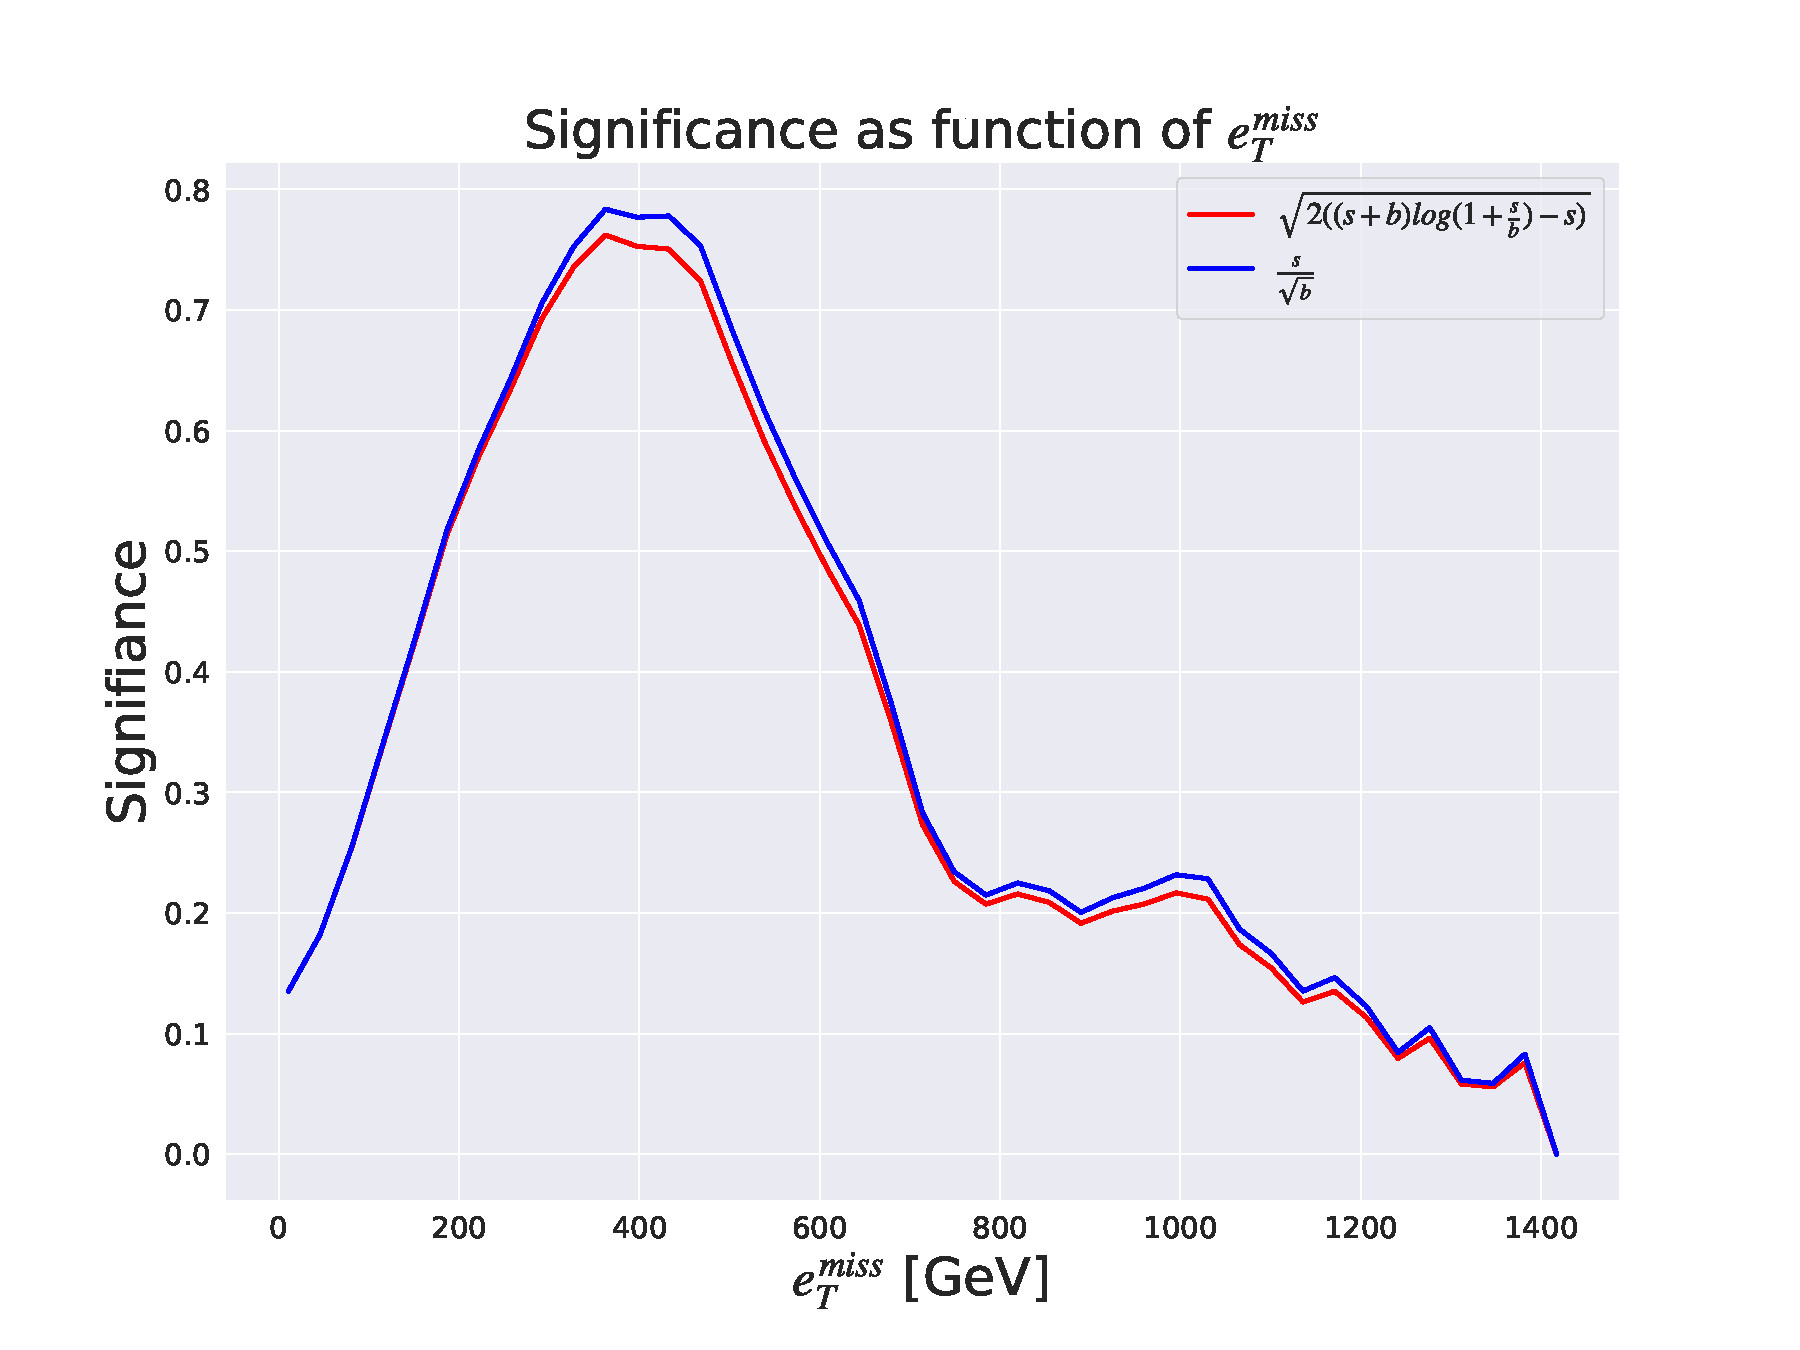
\includegraphics[width=\textwidth]{Figures/AE_testing/small/3lep/significance_etmiss_450p0p0300_-1.7067960296617328.pdf}
        \caption{}
        \label{fig:AE_3lep_small_signi_450}
    \end{subfigure}
    \hfill      
    \caption[3lep shallow network | $450p300$ | AE]{Reconstruction error, $e_T^{miss}$ signal region, $m_{lll}$ signal region and significance as function of 
    $e_T^{miss}$ for the shallow regular autoencoder using the SUSY $450p300$ model. Figure \ref{fig:AE_3lep_small_450} shows the reconstruction error 
    distribution for the SM MC and the SUSY signal. Here the autoencoder produces the same reconstruction error shape for both background and 
    signal, but with a small separation of the peaks of the distributions. Figure \ref{fig:AE_3lep_small_etmiss_450} shows the $e_T^{miss}$ 
    distribution for the SM MC and the SUSY signal in the signal region, defined as the region having a $log_{10}$ 
    reconstruction error above -1.71. Most of 
    the background is removed, and the peaks of the SM MC and signal distributions are somewhat separated. Figure 
    \ref{fig:AE_3lep_small_mlll_450} shows the $m_{lll}$ distribution for the SM MC and the SUSY signal. 
    The shape of the SM MC and the signal distributions are too similar to distinguish. Figure \ref{fig:AE_3lep_small_signi_450} shows the significance as 
    function of $e_T^{miss}$. The maximum significance is found when applying a cut of about > 380 GeV in the $e_T^{miss}$, with a significance of around $0.78$.}
    \label{fig:AE_3lep_small_rec_sig_signi_450}
\end{figure}








\begin{figure}[!htb]
    \centering
    \begin{subfigure}{.49\textwidth}
        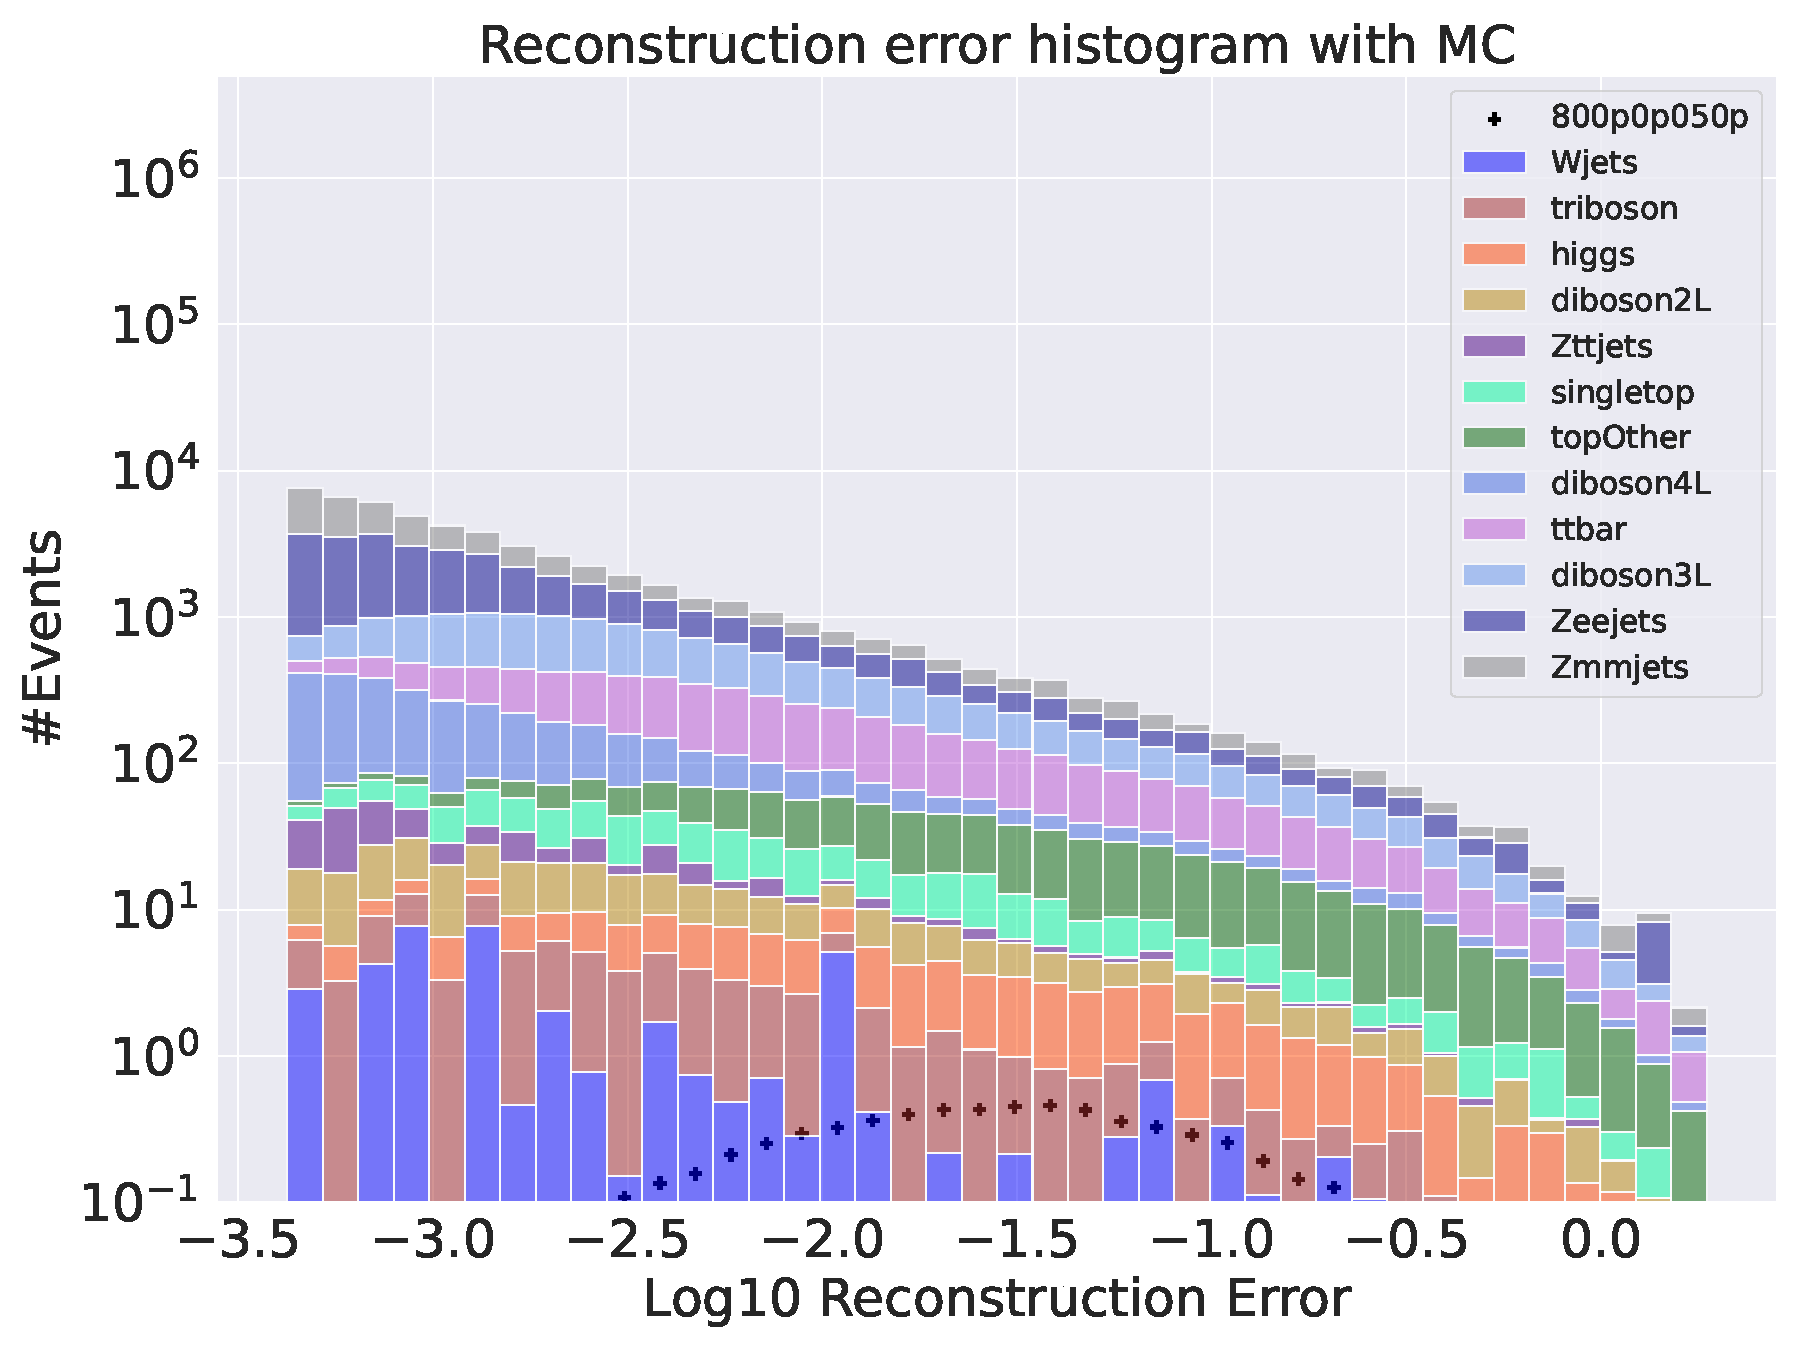
\includegraphics[width=\textwidth]{Figures/AE_testing/big/3lep/b_data_recon_big_rm3_feats_sig_800p0p050p.pdf}
        \caption{ }
        \label{fig:AE_3lep_big_800}
    \end{subfigure}
    \hfill
    \begin{subfigure}{.49\textwidth}
        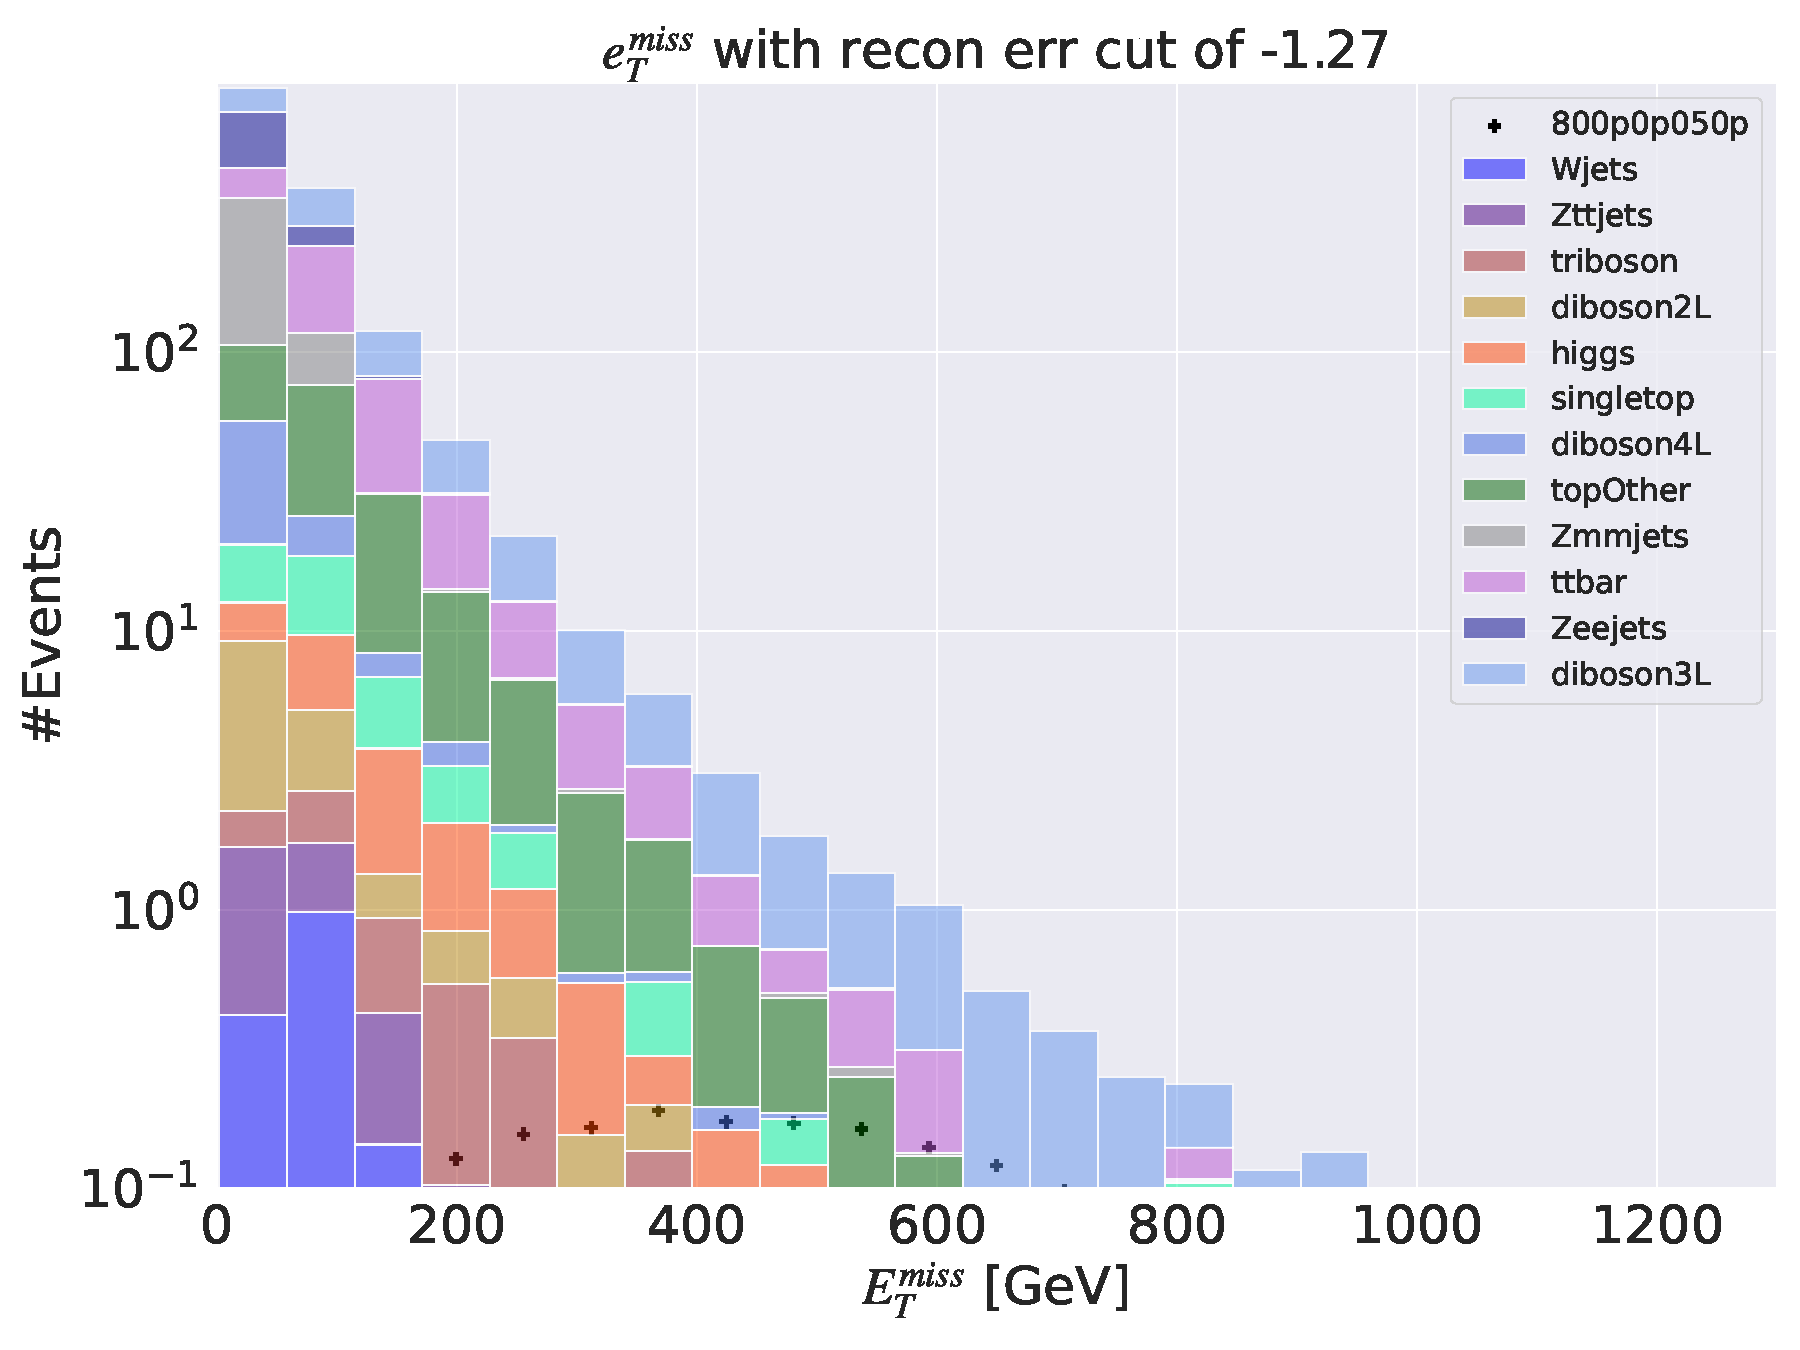
\includegraphics[width=\textwidth]{Figures/AE_testing/big/3lep/b_data_recon_big_rm3_feats_sig_800p0p050p_etmiss_recon_errcut_-1.27.pdf}
        \caption{}
        \label{fig:AE_3lep_big_etmiss_800}
    \end{subfigure}
    \hfill
    \begin{subfigure}{.49\textwidth}
        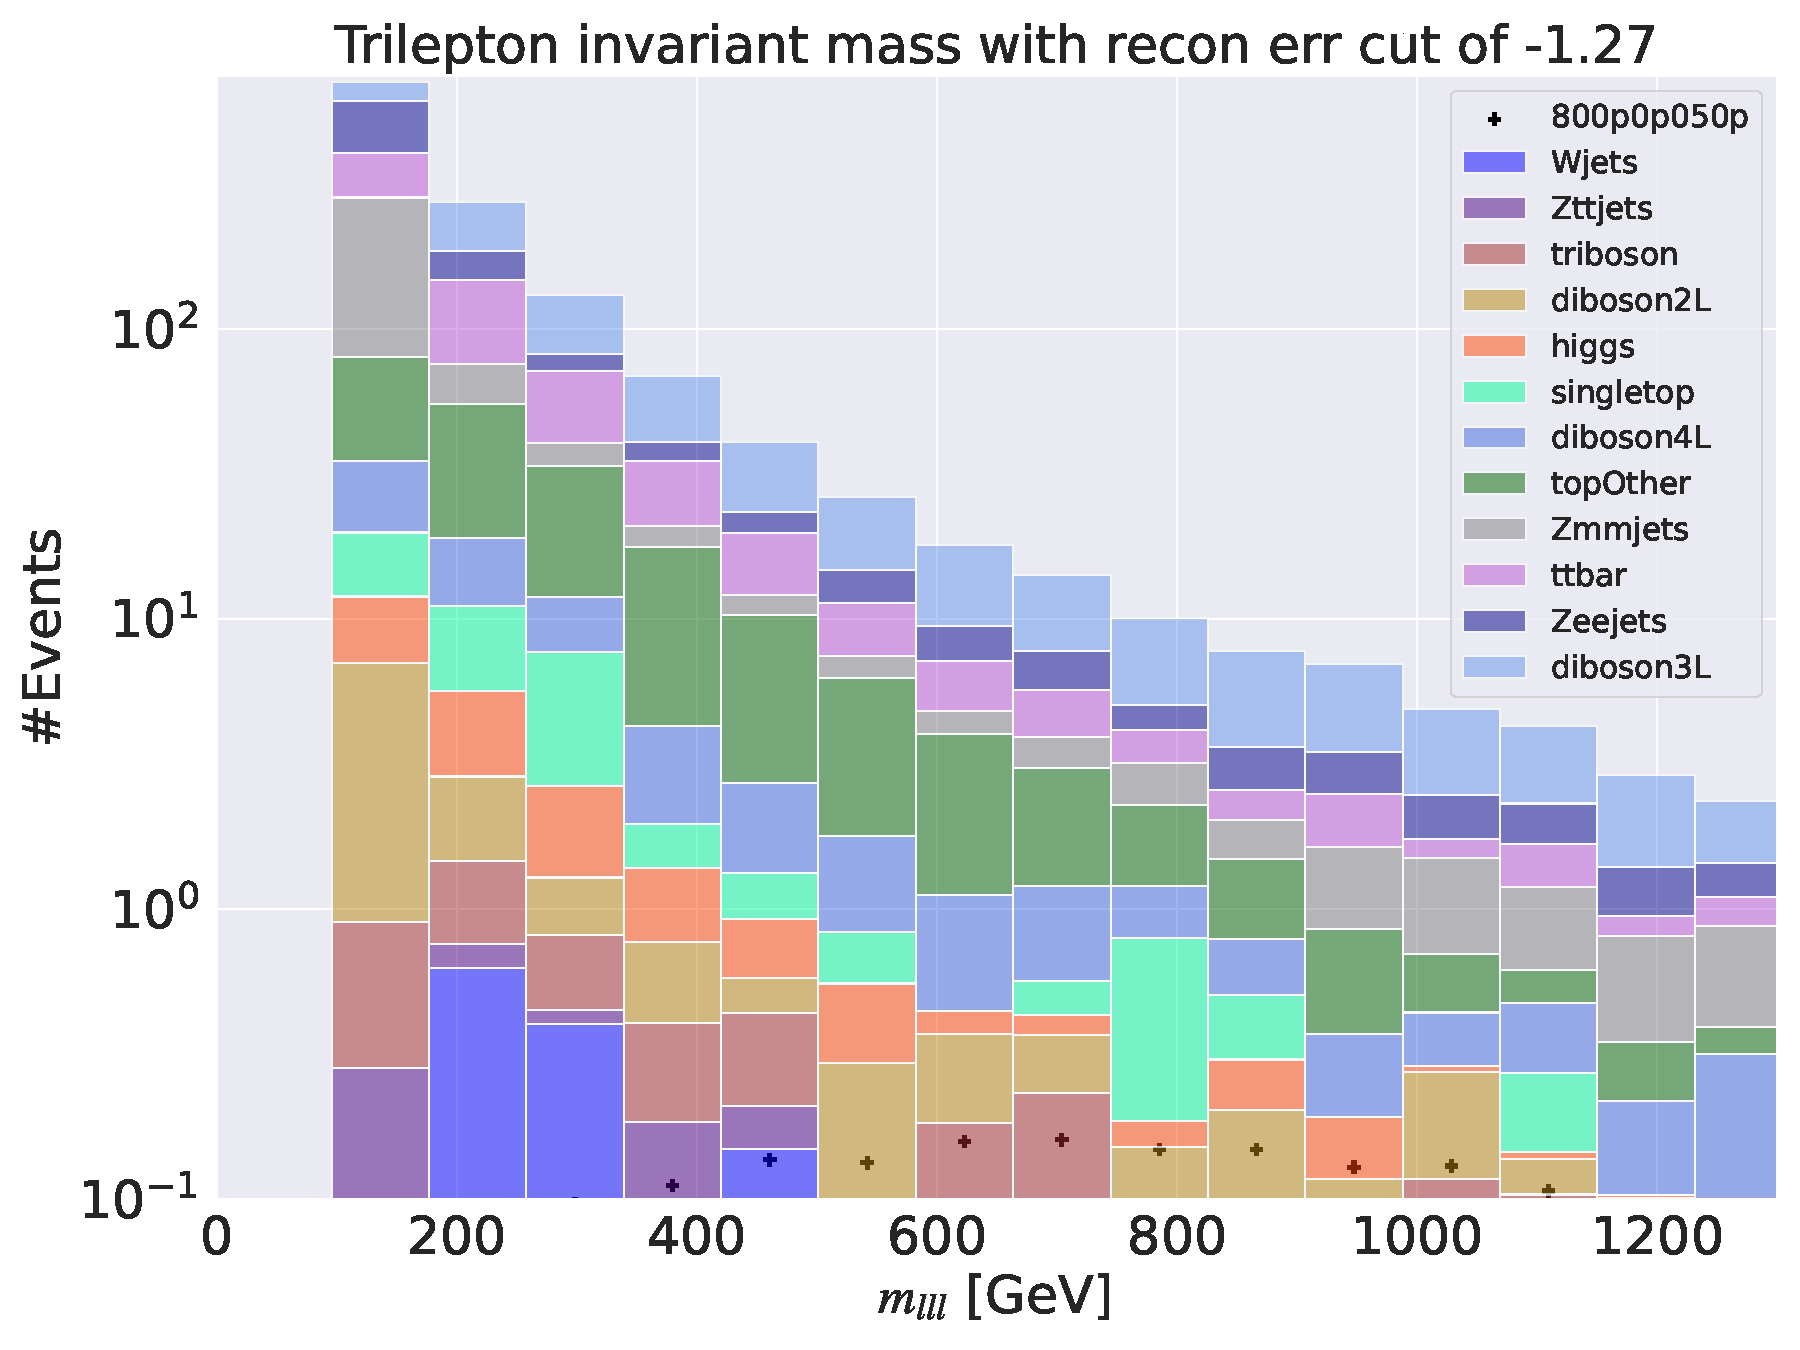
\includegraphics[width=\textwidth]{Figures/AE_testing/big/3lep/b_data_recon_big_rm3_feats_sig_800p0p050p_mlll_recon_errcut_-1.27.pdf}
        \caption{}
        \label{fig:AE_3lep_big_mlll_800}
    \end{subfigure}
    \hfill   
    \begin{subfigure}{.49\textwidth}
        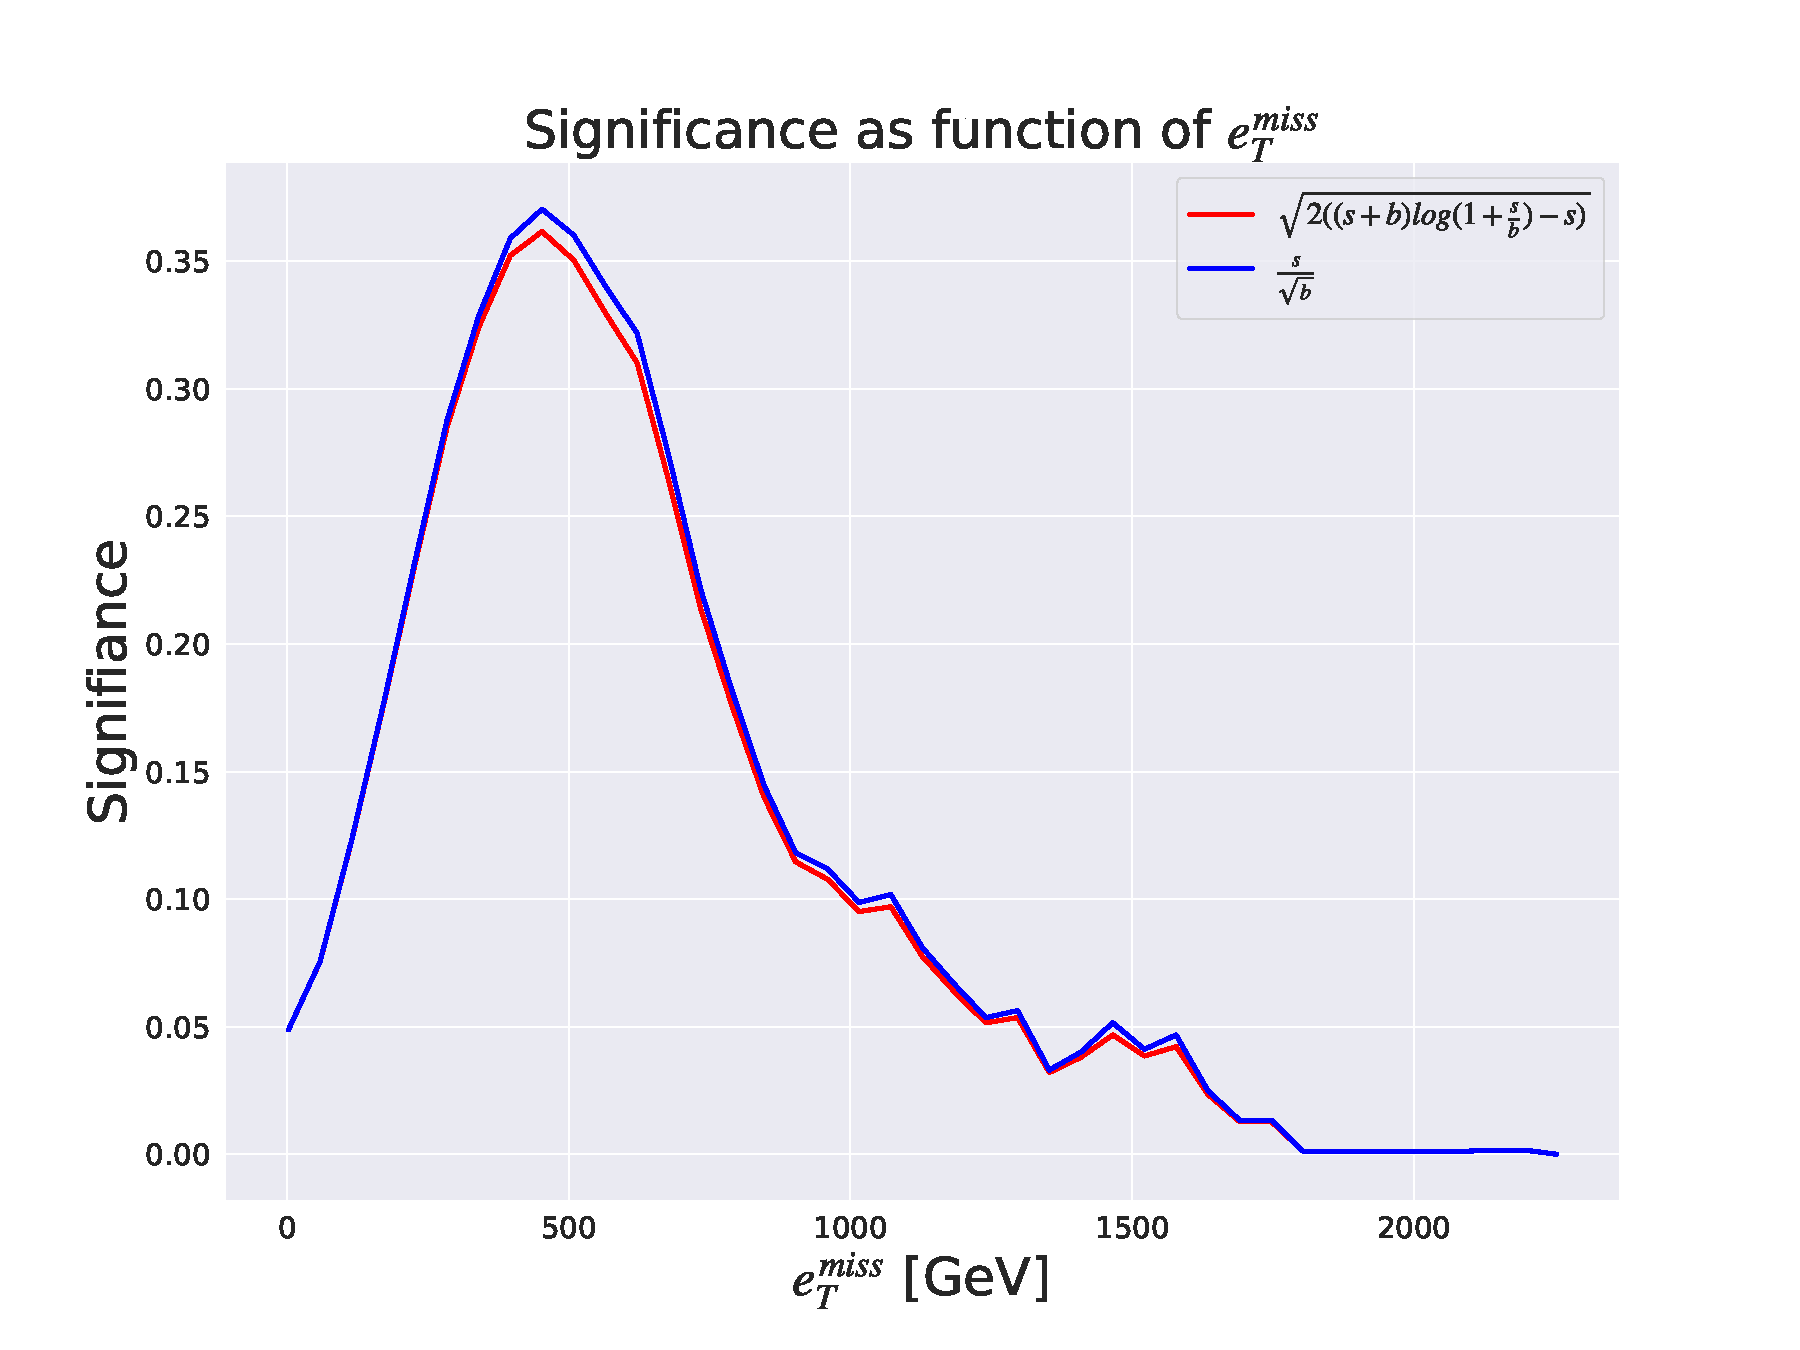
\includegraphics[width=\textwidth]{Figures/AE_testing/big/3lep/significance_etmiss_800p0p050p_-1.2726592563014343.pdf}
        \caption{}
        \label{fig:AE_3lep_big_signi_800}
    \end{subfigure}
    \hfill      
    \caption[3lep deep network | $800p50$ | AE]{Reconstruction error, $e_T^{miss}$ signal region, $m_{lll}$ signal region and significance as function of 
    $e_T^{miss}$ for the deep regular autoencoder using the SUSY $800p50$. 
    Figure \ref{fig:AE_3lep_big_800} shows the reconstruction error 
    distribution for the SM MC and the SUSY signal. Here the autoencoder produces a mirrored reconstruction error shape for background and 
    signal. The peaks of the two distributions are separated with two orders of magnitude in reconstruction error. Figure \ref{fig:AE_3lep_big_etmiss_800} 
    shows the $e_T^{miss}$ distribution for the SM MC and the SUSY signal in the signal region, defined as the region 
    having a $log_{10}$ reconstruction error above -1.27. Most of the background is removed, and the peaks of the SM MC and signal 
    distributions are separated. Figure \ref{fig:AE_3lep_big_mlll_800} shows the $m_{lll}$ distribution for the SM MC and the SUSY signal. 
    The shape of the SM MC and the signal distributions are somewhat separated. Figure \ref{fig:AE_3lep_big_signi_800} shows the significance as function of
    $e_T^{miss}$. The maximum significance is found when applying a cut of about > 430 GeV in the $e_T^{miss}$, with a significance of around $0.37$.}
    \label{fig:AE_3lep_big_rec_sig_signi_800}
\end{figure}

\begin{figure}[!htb]
    \centering
    \begin{subfigure}{.49\textwidth}
        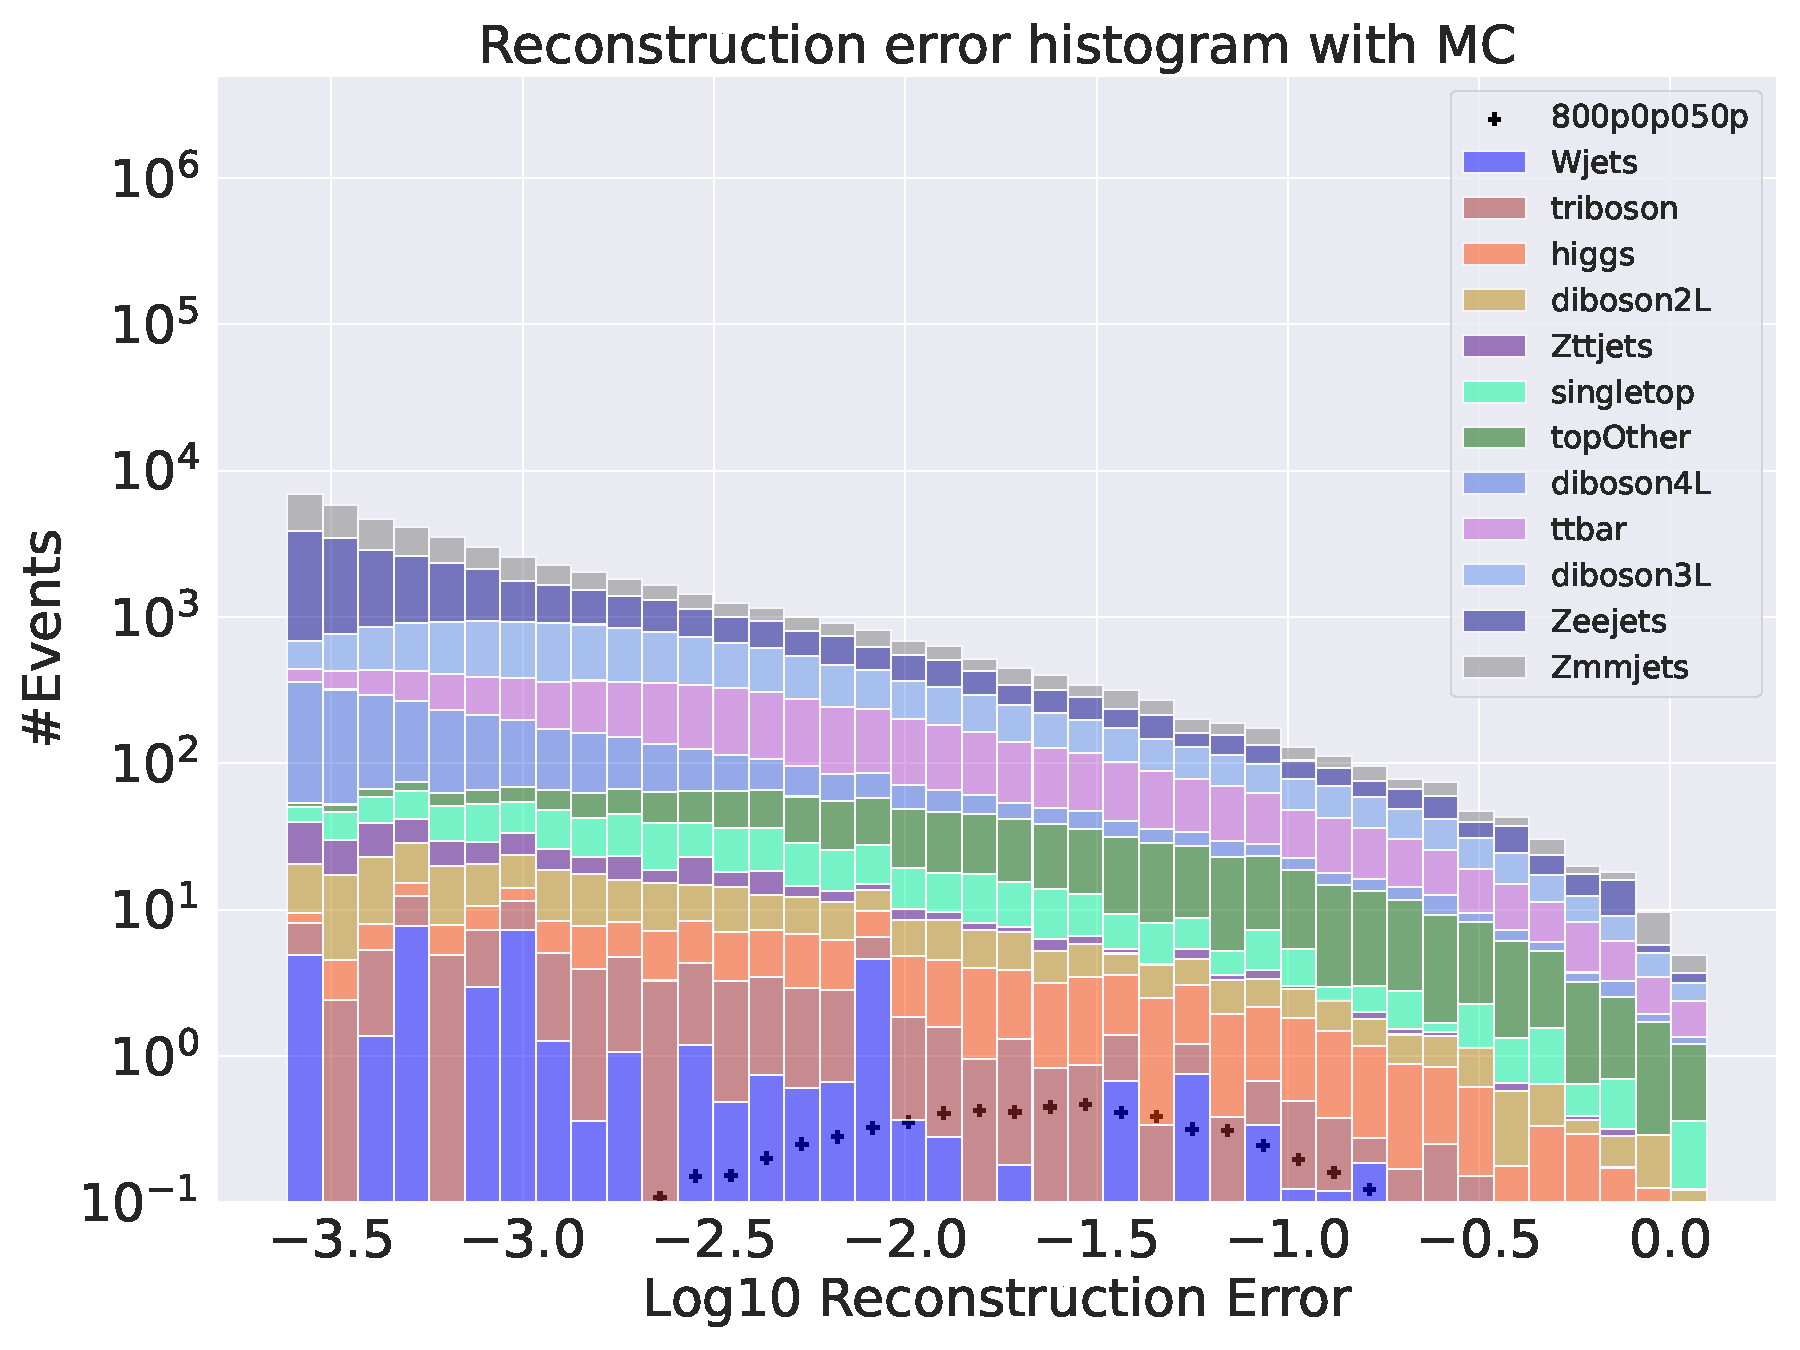
\includegraphics[width=\textwidth]{Figures/AE_testing/small/3lep/b_data_recon_big_rm3_feats_sig_800p0p050p.pdf}
        \caption{ }
        \label{fig:AE_3lep_small_800}
    \end{subfigure}
    \hfill
    \begin{subfigure}{.49\textwidth}
        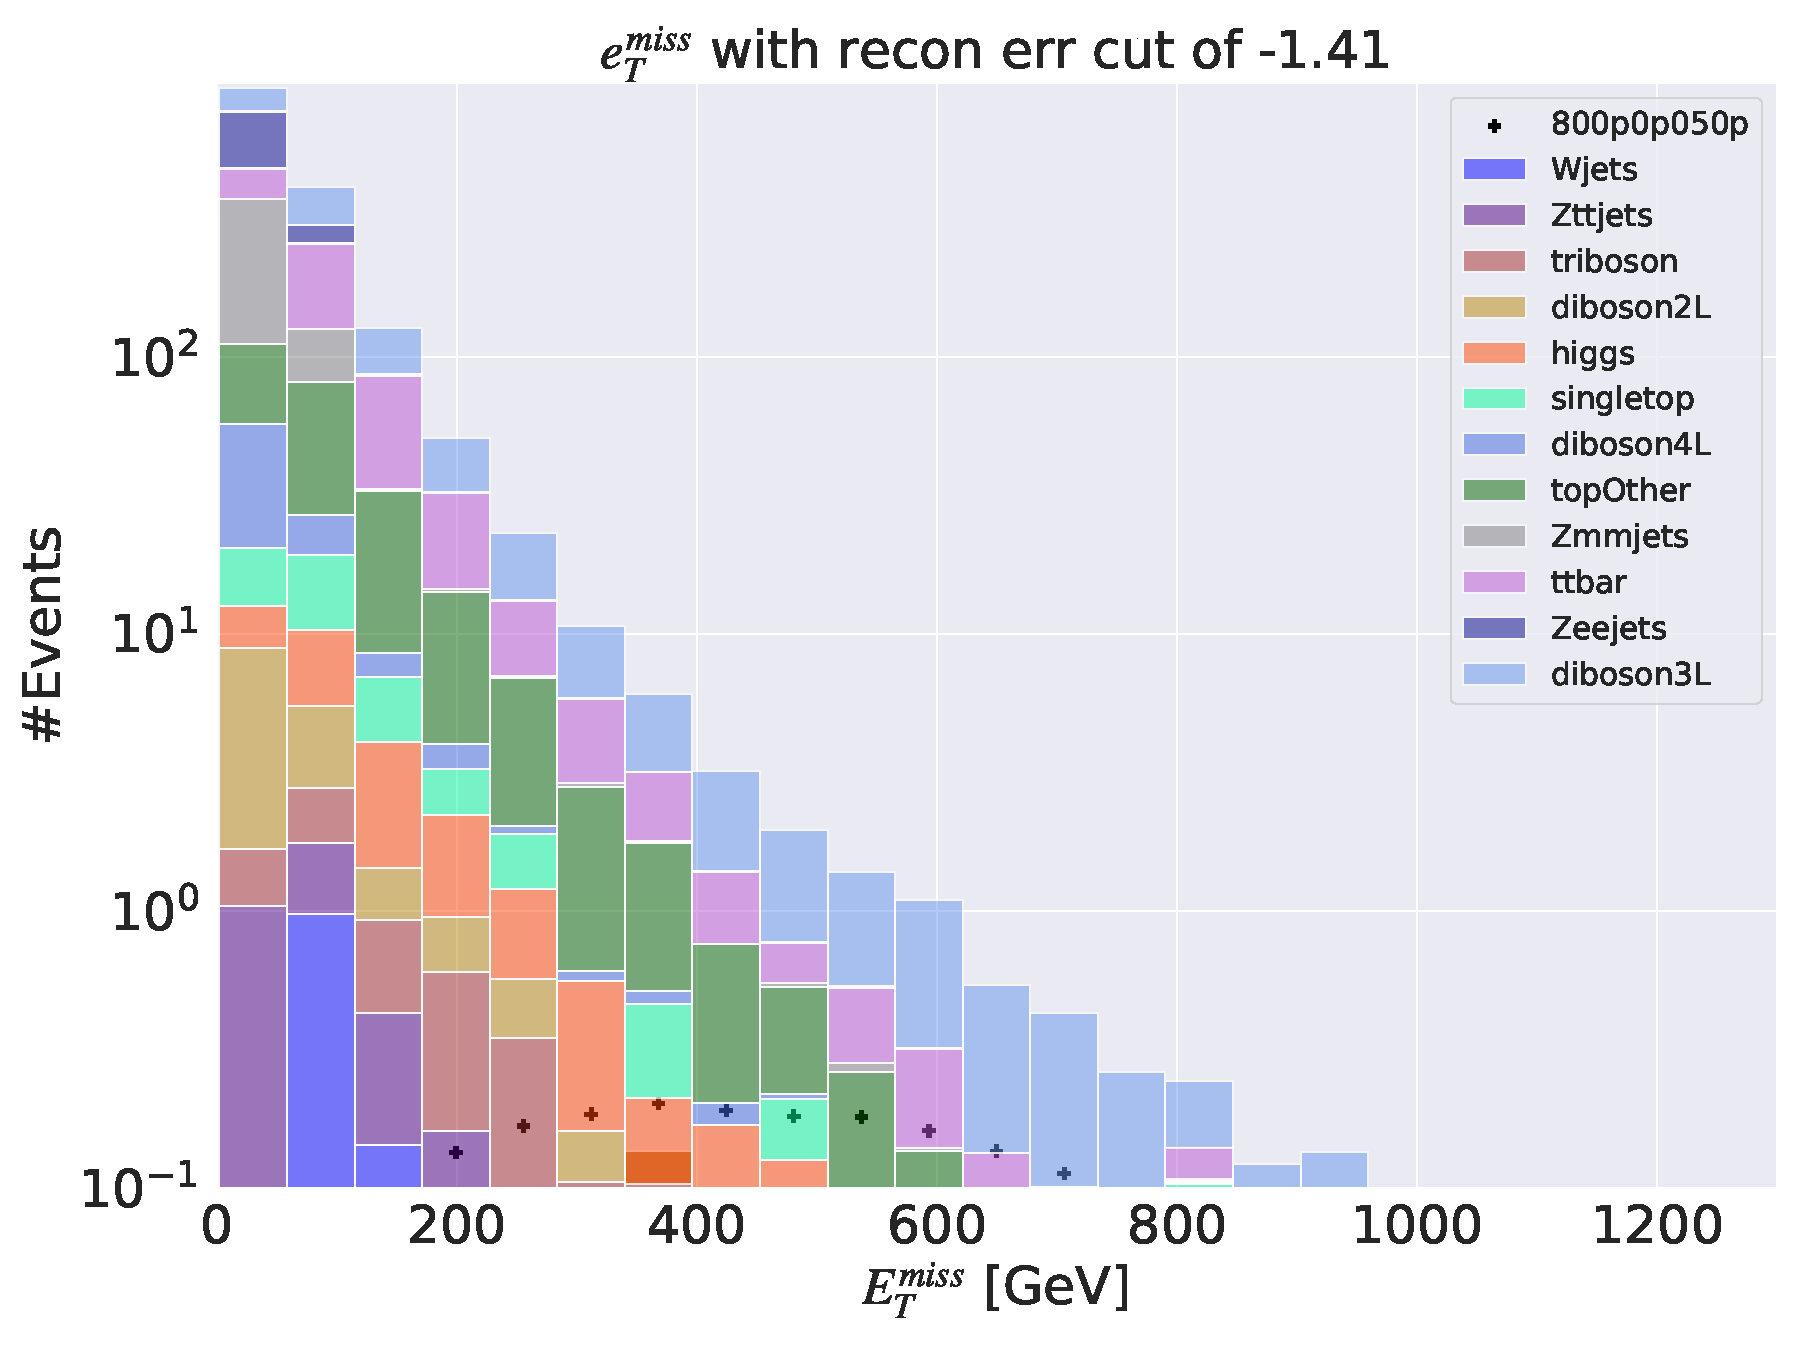
\includegraphics[width=\textwidth]{Figures/AE_testing/small/3lep/b_data_recon_big_rm3_feats_sig_800p0p050p_etmiss_recon_errcut_-1.41.pdf}
        \caption{}
        \label{fig:AE_3lep_small_etmiss_800}
    \end{subfigure}
    \hfill
    \begin{subfigure}{.49\textwidth}
        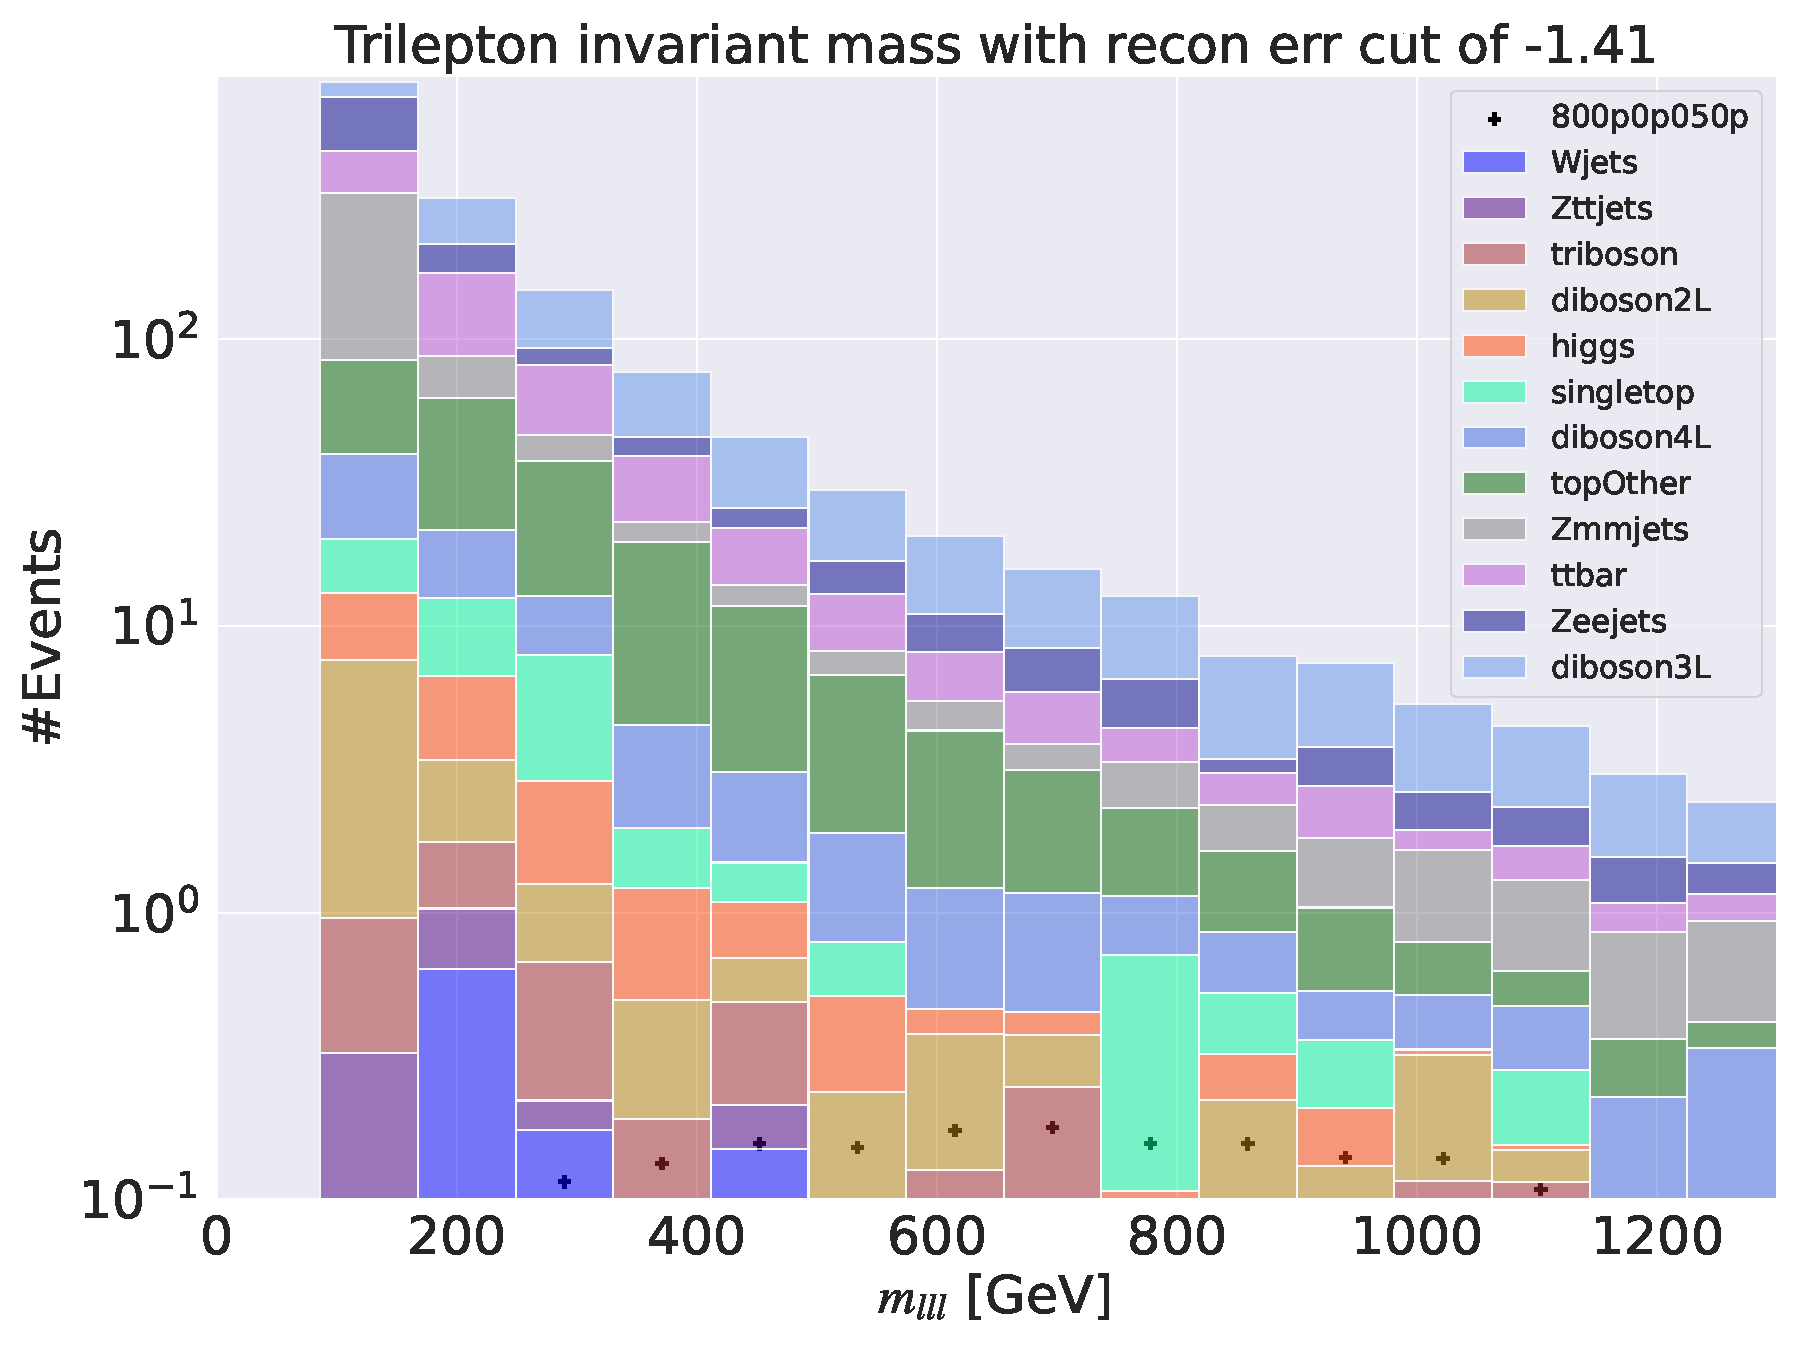
\includegraphics[width=\textwidth]{Figures/AE_testing/small/3lep/b_data_recon_big_rm3_feats_sig_800p0p050p_mlll_recon_errcut_-1.41.pdf}
        \caption{}
        \label{fig:AE_3lep_small_mlll_800}
    \end{subfigure}
    \hfill   
    \begin{subfigure}{.49\textwidth}
        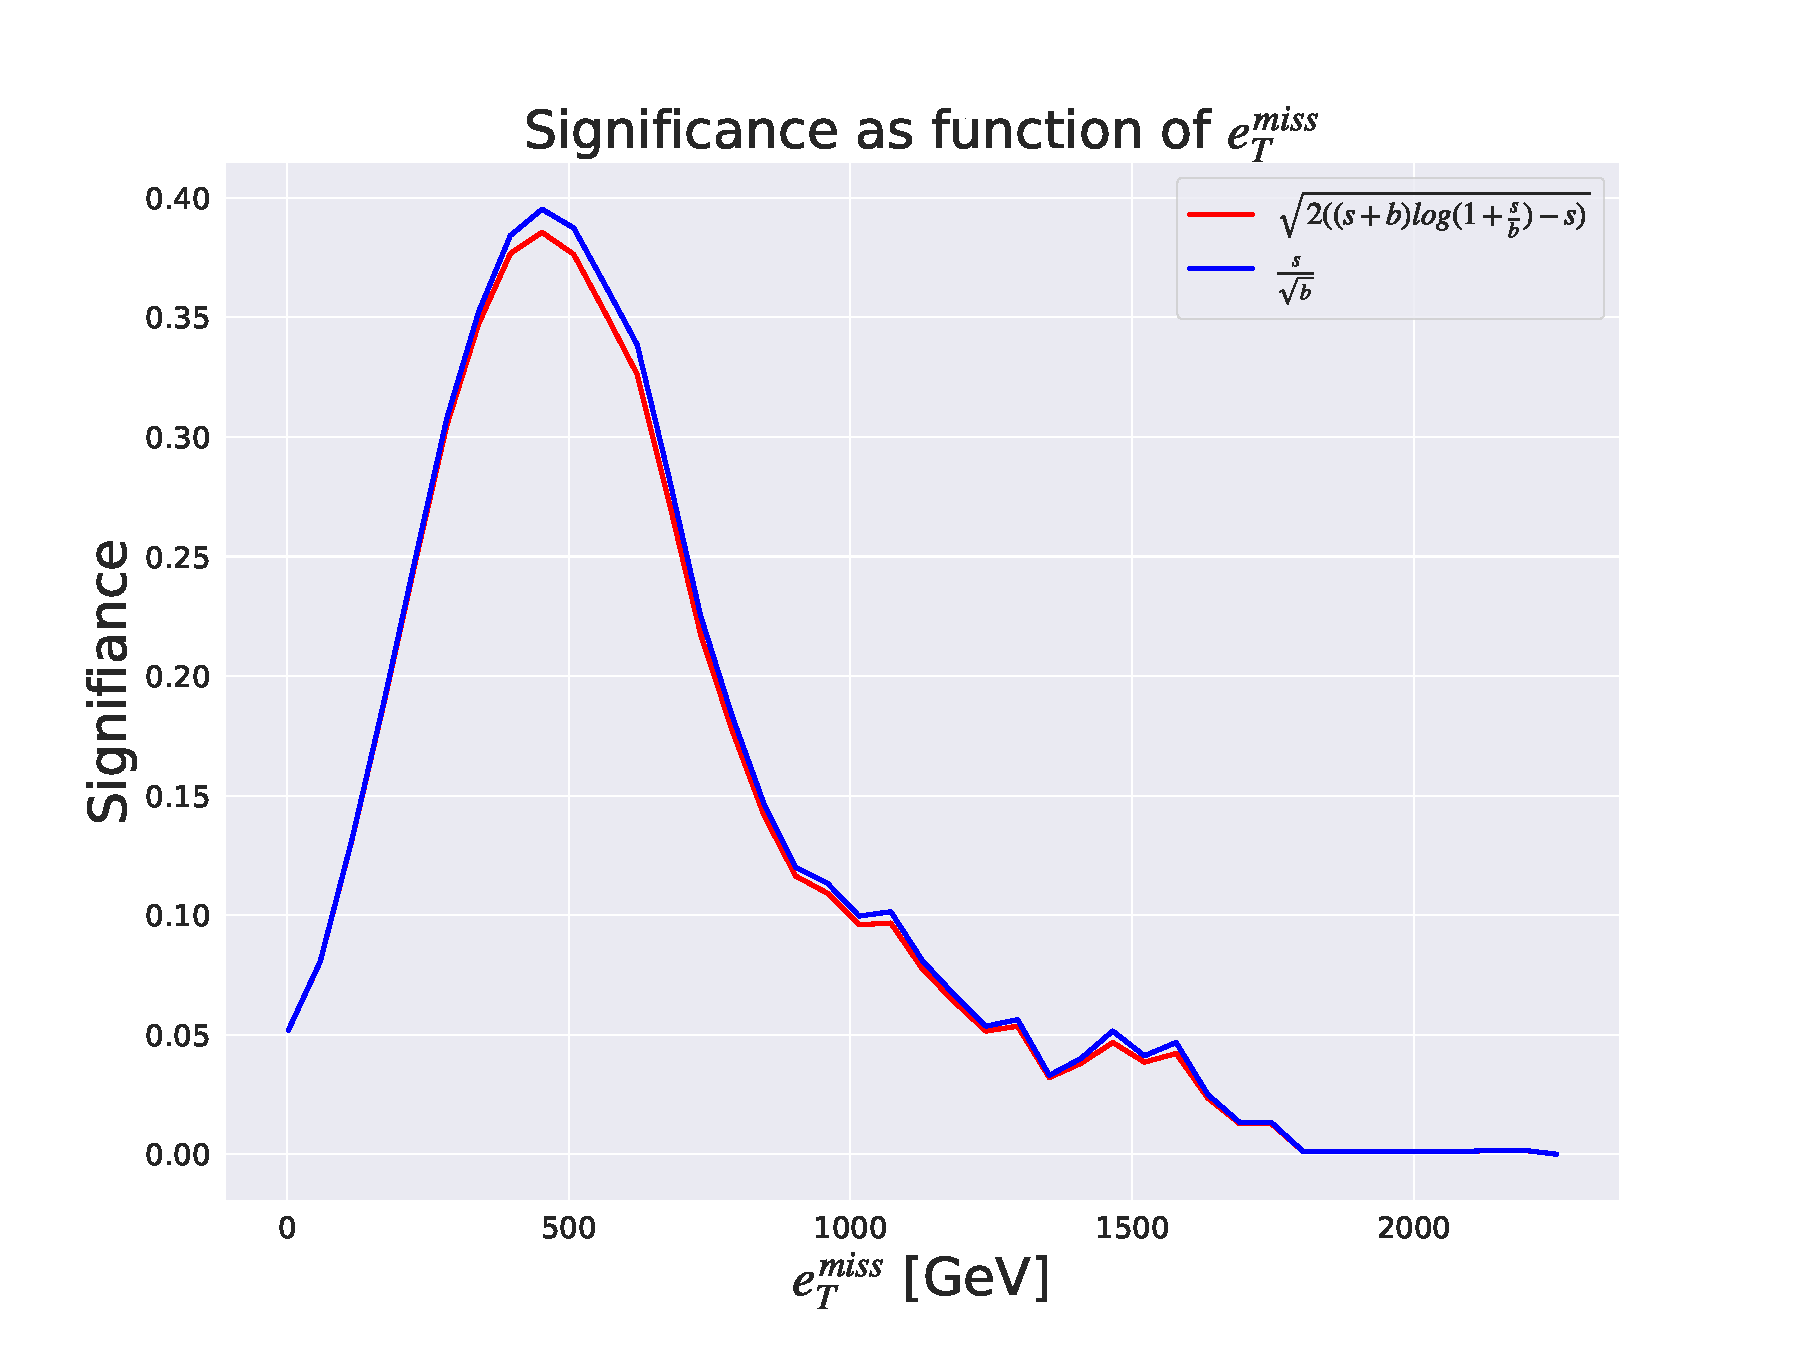
\includegraphics[width=\textwidth]{Figures/AE_testing/small/3lep/significance_etmiss_800p0p050p_-1.4089386402528896.pdf}
        \caption{}
        \label{fig:AE_3lep_small_signi_800}
    \end{subfigure}
    \hfill      
    \caption[3lep shallow network | $800p50$ | AE]{Reconstruction error, $e_T^{miss}$ signal region, $m_{lll}$ signal region and significance as function of 
    $e_T^{miss}$ for the shallow regular autoencoder using the SUSY $800p50$. 
    Figure \ref{fig:AE_3lep_small_800} shows the reconstruction error 
    distribution for the SM MC and the SUSY signal. Here the autoencoder produces a mirrored reconstruction error shape for background and 
    signal. The peaks of the two distributions are separated with two orders of magnitude in reconstruction error. Figure \ref{fig:AE_3lep_small_etmiss_800} 
    shows the $e_T^{miss}$ distribution for the SM MC and the SUSY signal in the signal region, defined as the region having a $log_{10}$ reconstruction error above -1.41 Most of the background is removed, and the peaks of the SM MC and signal 
    distributions are separated. Figure \ref{fig:AE_3lep_small_mlll_800} shows the $m_{lll}$ distribution for the SM MC and the SUSY signal. 
    The shape of the SM MC and the signal distributions are somewhat separated. Figure \ref{fig:AE_3lep_small_signi_800} shows the significance as function of
    $e_T^{miss}$. The maximum significance is found when applying a cut of about > 450 GeV in the $e_T^{miss}$, with a significance of around $0.39$.}
    \label{fig:AE_3lep_small_rec_sig_signi_800}
\end{figure}

Figures \ref{fig:AE_3lep_big_rec_sig_signi_450}, \ref{fig:AE_3lep_small_rec_sig_signi_450}, 
\ref{fig:AE_3lep_big_rec_sig_signi_800} and \ref{fig:AE_3lep_small_rec_sig_signi_800} contain four 
subplots each showing the total reconstruction error distributions (a), the $e_T^{miss}$ signal regions (b), 
the $m_{lll}$ signal regions (c) and the significances as function of a lower cut on $e_T^{miss}$ curve (d) 
for the shallow (figure \ref{fig:AE_3lep_small_rec_sig_signi_450} and \ref{fig:AE_3lep_small_rec_sig_signi_800}) 
and deep (figure \ref{fig:AE_3lep_big_rec_sig_signi_450} and \ref{fig:AE_3lep_big_rec_sig_signi_800}) regular autoencoder
using two different SUSY scenarios for inference. 
From figures \ref{fig:AE_3lep_big_450} - \ref{fig:AE_3lep_small_800} it is clear that the 
autoencoders struggles more to reconstruct the $800p50$ point (i.e. more anomalous, higher reconstruction error) 
compared with the $450p300$ point, which is expected from the fact that the $800p50$ point has a larger 
mass difference between the chargino and the lightest supersymetric particle and thus would lead to more missing 
transverse energy in the events. The steepness of the 
slopes of the reconstruction error show quite similar behavior for both the shallow and deep regular autoencoders, 
indicating that the performance of these two models does not differ. 
The bulk of the events are below $10^{-2}$ reconstruction error, indicating that the autoencoder 
has learned a lot of the internal RMM structures for the 3 lepton + $e_T^{miss}$ final state MC. \par
In figures \ref{fig:AE_3lep_big_etmiss_450}, \ref{fig:AE_3lep_small_etmiss_450}, 
\ref{fig:AE_3lep_big_etmiss_800} and  \ref{fig:AE_3lep_small_etmiss_800} signal regions 
are created for each of the two SUSY models for both the shallow and deep regular autoencoder. The cuts 
were created using the median and then iteratively increasing the error requirement, as 
explained in section \ref{sec:strategy}. Only one of the three cuts done are shown here, the 
rest can be found in appendix \ref{sec:app3}. The most inclusive signal region is chosen in order to 
illustrate the difficulty of the anomaly detction method since we do not have 
any idea how anomalous (i.e. how large reconstruction error) we expect a BSM signal to have. 
A too strict a cut could possibly eliminate a large fraction of the 
signal events in the signal region, whereas a too loose a cut would result in the SM MC background dominating completely. \par
In figures \ref{fig:AE_3lep_big_mlll_450}, \ref{fig:AE_3lep_small_mlll_450}, \ref{fig:AE_3lep_big_mlll_800} and  
\ref{fig:AE_3lep_small_mlll_800} the $m_{lll}$ distributions for the most inclusive signal 
regions from both the shallow and deep regular 
autoencoder for both of the SUSY signals. The results from the most inclusive signal region is shown here 
while the rest can be found in appendix \ref{sec:app3}. 
The difference observed in the $m_{lll}$ distribution between the SM MC and signal are small for both the 
shallow and deep autoencoders. This is expected considering the signal modeling being used, 
which do not have any particular resonance in the three-lepton invariant mass. \par 
In figures \ref{fig:AE_3lep_big_signi_450}, \ref{fig:AE_3lep_small_signi_450}, \ref{fig:AE_3lep_big_signi_800} and  
\ref{fig:AE_3lep_small_signi_800} the significance as a function of applying a lower cut on $e_T^{miss}$ is shown. 
It displays that an additional cut on $e_T^{miss}$ leads to an increased significance. The best case is achieved for 
the SUSY $450p300$ signal using the shallow autoencoder, leading to a significance of $0.78$.
Although the autoencoders gave a larger reconstruction error for the high-mass SUSY signal the final significance 
is found to be higher for the low mass SUSY signal. This is due to the cross section being a factor of 15 larger 
for the $450p300$ model compared with the $800p50$ model.


\subsubsection*{Variational autoencoder output}\label{sec:3lep_var}


\begin{figure}[!htb]
    \centering
    \begin{subfigure}{.49\textwidth}
        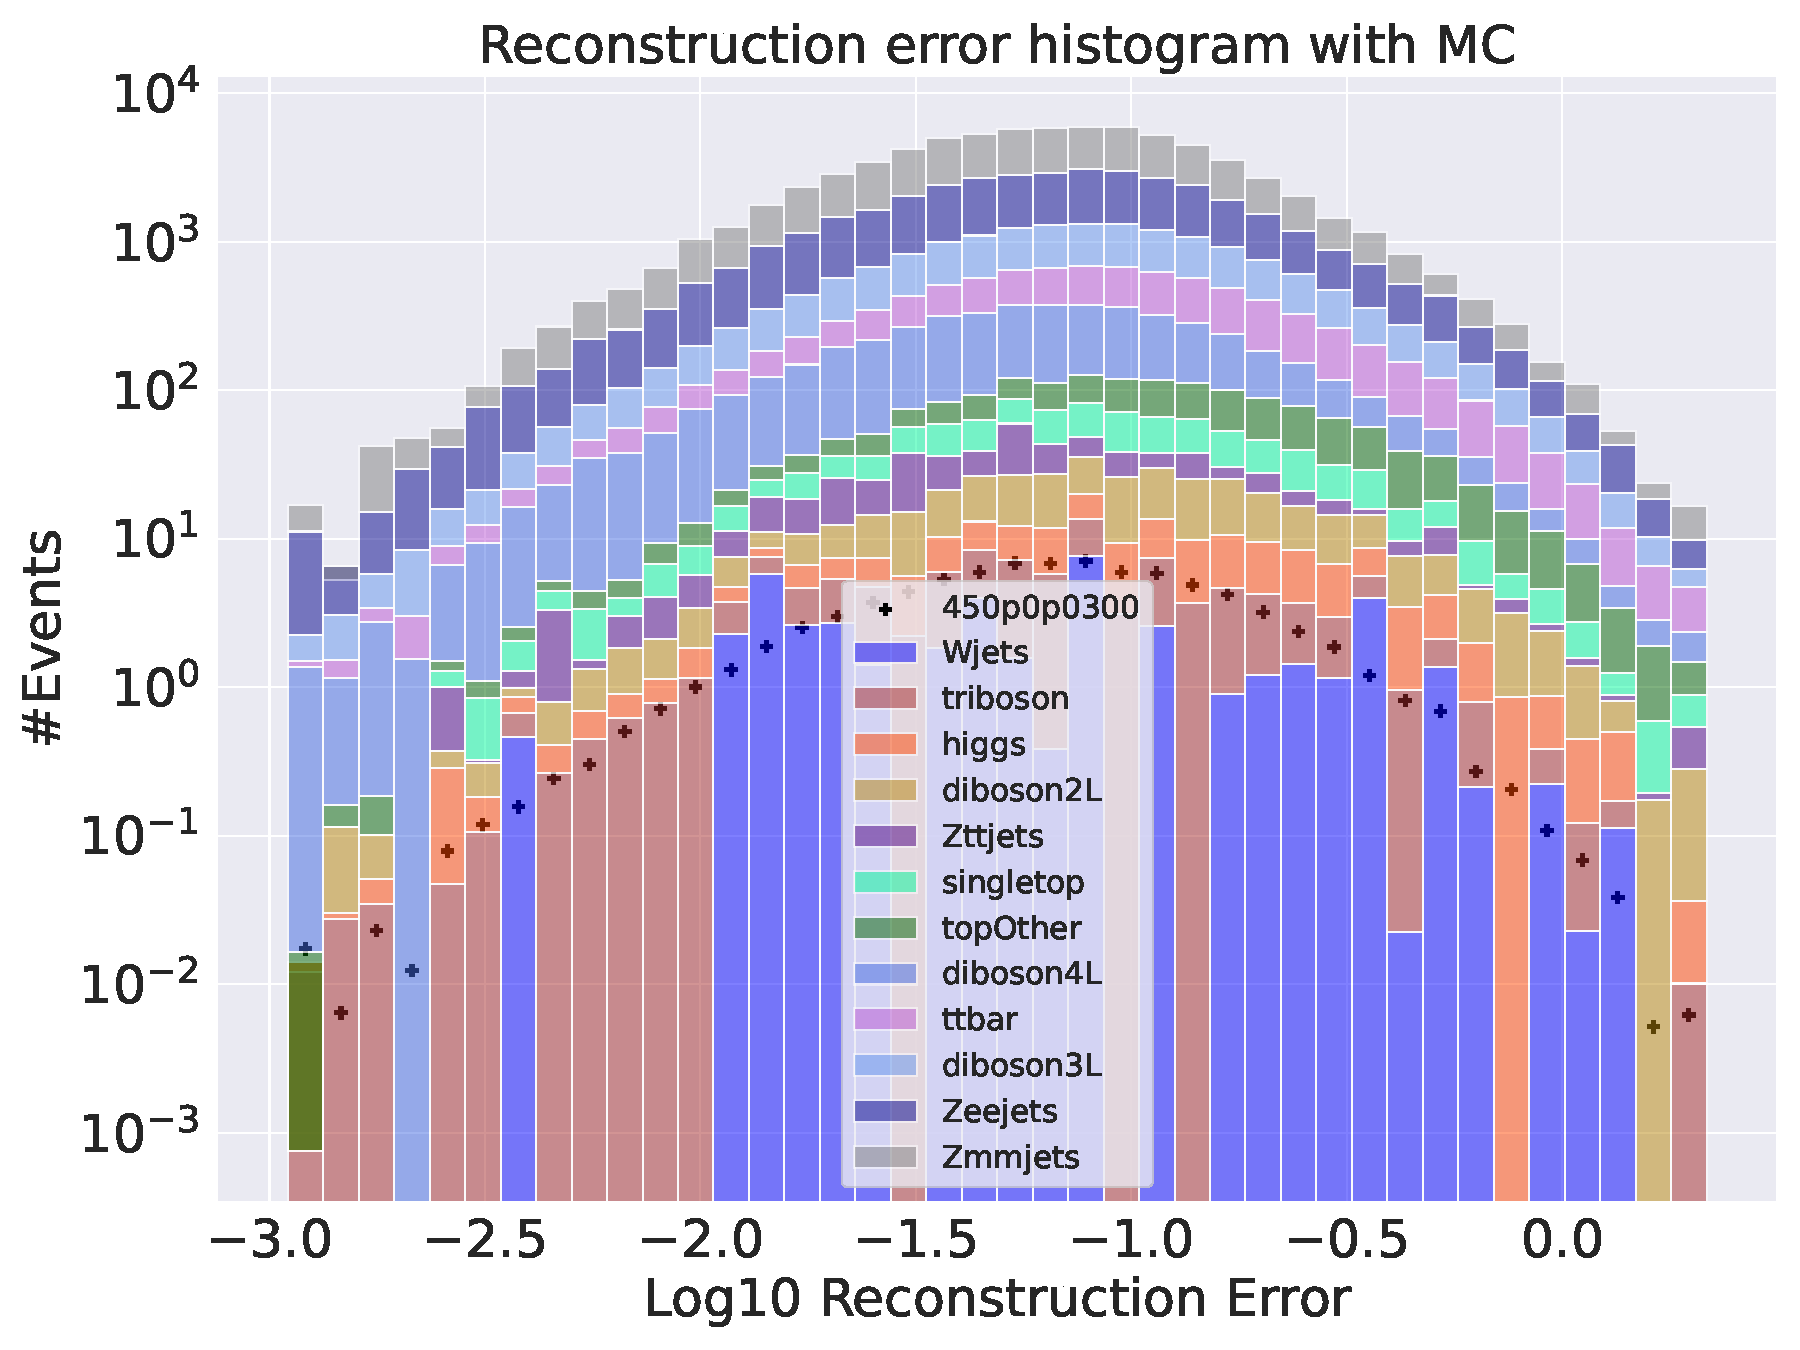
\includegraphics[width=\textwidth]{Figures/VAE_testing/big/3lep/b_data_recon_big_rm3_feats_sig_450p0p0300.pdf}
        \caption{ }
        \label{fig:VAE_3lep_big_450}
    \end{subfigure}
    \hfill
    \begin{subfigure}{.49\textwidth}
        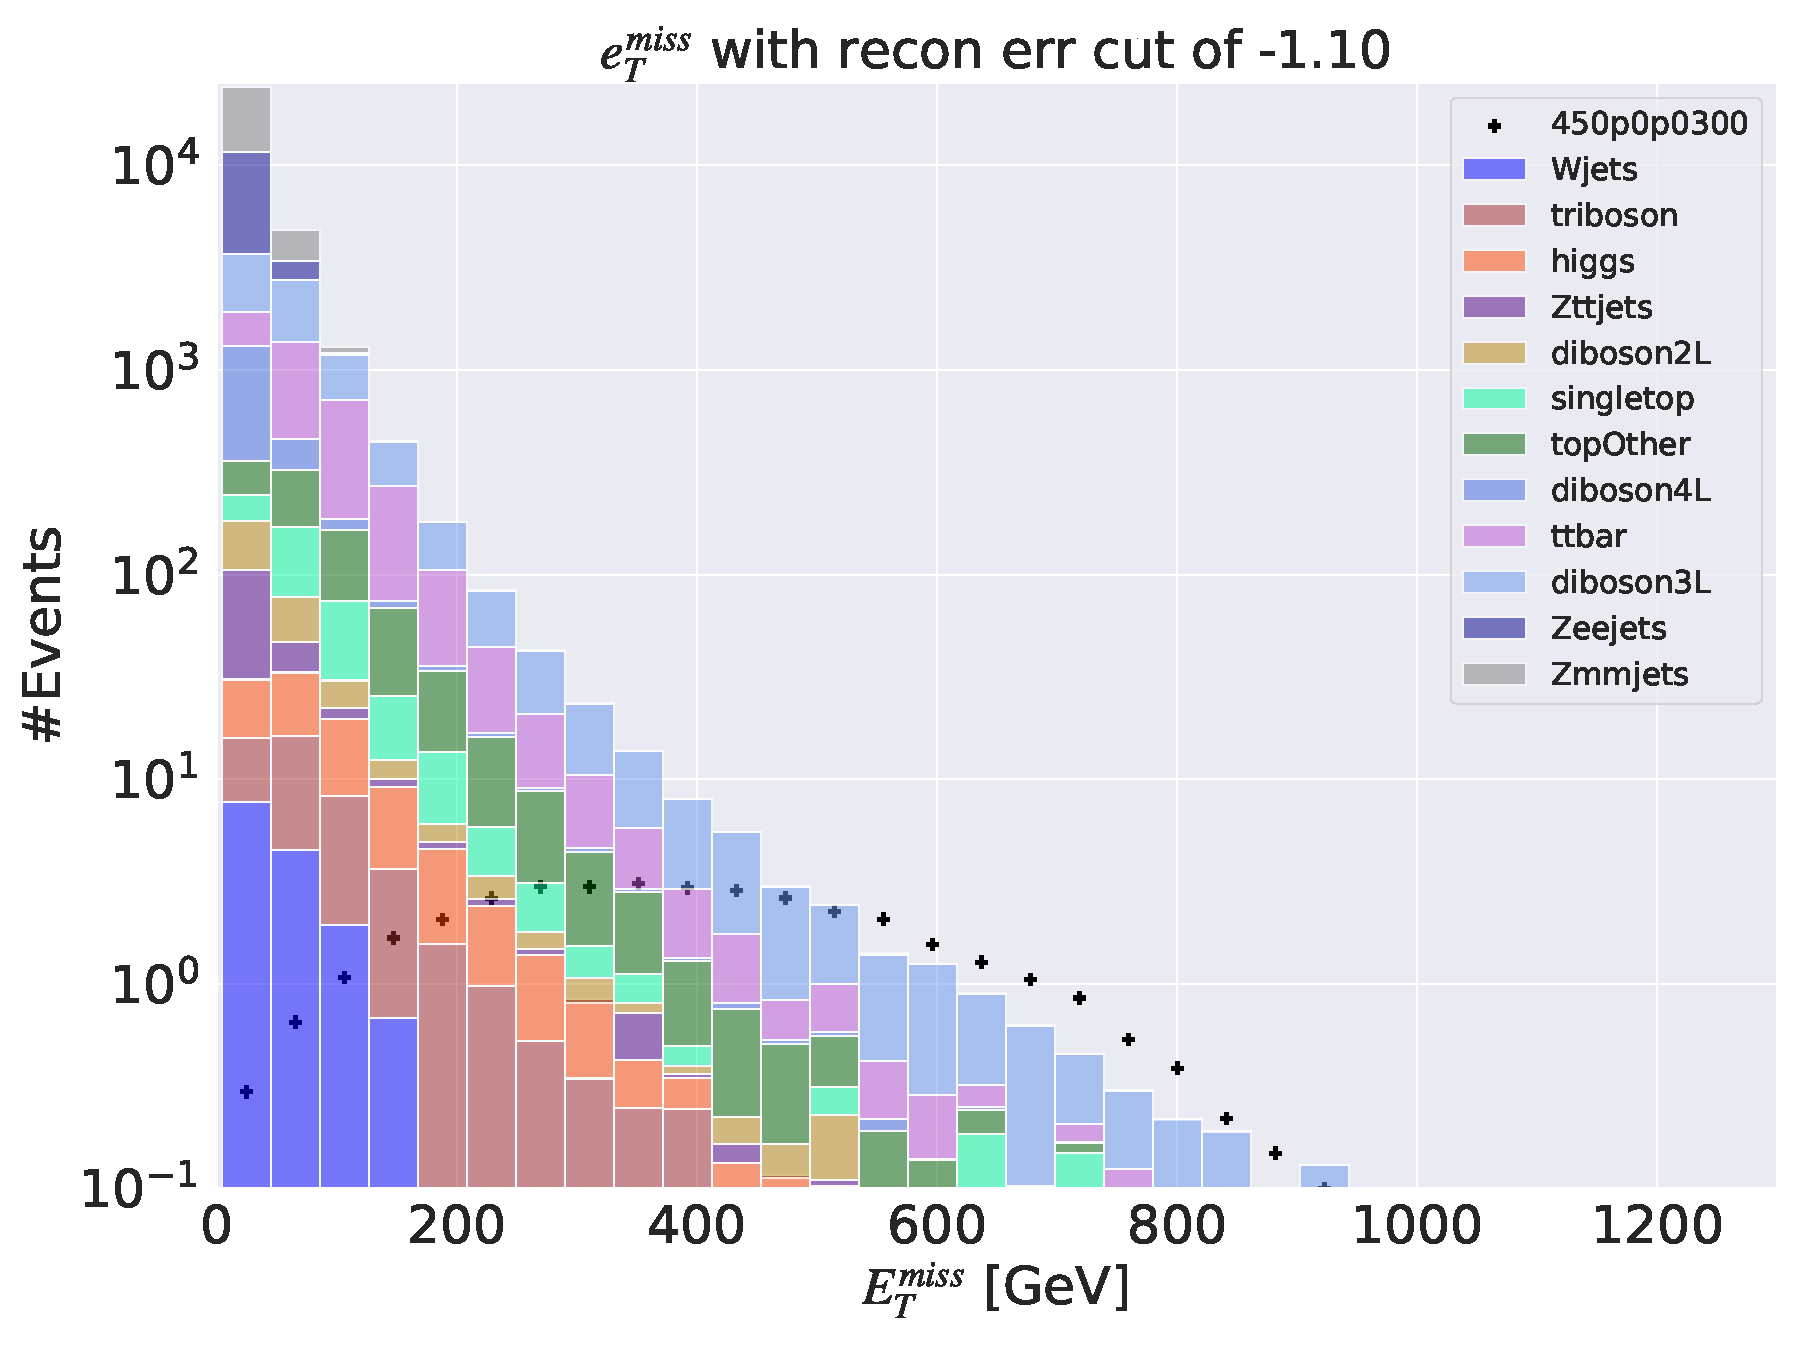
\includegraphics[width=\textwidth]{Figures/VAE_testing/big/3lep/b_data_recon_big_rm3_feats_sig_450p0p0300_etmiss_recon_errcut_-1.10.pdf}
        \caption{}
        \label{fig:VAE_3lep_big_etmiss_450}
    \end{subfigure}
    \hfill
    \begin{subfigure}{.49\textwidth}
        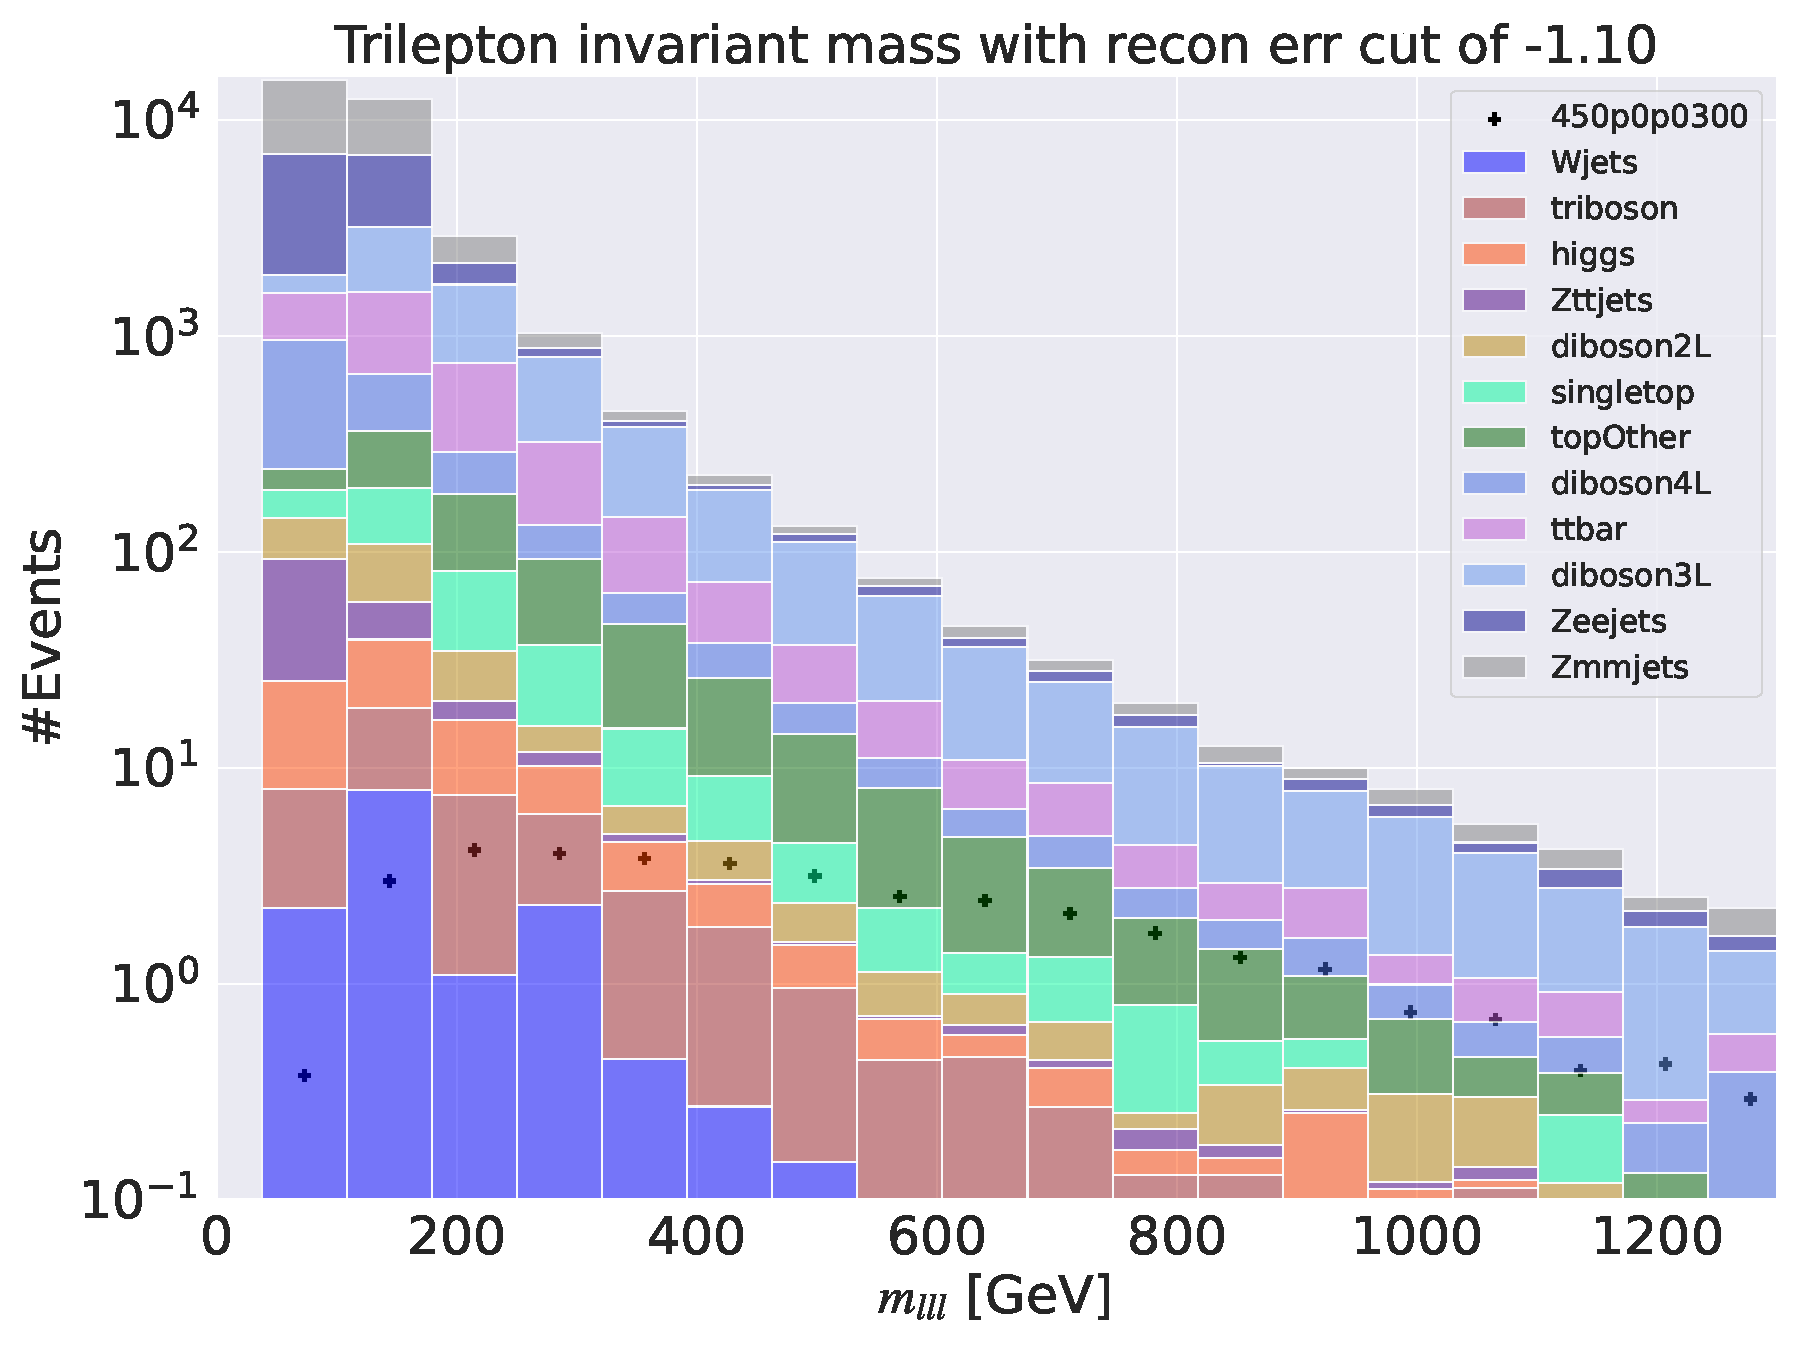
\includegraphics[width=\textwidth]{Figures/VAE_testing/big/3lep/b_data_recon_big_rm3_feats_sig_450p0p0300_mlll_recon_errcut_-1.10.pdf}
        \caption{}
        \label{fig:VAE_3lep_big_mlll_450}
    \end{subfigure}
    \hfill   
    \begin{subfigure}{.49\textwidth}
        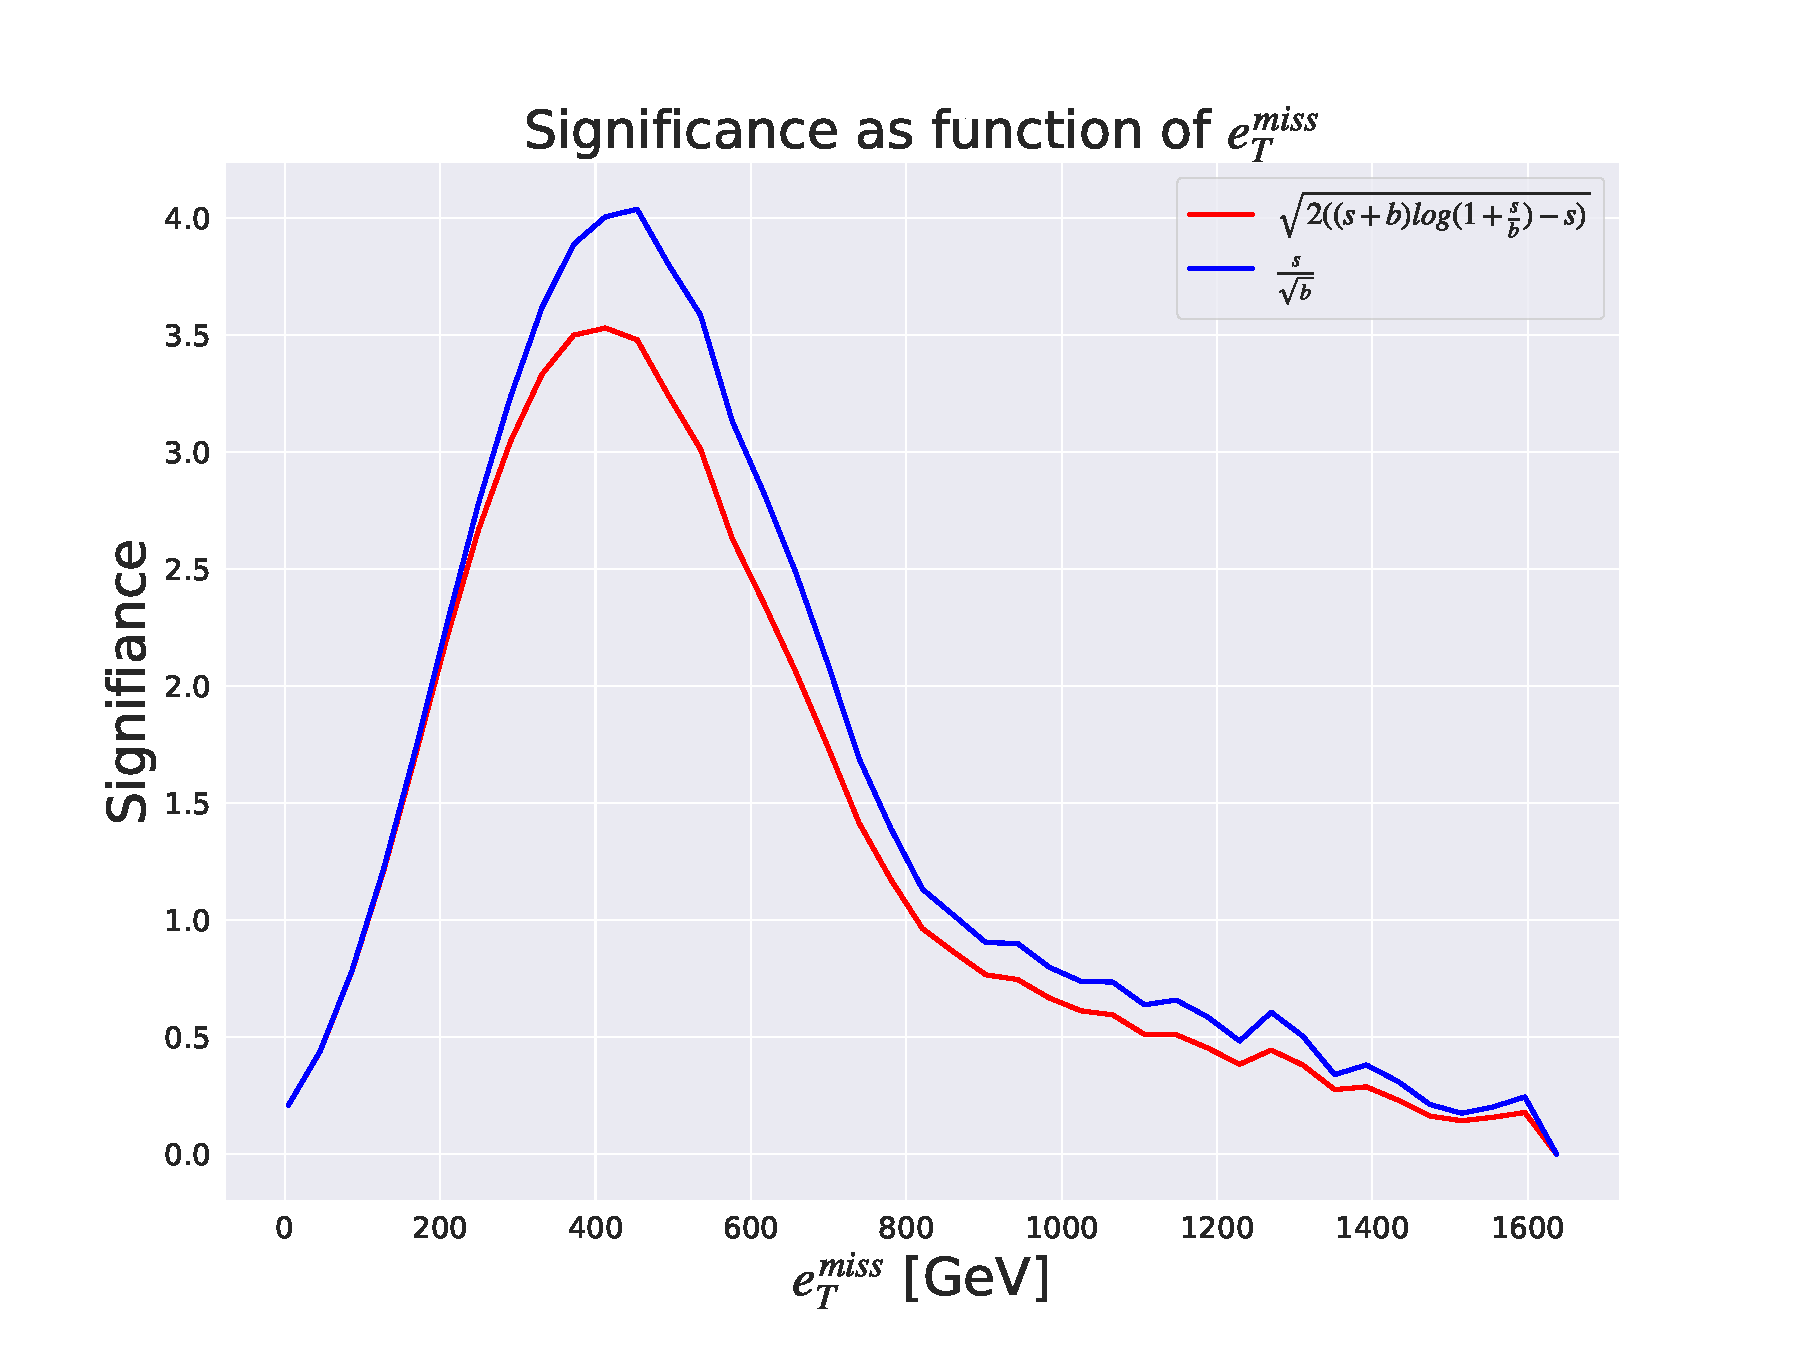
\includegraphics[width=\textwidth]{Figures/VAE_testing/big/3lep/significance_etmiss_450p0p0300_-1.0969148715571329.pdf}
        \caption{}
        \label{fig:VAE_3lep_big_signi_450}
    \end{subfigure}
    \hfill      
    \caption[3lep deep network | $450p300$ | VAE]{Reconstruction error, $e_T^{miss}$ signal region, $m_{lll}$ signal region and significance as function of 
    $e_T^{miss}$ for the deep variational autoencoder using the SUSY $450p300$.
    Figure \ref{fig:VAE_3lep_big_450} shows the reconstruction error 
    distribution for the SM MC and the SUSY signal. Here the autoencoder produces a hill-like for background and 
    signal with little destinction. The peaks of the two distributions are not separated in reconstruction error. Figure \ref{fig:VAE_3lep_big_etmiss_450} 
    shows the $e_T^{miss}$ distribution for the SM MC and the SUSY signal in the signal region, defined as the region having a $log_{10}$ 
    reconstruction error above -1.10. Some background is removed, and the peaks of the SM MC and signal 
    distributions are separated. Figure \ref{fig:VAE_3lep_big_mlll_450} shows the $m_{lll}$ distribution for the SM MC and the SUSY signal. 
    The shape of the SM MC and the signal distributions are displaying almost the same shape. Figure \ref{fig:VAE_3lep_big_signi_450} shows the significance as 
    function of $e_T^{miss}$. The maximum significance is found when applying a cut of about > 450 GeV in the $e_T^{miss}$, with a significance of around $4.1$.}
    \label{fig:VAE_3lep_big_rec_sig_signi_450}
\end{figure}

\begin{figure}[!htb]
    \centering
    \begin{subfigure}{.49\textwidth}
        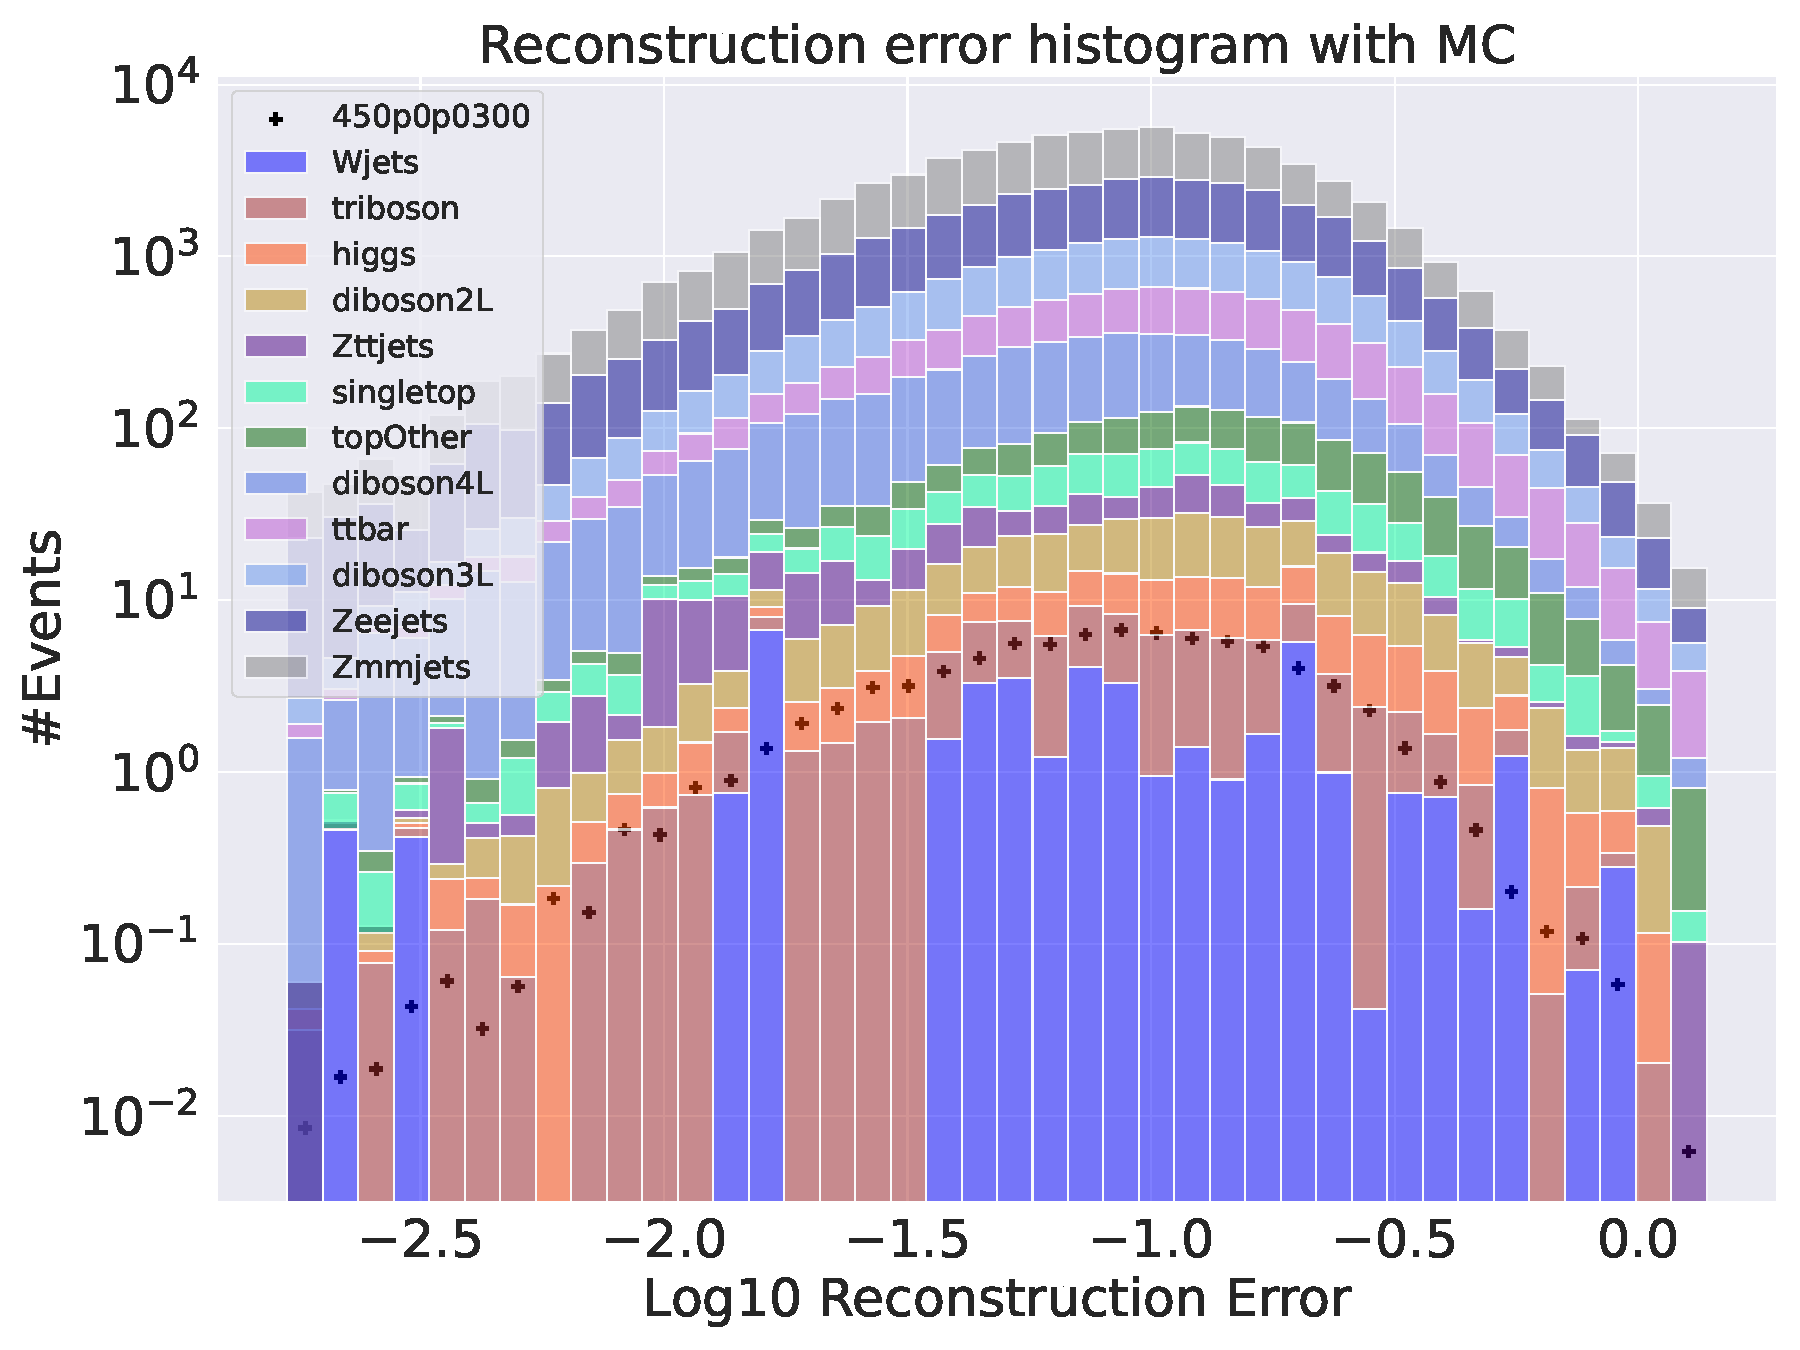
\includegraphics[width=\textwidth]{Figures/VAE_testing/small/3lep/b_data_recon_big_rm3_feats_sig_450p0p0300.pdf}
        \caption{ }
        \label{fig:VAE_3lep_small_450}
    \end{subfigure}
    \hfill
    \begin{subfigure}{.49\textwidth}
        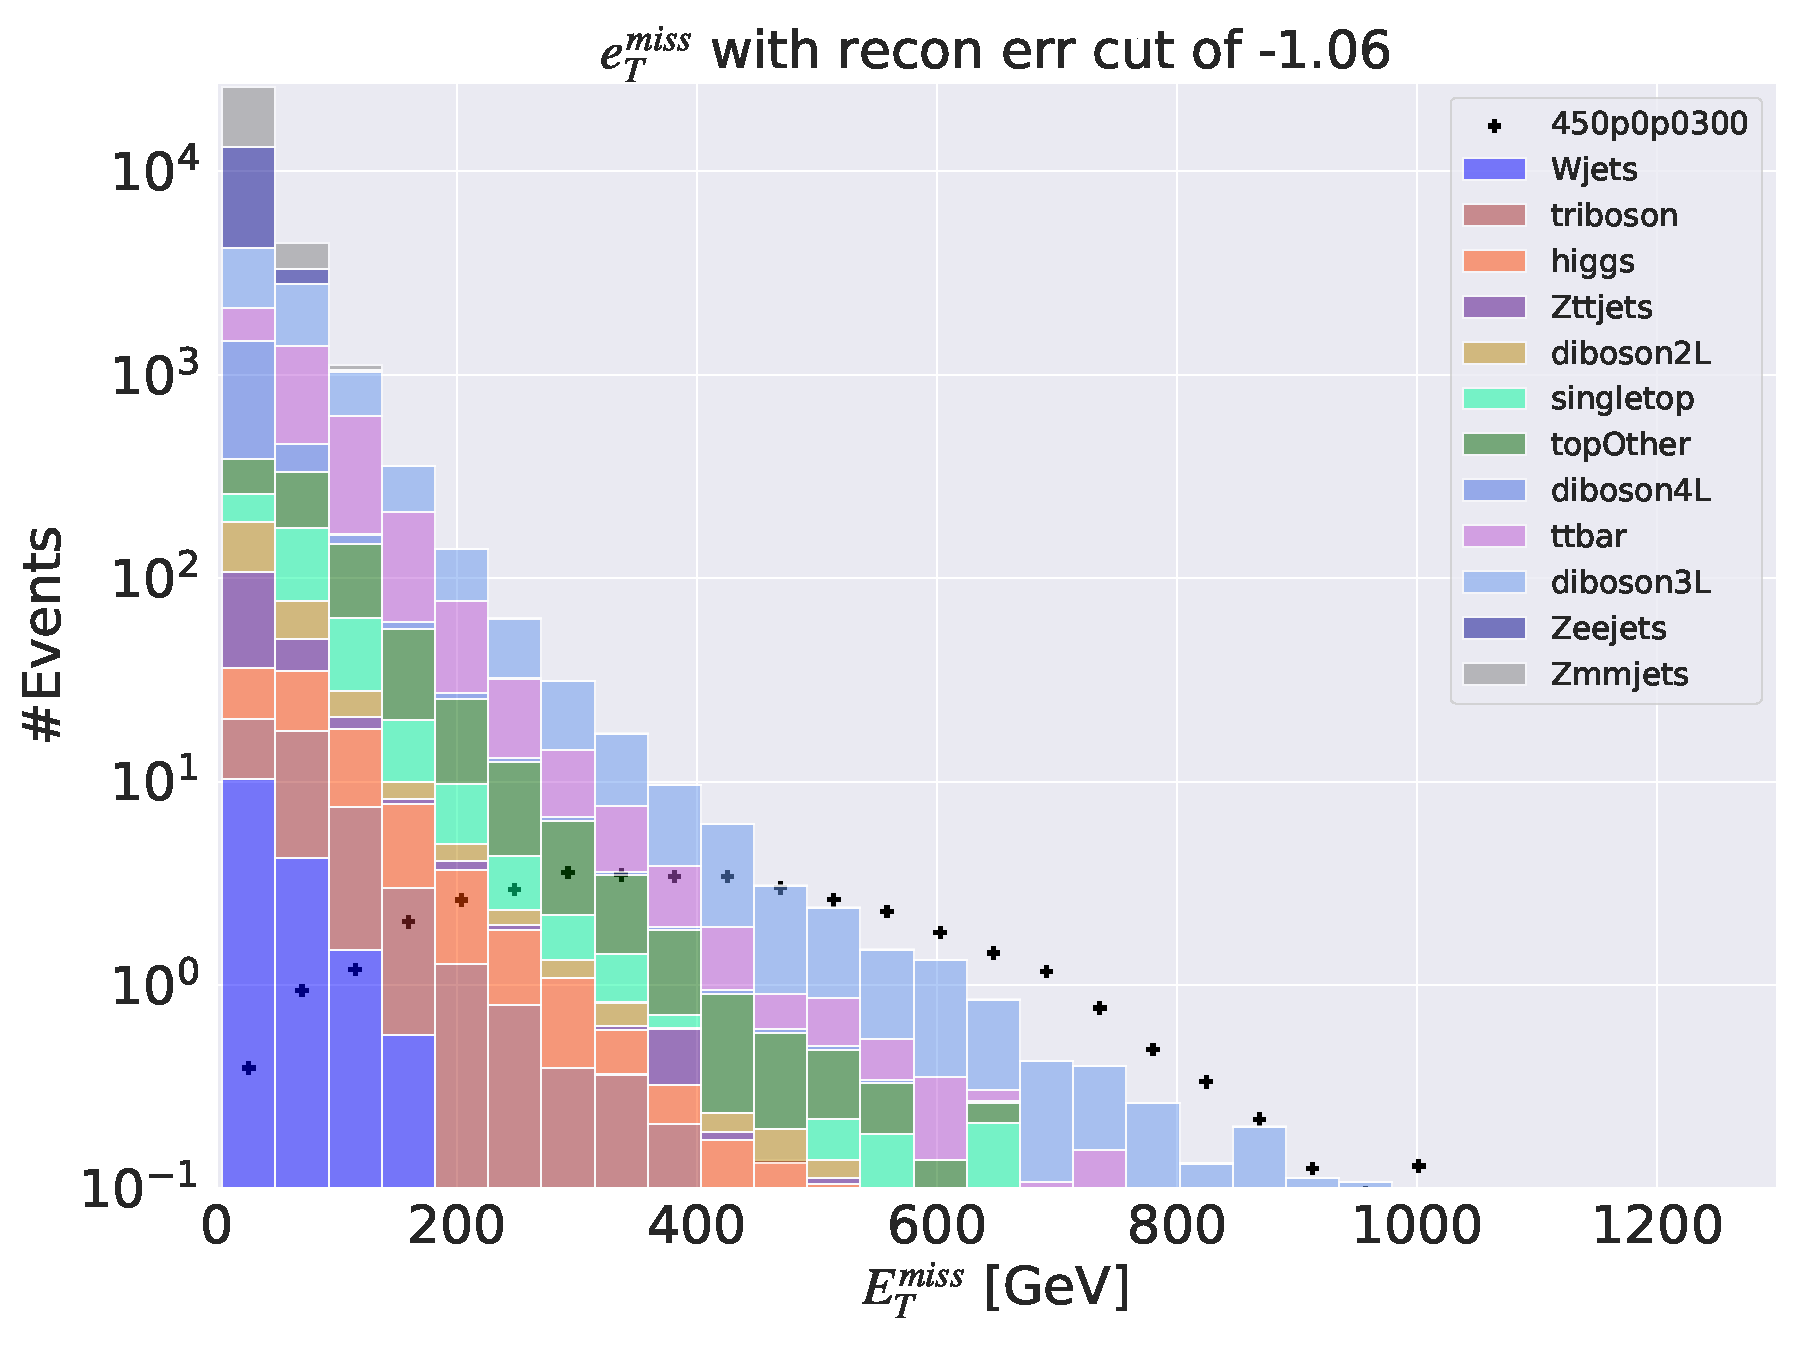
\includegraphics[width=\textwidth]{Figures/VAE_testing/small/3lep/b_data_recon_big_rm3_feats_sig_450p0p0300_etmiss_recon_errcut_-1.06.pdf}
        \caption{}
        \label{fig:VAE_3lep_small_etmiss_450}
    \end{subfigure}
    \hfill
    \begin{subfigure}{.49\textwidth}
        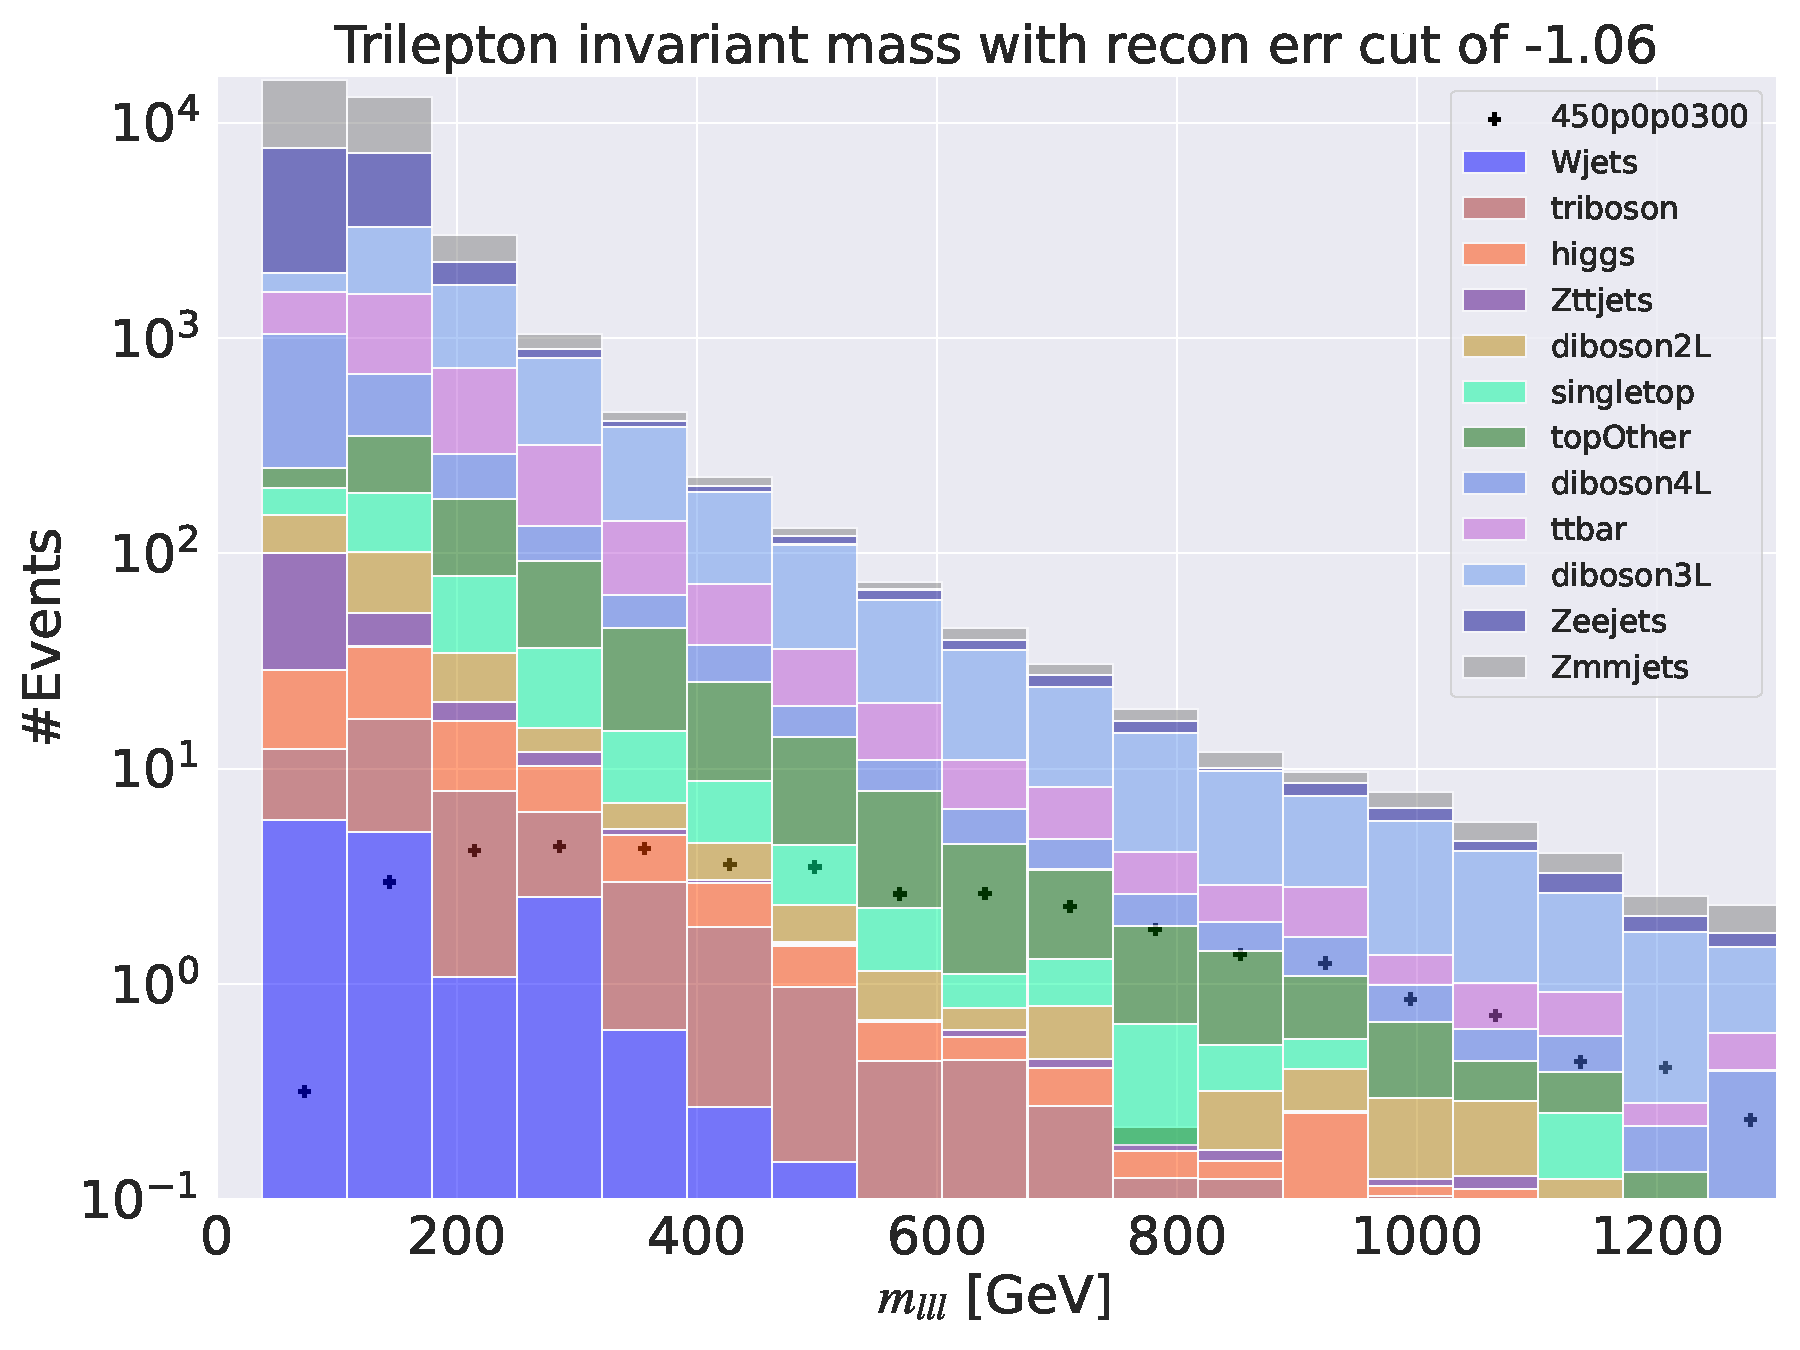
\includegraphics[width=\textwidth]{Figures/VAE_testing/small/3lep/b_data_recon_big_rm3_feats_sig_450p0p0300_mlll_recon_errcut_-1.06.pdf}
        \caption{}
        \label{fig:VAE_3lep_small_mlll_450}
    \end{subfigure}
    \hfill   
    \begin{subfigure}{.49\textwidth}
        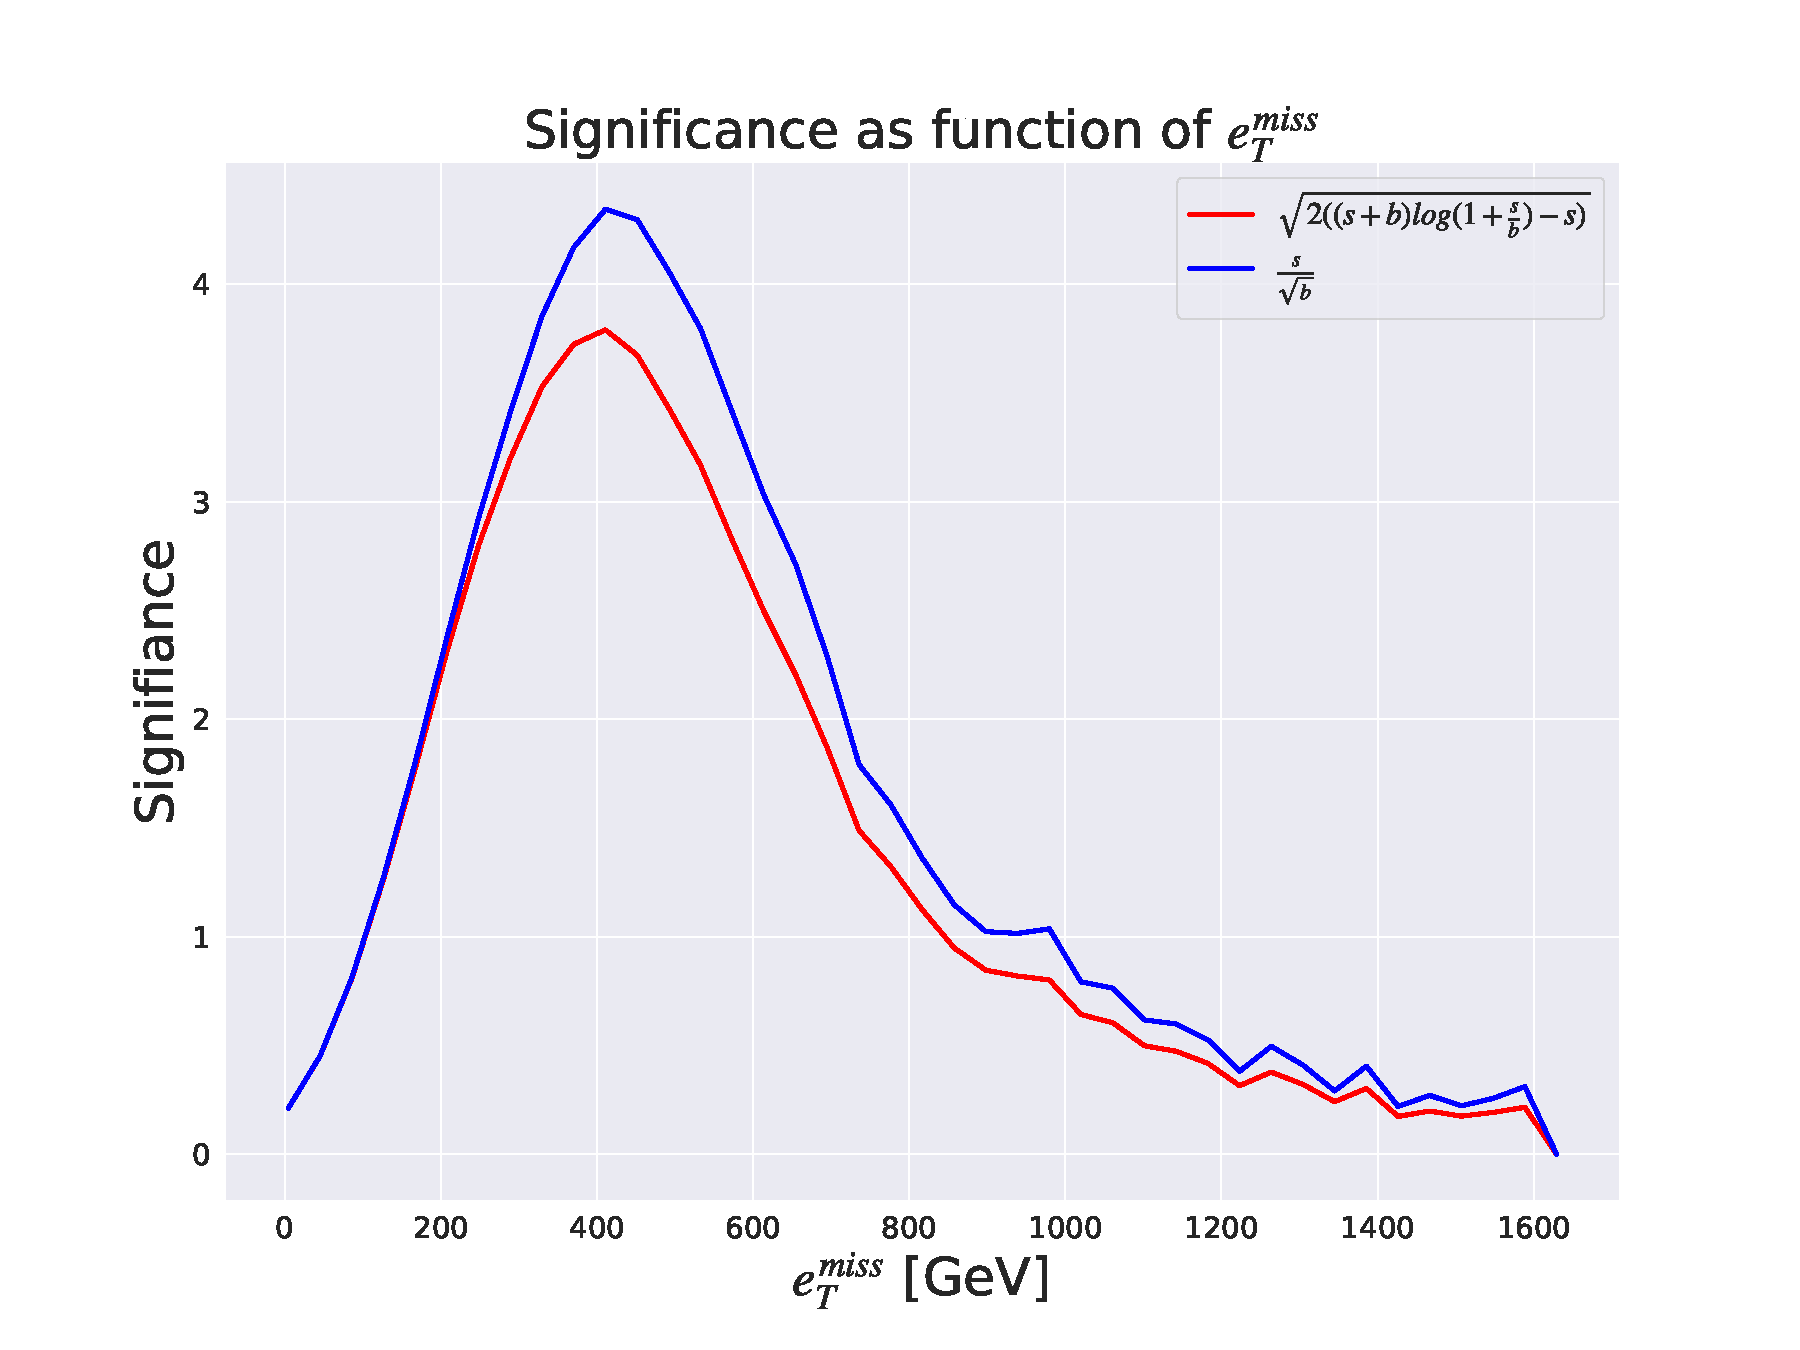
\includegraphics[width=\textwidth]{Figures/VAE_testing/small/3lep/significance_etmiss_450p0p0300_-1.0610372272331543.pdf}
        \caption{}
        \label{fig:VAE_3lep_small_signi_450}
    \end{subfigure}
    \hfill      
    \caption[3lep shallow network | $450p300$ | VAE]{Reconstruction error, $e_T^{miss}$ signal region, $m_{lll}$ signal region and significance as function of 
    $e_T^{miss}$ for the shallow variational autoencoder using the SUSY $450p300$. 
    Figure \ref{fig:VAE_3lep_small_450} shows the reconstruction error 
    distribution for the SM MC and the SUSY signal. Here the autoencoder produces a hill-like for background and 
    signal with little destinction. The peaks of the two distributions are not separated in reconstruction error. Figure \ref{fig:VAE_3lep_small_etmiss_450} 
    shows the $e_T^{miss}$ distribution for the SM MC and the SUSY signal in the signal region, defined as the region having a $log_{10}$ 
    reconstruction error above -1.06. Some background is removed, and the peaks of the SM MC and signal 
    distributions are separated. Figure \ref{fig:VAE_3lep_small_mlll_450} shows the $m_{lll}$ distribution for the SM MC and the SUSY signal. 
    The shape of the SM MC and the signal distributions are displaying almost the same shape. Figure \ref{fig:VAE_3lep_small_signi_450} shows the significance as 
    function of $e_T^{miss}$. The maximum significance is found when applying a cut of about > 400 GeV in the $e_T^{miss}$, with a significance of around $4.5$.}
    \label{fig:VAE_3lep_small_rec_sig_signi_450}
\end{figure}








\begin{figure}[!htb]
    \centering
    \begin{subfigure}{.49\textwidth}
        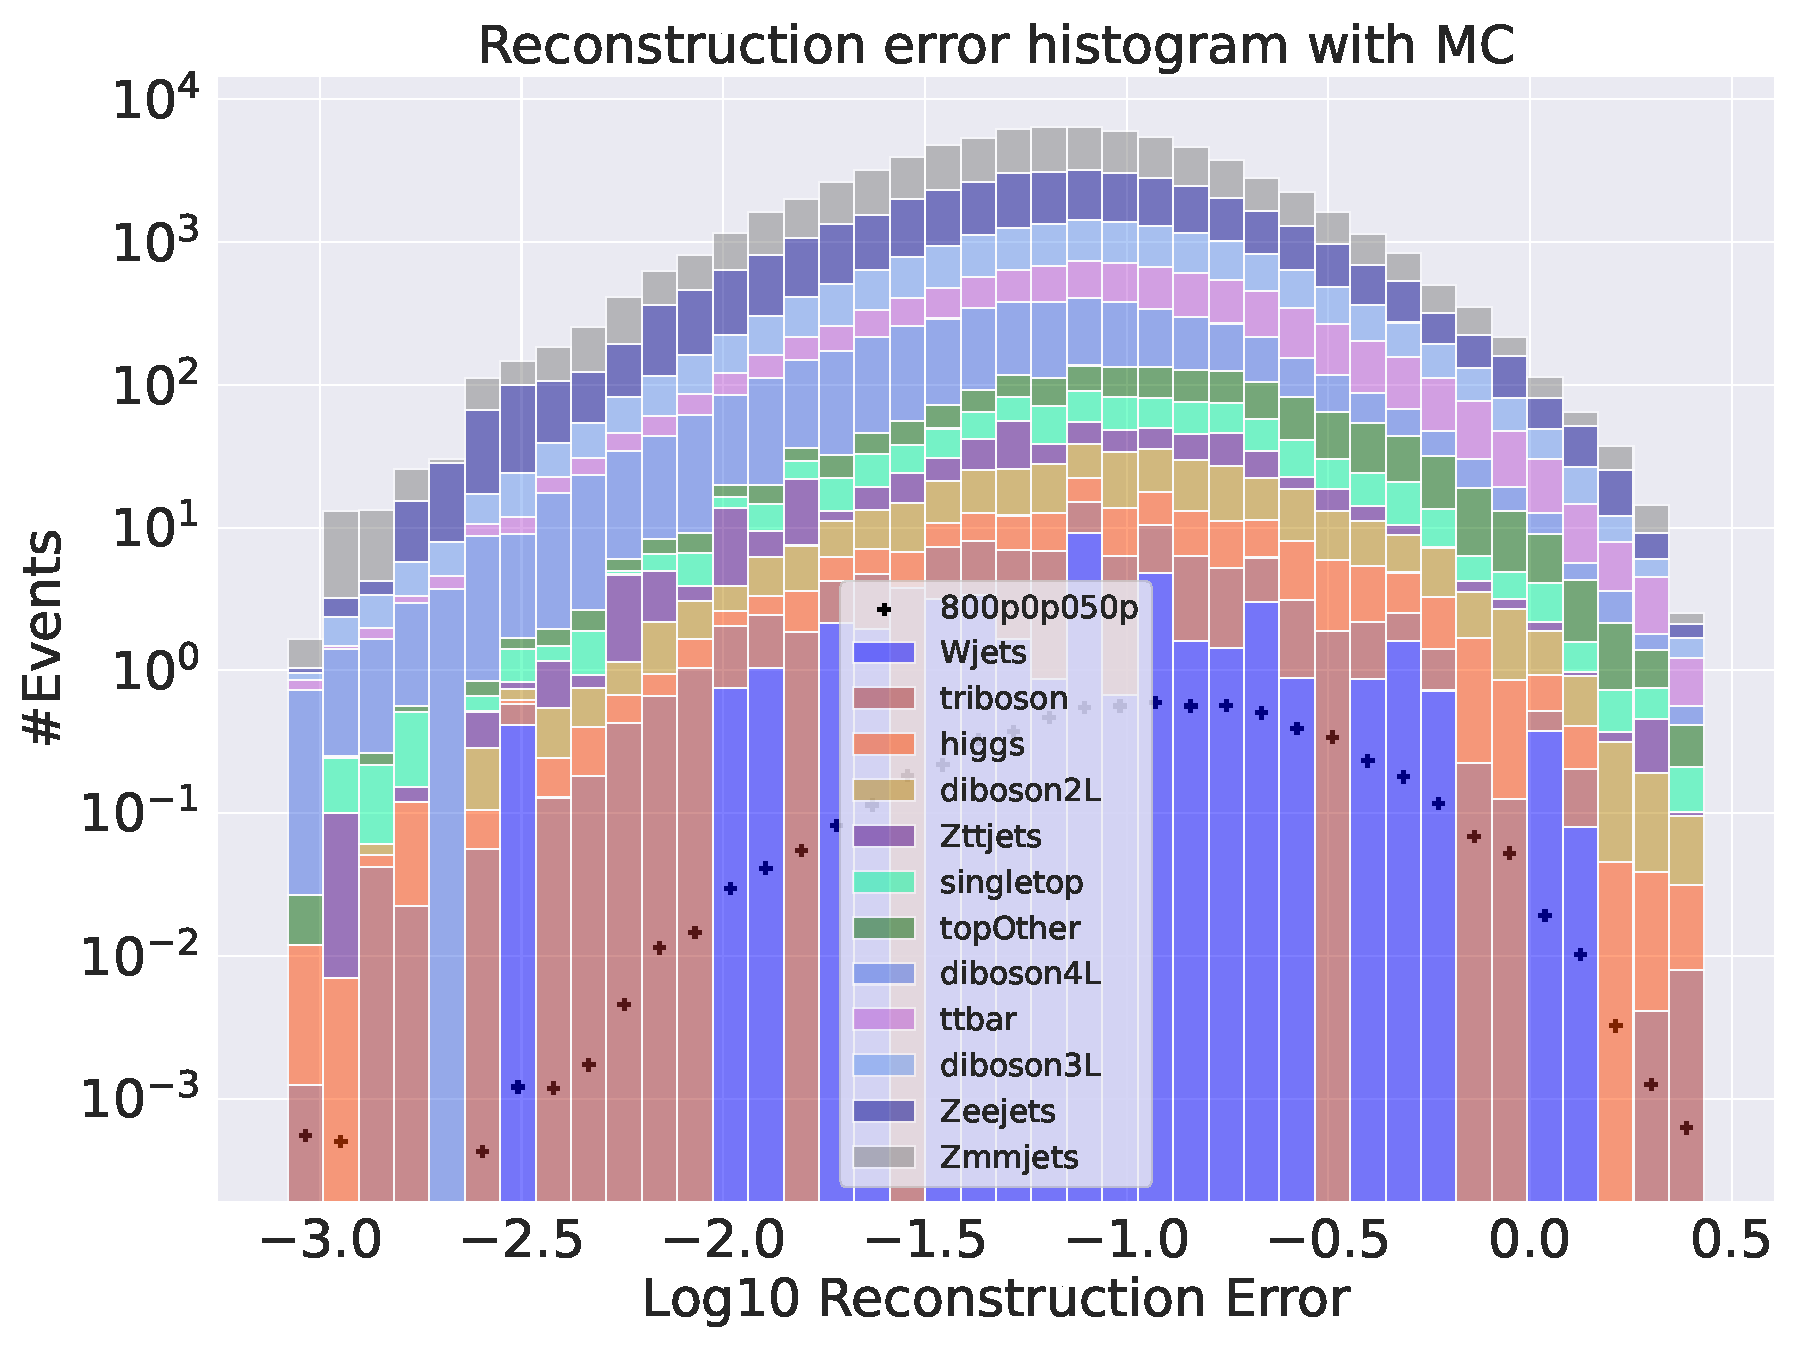
\includegraphics[width=\textwidth]{Figures/VAE_testing/big/3lep/b_data_recon_big_rm3_feats_sig_800p0p050p.pdf}
        \caption{ }
        \label{fig:VAE_3lep_big_800}
    \end{subfigure}
    \hfill
    \begin{subfigure}{.49\textwidth}
        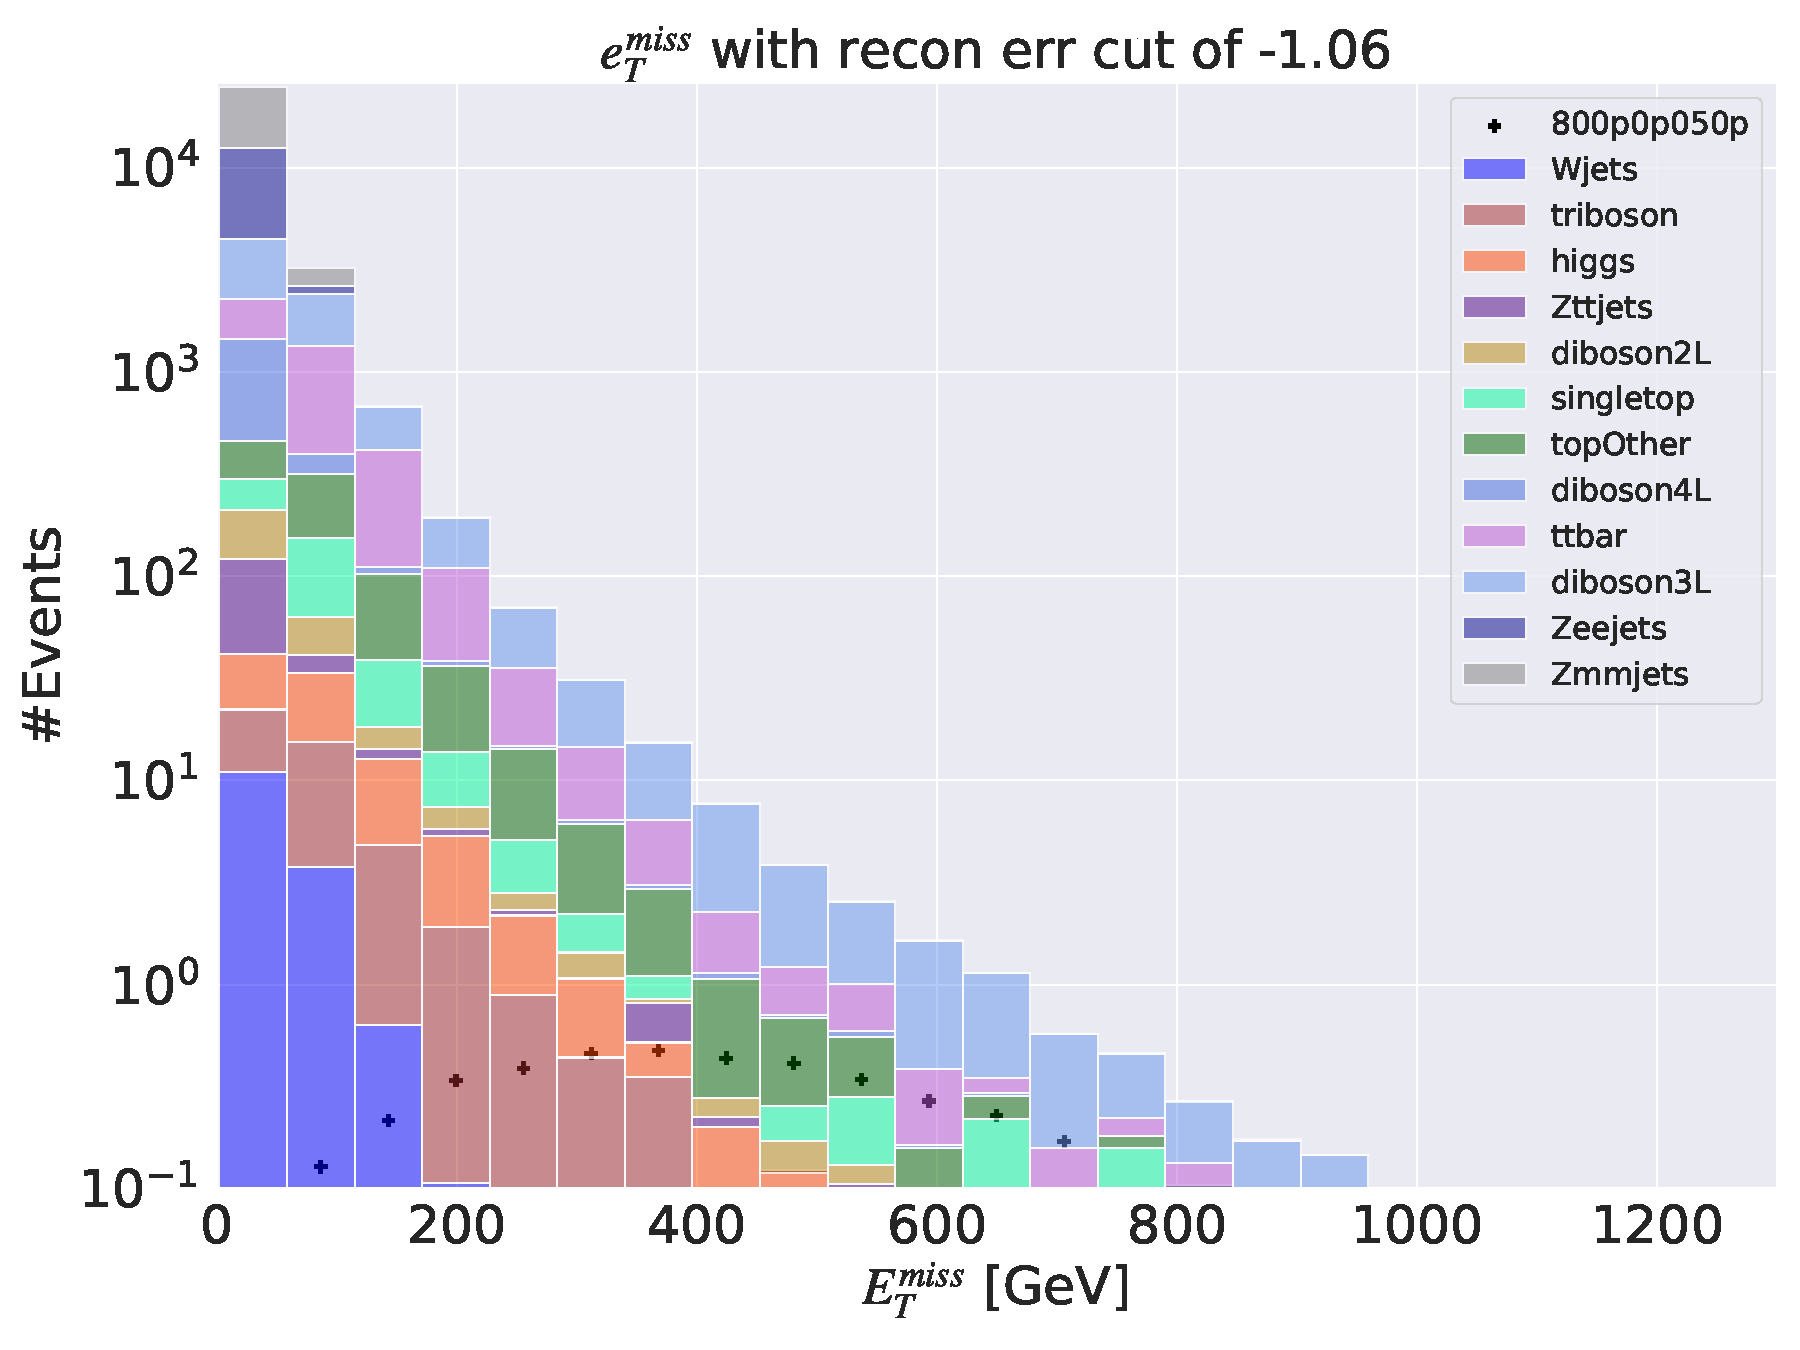
\includegraphics[width=\textwidth]{Figures/VAE_testing/big/3lep/b_data_recon_big_rm3_feats_sig_800p0p050p_etmiss_recon_errcut_-1.06.pdf}
        \caption{}
        \label{fig:VAE_3lep_big_etmiss_800}
    \end{subfigure}
    \hfill
    \begin{subfigure}{.49\textwidth}
        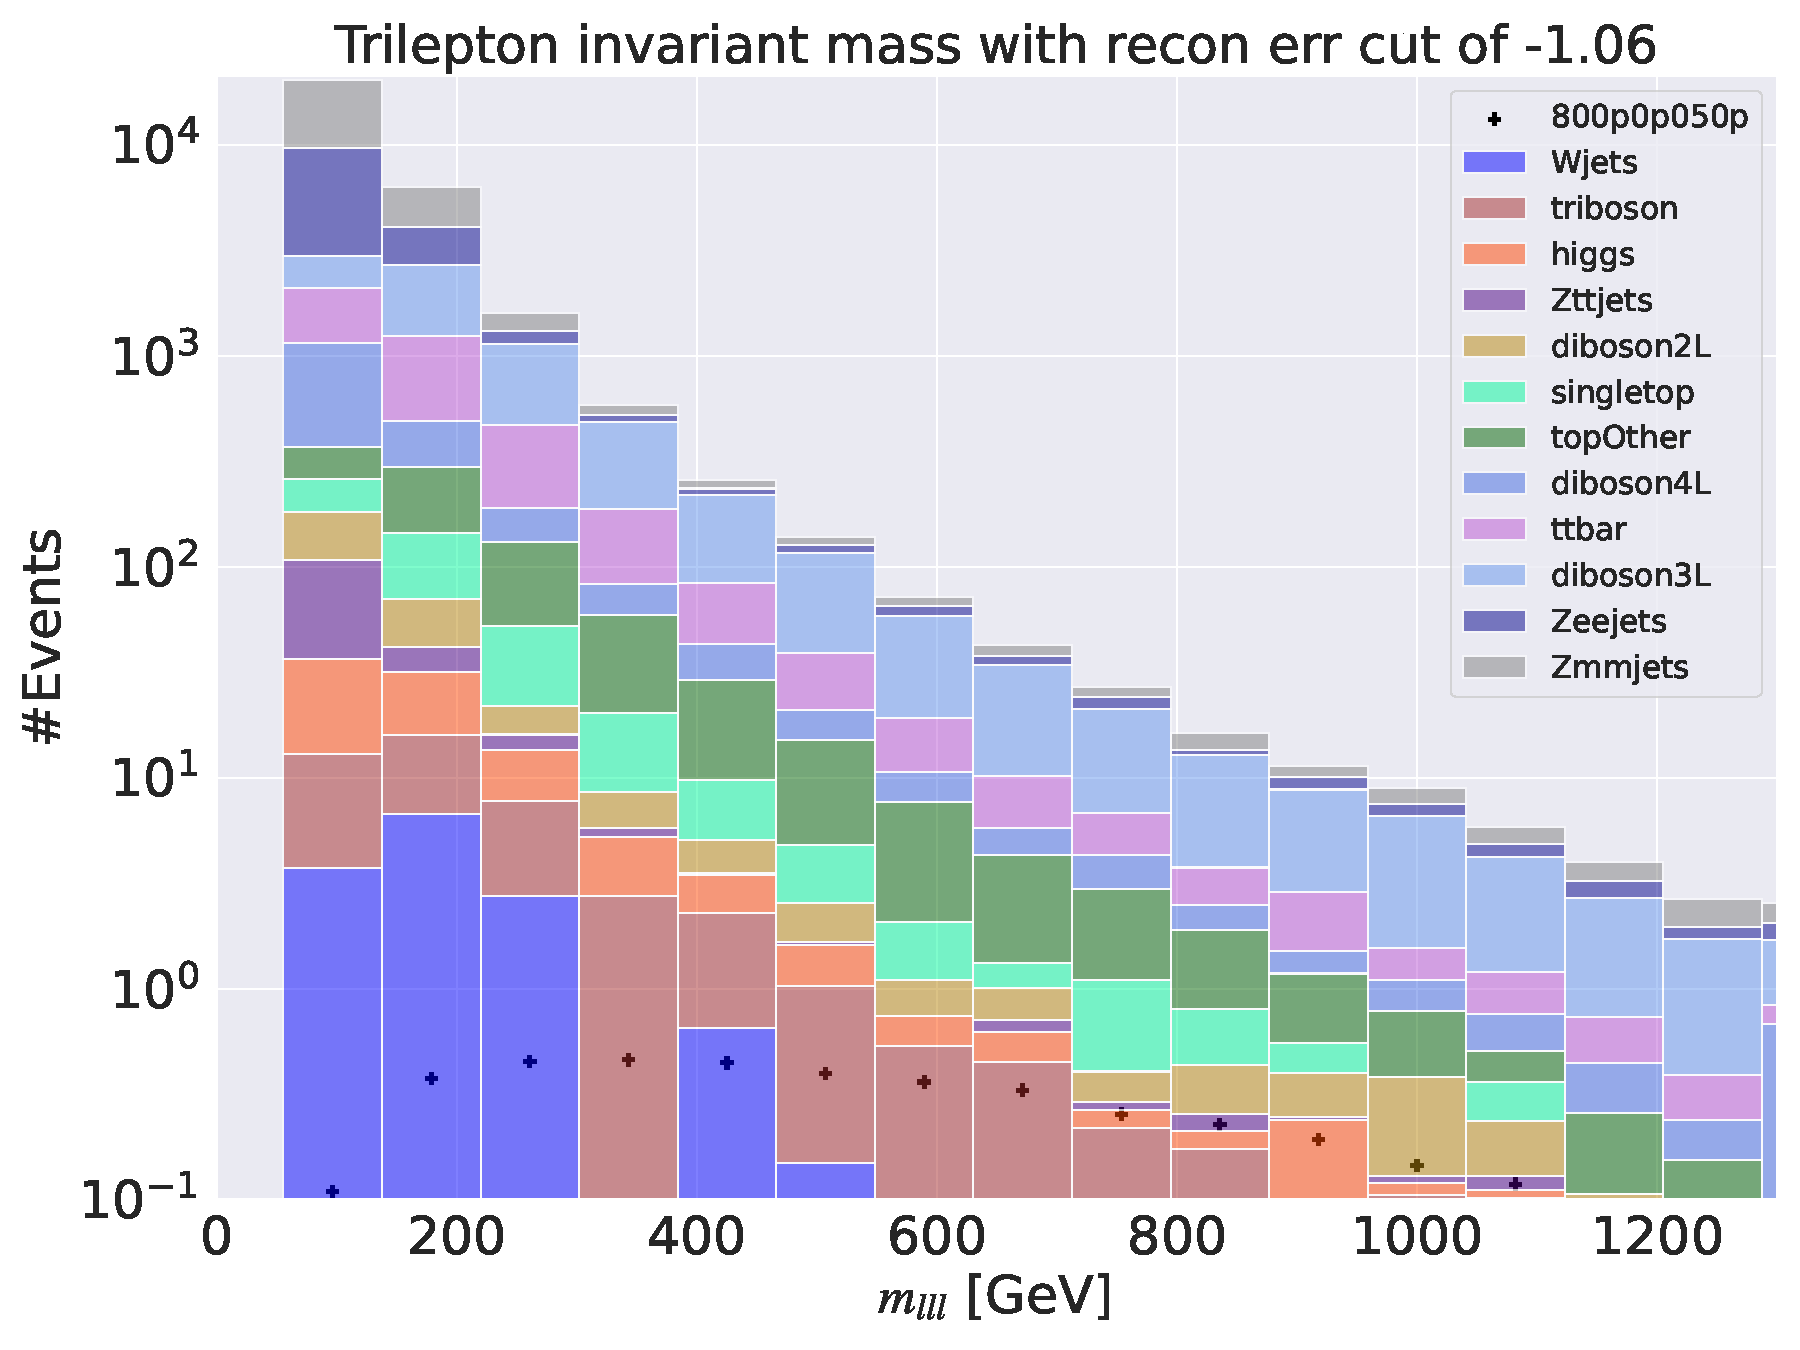
\includegraphics[width=\textwidth]{Figures/VAE_testing/big/3lep/b_data_recon_big_rm3_feats_sig_800p0p050p_mlll_recon_errcut_-1.06.pdf}
        \caption{}
        \label{fig:VAE_3lep_big_mlll_800}
    \end{subfigure}
    \hfill   
    \begin{subfigure}{.49\textwidth}
        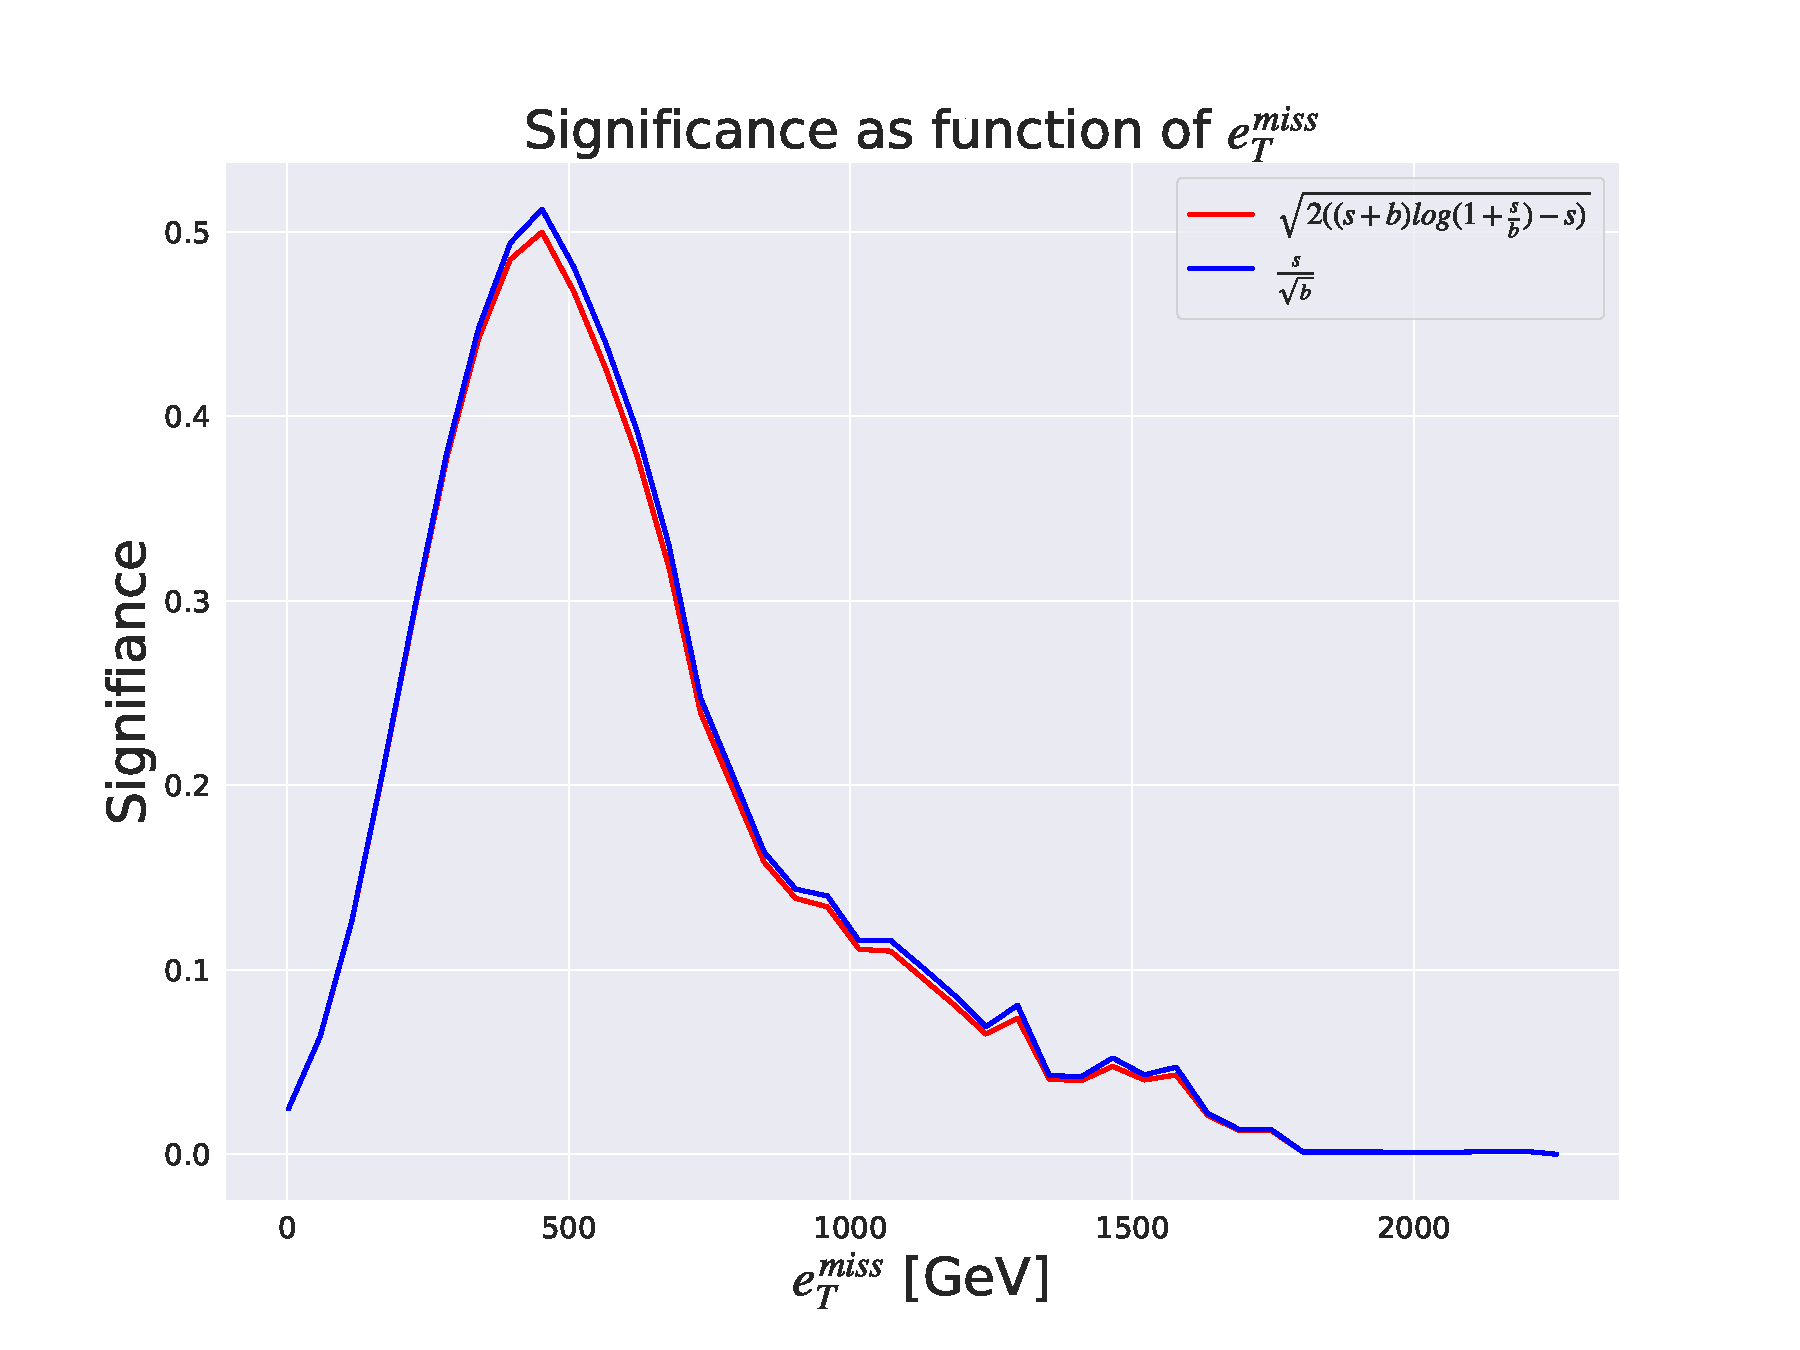
\includegraphics[width=\textwidth]{Figures/VAE_testing/big/3lep/significance_etmiss_800p0p050p_-1.0588523538160817.pdf}
        \caption{}
        \label{fig:VAE_3lep_big_signi_800}
    \end{subfigure}
    \hfill      
    \caption[3lep deep network | $800p50$ | VAE]{Reconstruction error, $e_T^{miss}$ signal region, $m_{lll}$ signal region and significance as function of 
    $e_T^{miss}$ for the deep variational autoencoder using the SUSY $800p50$.
    Figure \ref{fig:VAE_3lep_big_800} shows the reconstruction error 
    distribution for the SM MC and the SUSY signal. Here the autoencoder produces a hill-like for background and 
    signal with little destinction. The peaks of the two distributions are not separated in reconstruction error. Figure \ref{fig:VAE_3lep_big_etmiss_800} 
    shows the $e_T^{miss}$ distribution for the SM MC and the SUSY signal in the signal region, defined as the region having a $log_{10}$ 
    reconstruction error above -1.06. Some background is removed, and the peaks of the SM MC and signal 
    distributions are separated. Figure \ref{fig:VAE_3lep_big_mlll_800} shows the $m_{lll}$ distribution for the SM MC and the SUSY signal. 
    The shape of the SM MC and the signal distributions are displaying almost the same shape. Figure \ref{fig:VAE_3lep_big_signi_800} shows the significance as 
    function of $e_T^{miss}$. The maximum significance is found when applying a cut of about > 480 GeV in the $e_T^{miss}$, with a significance of around $0.6$.}
    \label{fig:VAE_3lep_big_rec_sig_signi_800}
\end{figure}

\begin{figure}[!htb]
    \centering
    \begin{subfigure}{.49\textwidth}
        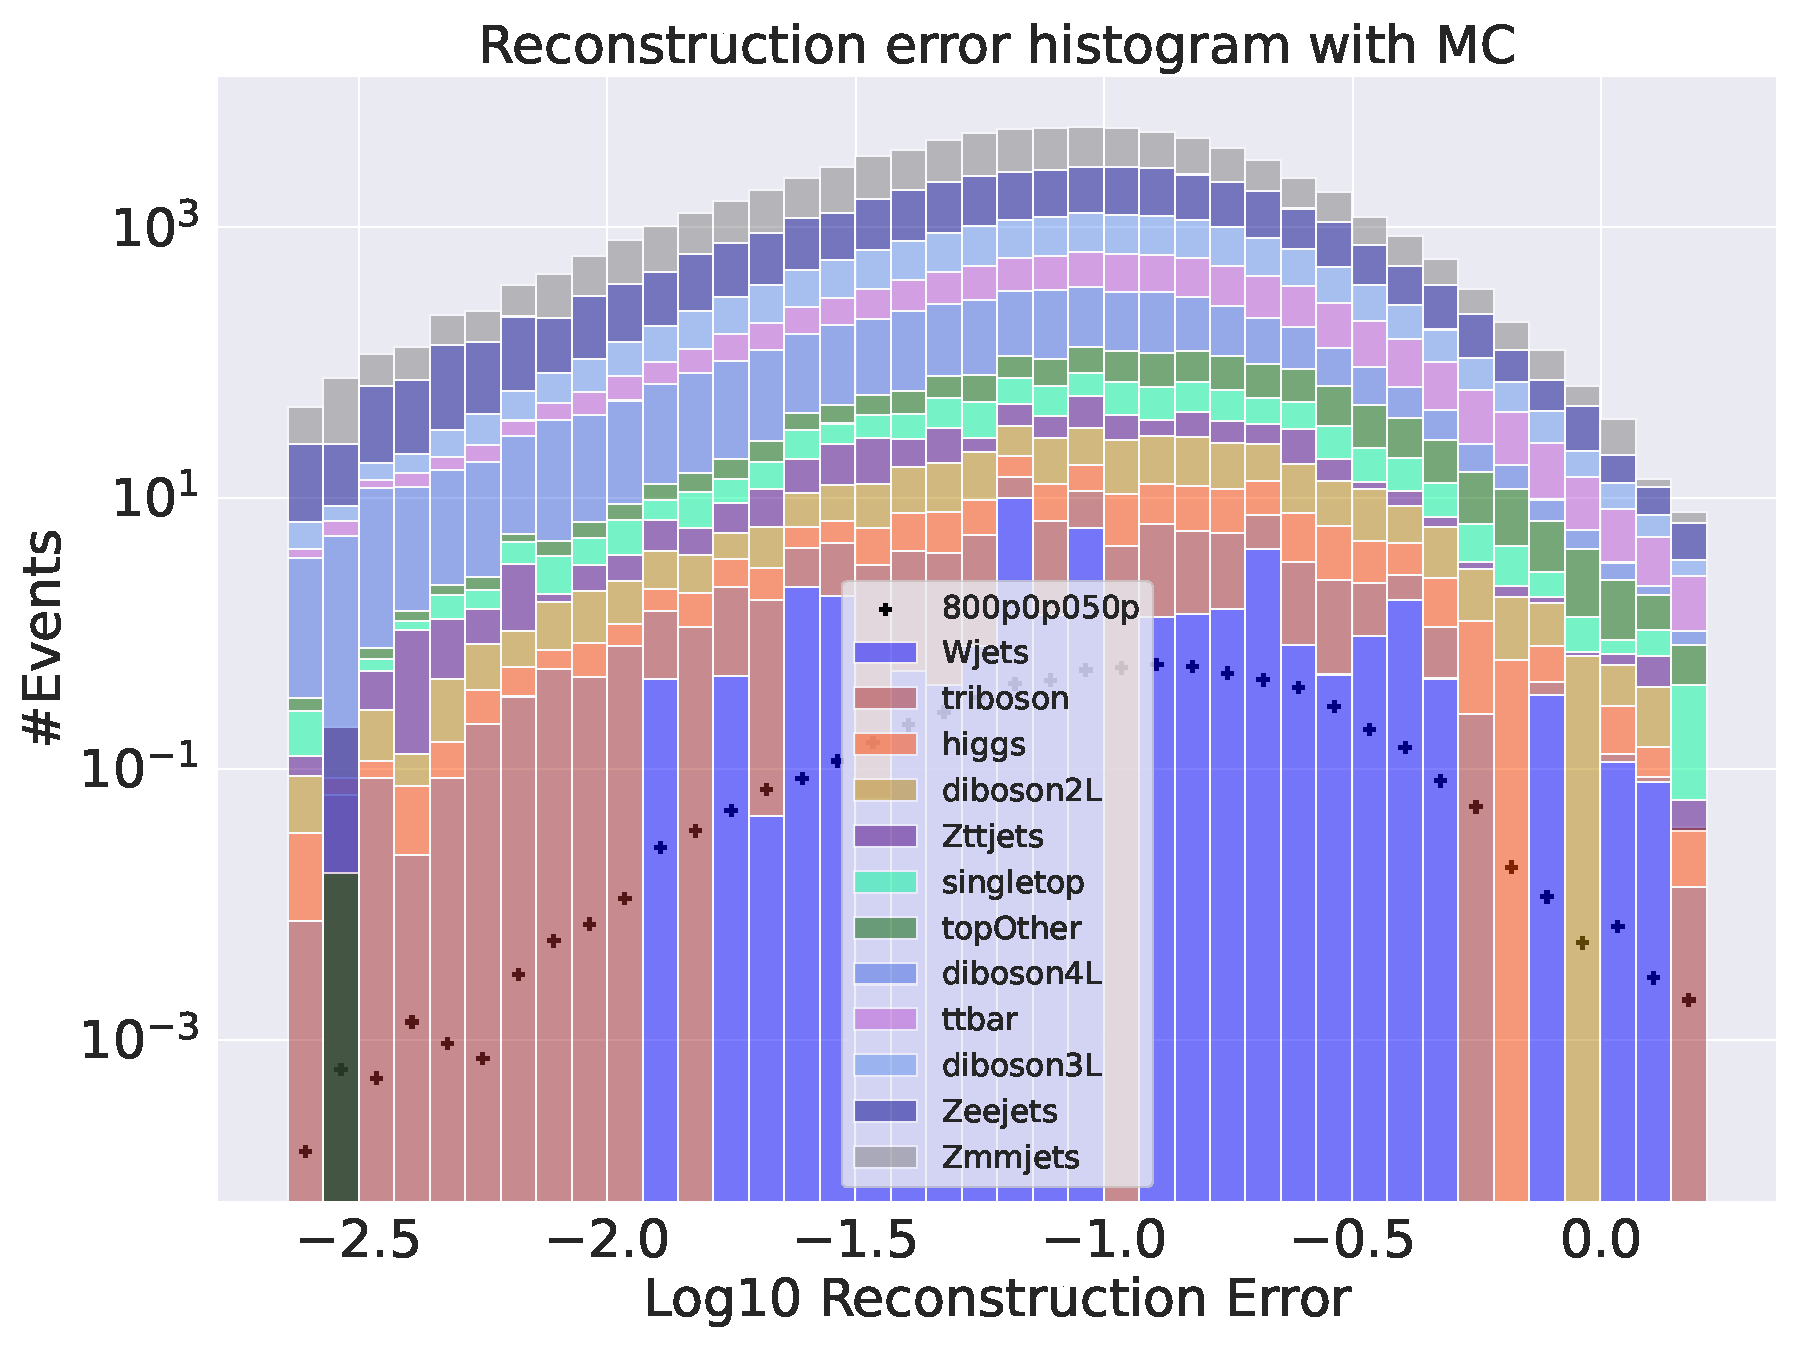
\includegraphics[width=\textwidth]{Figures/VAE_testing/small/3lep/b_data_recon_big_rm3_feats_sig_800p0p050p.pdf}
        \caption{ }
        \label{fig:VAE_3lep_small_800}
    \end{subfigure}
    \hfill
    \begin{subfigure}{.49\textwidth}
        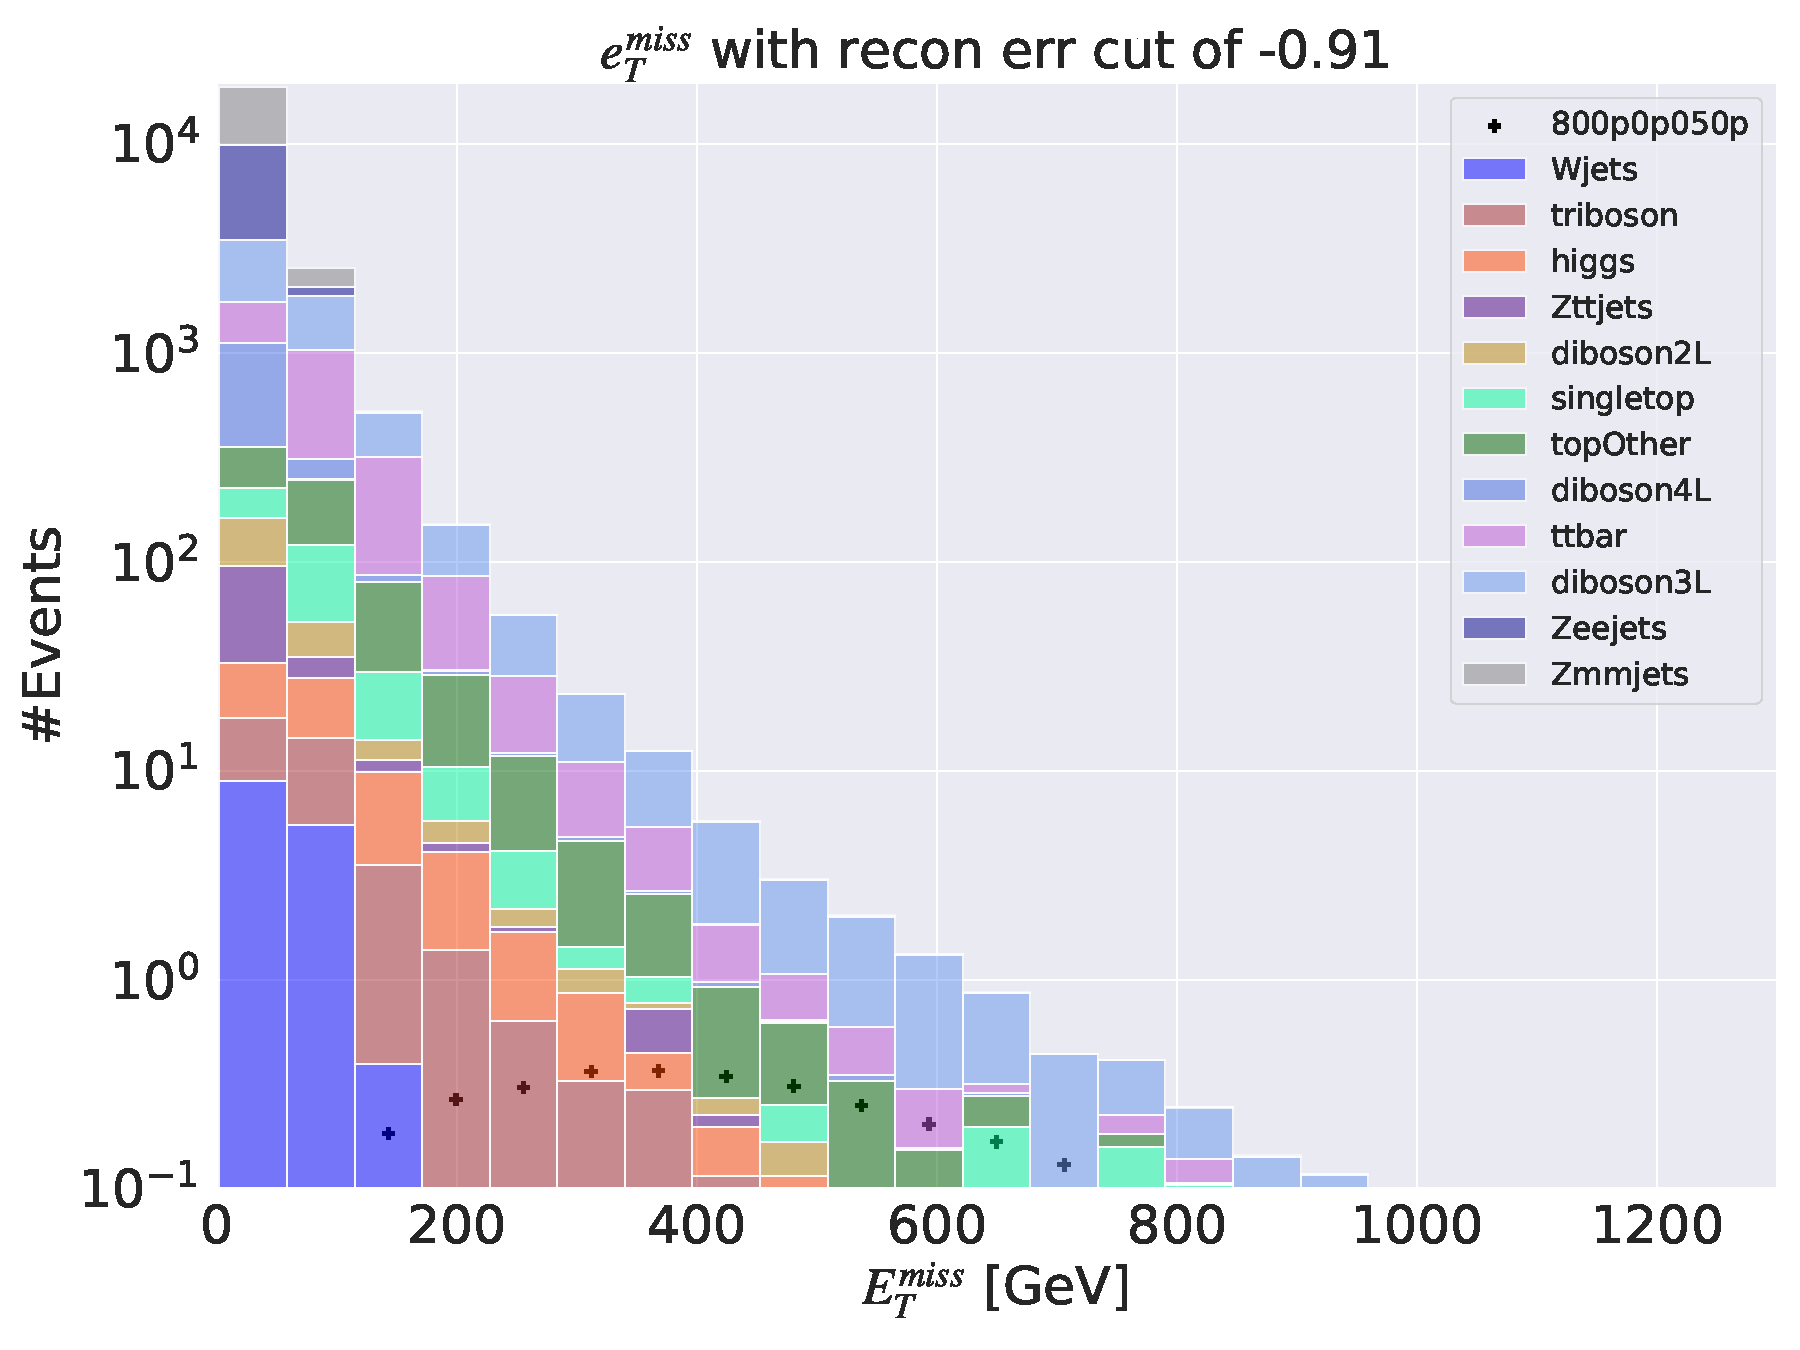
\includegraphics[width=\textwidth]{Figures/VAE_testing/small/3lep/b_data_recon_big_rm3_feats_sig_800p0p050p_etmiss_recon_errcut_-0.91.pdf}
        \caption{}
        \label{fig:VAE_3lep_small_etmiss_800}
    \end{subfigure}
    \hfill
    \begin{subfigure}{.49\textwidth}
        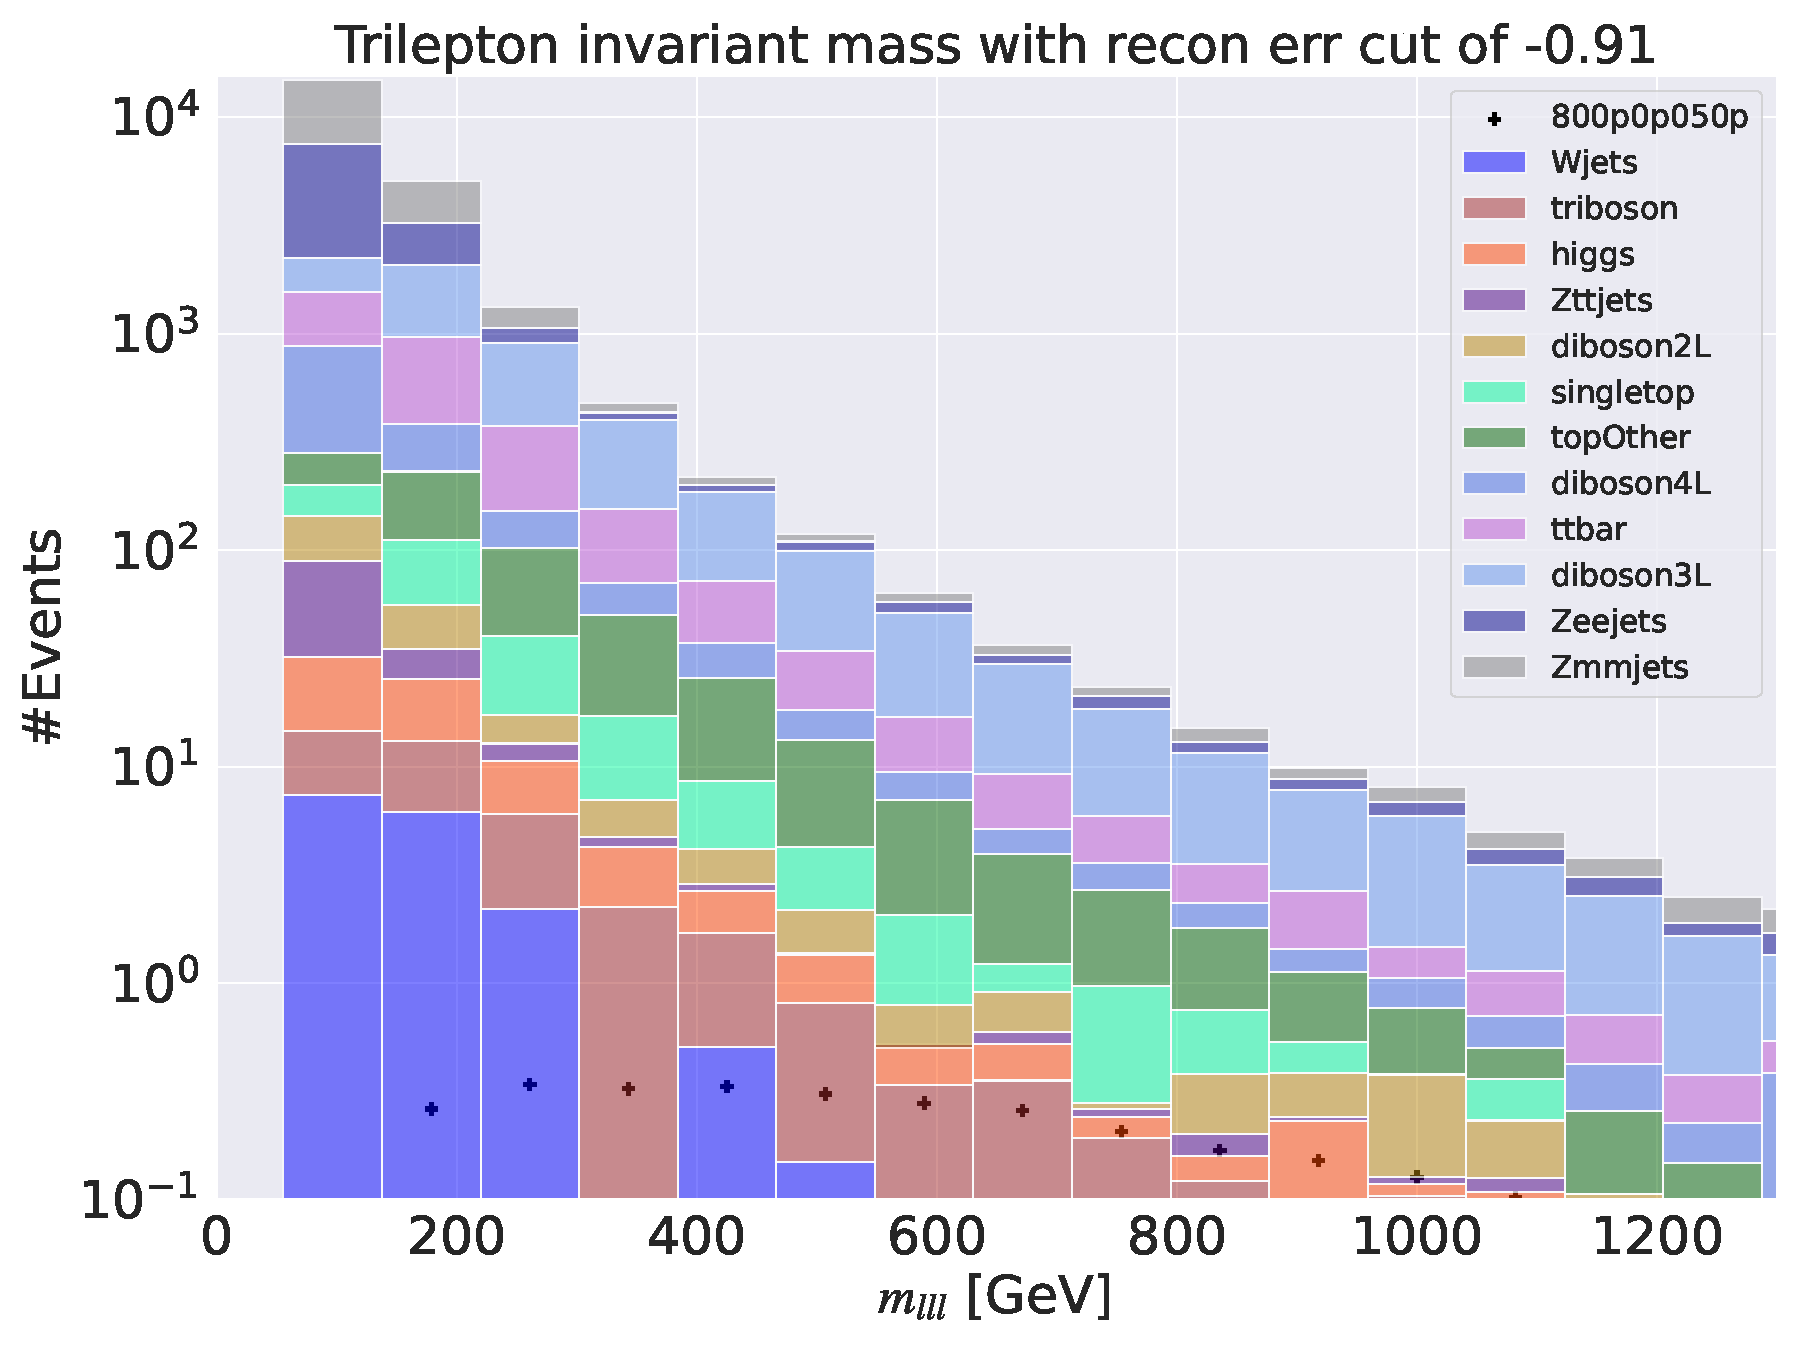
\includegraphics[width=\textwidth]{Figures/VAE_testing/small/3lep/b_data_recon_big_rm3_feats_sig_800p0p050p_mlll_recon_errcut_-0.91.pdf}
        \caption{}
        \label{fig:VAE_3lep_small_mlll_800}
    \end{subfigure}
    \hfill   
    \begin{subfigure}{.49\textwidth}
        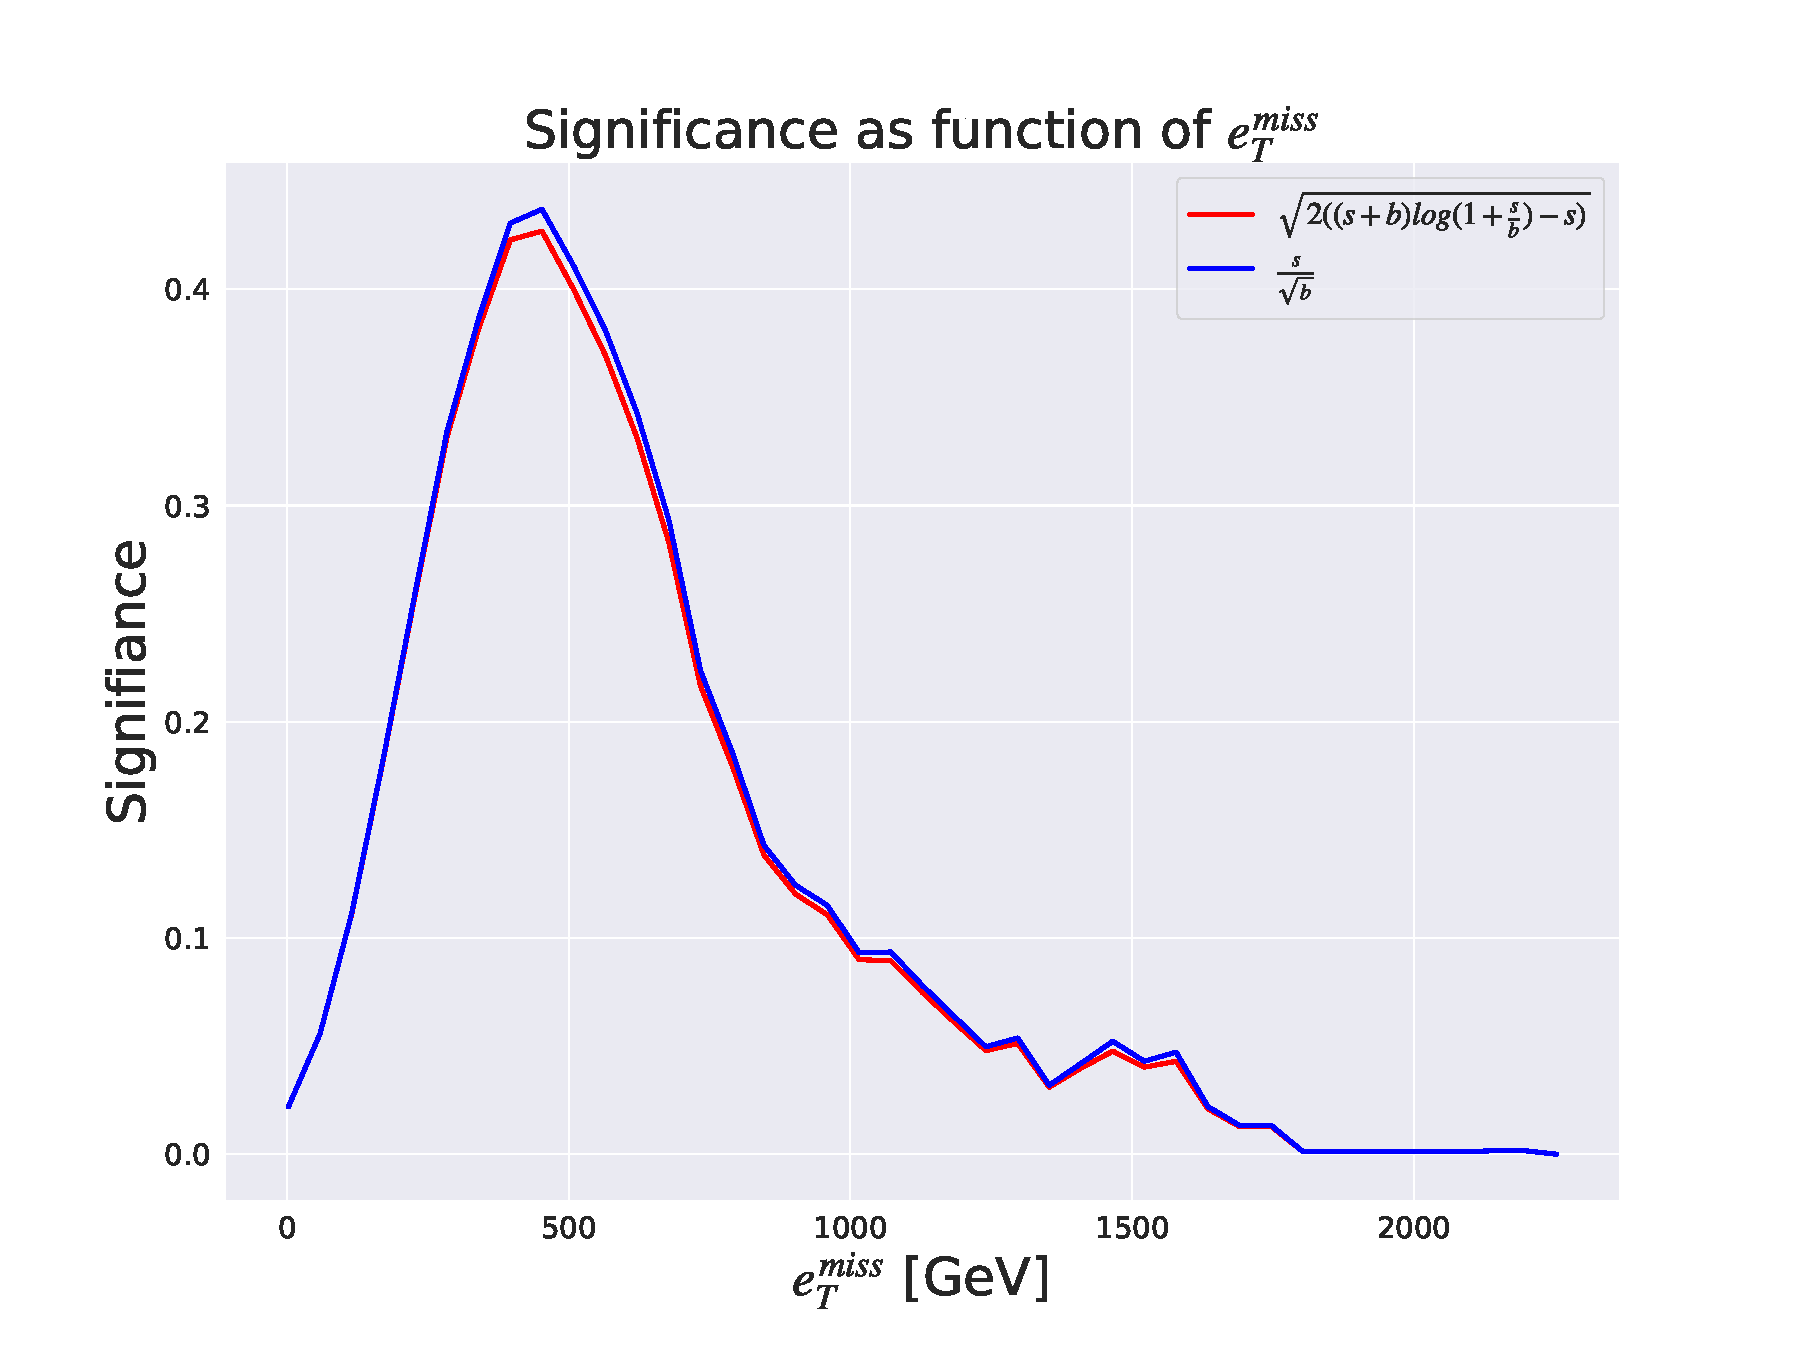
\includegraphics[width=\textwidth]{Figures/VAE_testing/small/3lep/significance_etmiss_800p0p050p_-0.9142561918890106.pdf}
        \caption{}
        \label{fig:VAE_3lep_small_signi_800}
    \end{subfigure}
    \hfill      
    \caption[3lep shallow network | $800p50$ | VAE]{Reconstruction error, $e_T^{miss}$ signal region, $m_{lll}$ signal region and significance as function of 
    $e_T^{miss}$ for the shallow variational autoencoder using the SUSY $800p50$.
    Figure \ref{fig:VAE_3lep_small_800} shows the reconstruction error 
    distribution for the SM MC and the SUSY signal. Here the autoencoder produces a hill-like for background and 
    signal with little destinction. The peaks of the two distributions are not separated in reconstruction error. Figure \ref{fig:VAE_3lep_small_etmiss_800} 
    shows the $e_T^{miss}$ distribution for the SM MC and the SUSY signal in the signal region, defined as the region having a $log_{10}$ reconstruction error above -0.91. 
    Some background is removed, and the peaks of the SM MC and signal 
    distributions are separated. Figure \ref{fig:VAE_3lep_small_mlll_800} shows the $m_{lll}$ distribution for the SM MC and the SUSY signal. 
    The shape of the SM MC and the signal distributions are displaying almost the same shape. Figure \ref{fig:VAE_3lep_small_signi_800} shows the significance as 
    function of $e_T^{miss}$. The maximum significance is found when applying a cut of about > 480 GeV in the $e_T^{miss}$, with a significance of around $0.45$.}
    \label{fig:VAE_3lep_small_rec_sig_signi_800}
\end{figure}

The corresponding results for the variational autoencoders are shown in 
Figure \ref{fig:VAE_3lep_big_rec_sig_signi_450} - \ref{fig:VAE_3lep_small_rec_sig_signi_800} 
following the same outline as used in section \ref{sec:3lep_red}.
From figures \ref{fig:VAE_3lep_big_450}, \ref{fig:VAE_3lep_small_450},
\ref{fig:VAE_3lep_big_800} and \ref{fig:VAE_3lep_small_800} we observe that the variational 
autoencoder seems to struggle with differentiating between background and signal. 
There is however a slight difference in the shape of the distributions from the shallow and 
deep network shown for both of the SUSY signal samples. The shallow VAEs have typically a more narrow and slightly more 
left-skewed shape, whereas the deep network has a slightly more broad distribution shifted a 
bit to the right. The bulk of the events for all four histograms are between $10^{-2}$ and $10^{-0.5}$ 
reconstruction error, indicating that the autoencoder struggles to learn the internal RMM 
structures for the 3 lepton + $e_T^{miss}$ final state MC. \par 
In figures \ref{fig:VAE_3lep_big_etmiss_450}, \ref{fig:VAE_3lep_small_etmiss_450}, 
\ref{fig:VAE_3lep_big_etmiss_800} and  \ref{fig:VAE_3lep_small_etmiss_800} we have the 
reconstruction error cut imposed on the SM MC and the signal samples. Interestingly, one should 
note that although the total reconstruction error distributions are not well separated, the 
signal regions show a separation in the $e_T^{miss}$ distribution. Unlike in the regular autoencoder 
case, the variational autoencoder allows for almost two orders of magnitude more background 
events in the signal region. This is because of the signal region definition from section 
\ref{sec:strategy} where the median for all four cases with the variational autoencoder is exactly at the peak of the 
reconstruction error distribution for the background. Therefor we also get the peak of 
the signal distributions, which is why we see so much signal in the signal region in figures 
\ref{fig:VAE_3lep_big_etmiss_450}, \ref{fig:VAE_3lep_small_etmiss_450}, 
\ref{fig:VAE_3lep_big_etmiss_800} and \ref{fig:VAE_3lep_small_etmiss_800}. \par 
As expected the separation between SM MC and signal in the $m_{lll}$ distribution, shown in 
Figure \ref{fig:VAE_3lep_big_mlll_450} -  \ref{fig:VAE_3lep_small_mlll_800},
is less prominent compared with the $e_T^{miss}$ distribution. The performance of the deep and shallow VAE, 
based on the separation of SM MC and signal in the signal regions,  are very similar.\par 
In figures \ref{fig:VAE_3lep_big_signi_450}, \ref{fig:VAE_3lep_small_signi_450}, \ref{fig:VAE_3lep_big_signi_800} and  
\ref{fig:VAE_3lep_small_signi_800} we have the significance as a function of the $e_T^{miss}$.
Interestingly, for the SUSY $450p300$ case, we have that both the deep and shallow 
autoencoder manages to get a significance of around 4, which is much better than the 
regular autoencoder which got around 0.7. For the SUSY $800p50$ signal the difference between the significance 
from the AE and VAE was small. A cut at etmiss > 400 GeV provided the best significance of around 4.5 for the $450p300$ 
signal point using the signal region defined by a cut in the reconstruction error of $10^{-1.1}$ $(10^{-1.06})$ 
using a deep (shallow) VAE.
